\documentclass[a4paper,11pt,openany]{ltjsbook}
\usepackage{luatexja}
\usepackage{luatexja-fontspec}
\usepackage{amsmath,amssymb,amsfonts,amsthm}
\usepackage{graphicx}
\usepackage{geometry}
\geometry{top=24mm,bottom=24mm,left=24mm,right=24mm,footskip=10mm}
\usepackage{tcolorbox}
\tcbuselibrary{skins,breakable}
\usepackage{hyperref}
\usepackage{enumitem}
\usepackage{booktabs}
\usepackage{fancyhdr}

\definecolor{geomblue}{RGB}{20, 50, 90}
\definecolor{goldaccent}{RGB}{180, 130, 20}
\definecolor{softblue}{RGB}{245, 248, 252}

\hypersetup{
    colorlinks=true,
    linkcolor=geomblue,
    citecolor=goldaccent,
    urlcolor=geomblue
}

\pagestyle{fancy}
\fancyhf{}
\fancyhead[LE,RO]{\thepage}
\fancyhead[LO]{\nouppercase{\rightmark}}
\fancyhead[RE]{\nouppercase{\leftmark}}
\renewcommand{\headrulewidth}{0.4pt}

\title{\Huge\textbf{非ユークリッド幾何学}\\[4mm]
\huge\textbf{公理から拡がる双曲・楕円幾何学の体系}\\[6mm]
\Large\textbf{全訳・数理解説版}\\[5mm]
\large ヘンリー・パーカー・マニング 著（Henry Parker Manning, 1901）\\[2mm]
\normalsize Project Gutenberg eBook \#13702: \textit{Non-Euclidean Geometry}}

\author{\textbf{数理文献翻訳プロジェクト} 編訳}
\date{2026年11月 決定版}

\begin{document}

\maketitle

\frontmatter
\tableofcontents

\chapter{序文}

非ユークリッド幾何学は、いまや数学の重要な一分野として認められている。幾何学を教える者はこの主題について何らかの知識をもつべきであり、数学に関心のある者はみな、この幾何学が示す新奇な結果や見方のなかに、多くの刺激と楽しみを見いだすだろう。

本書は、非ユークリッド幾何学を、簡明かつ直接的に述べようとする試みであり、数学の予備知識をほとんど前提としない。最初の三つの章は、平面幾何・立体幾何・三角法の知識だけを前提としており、本書全体は、大学で通常課される数学の課程を修めた者であれば読み通すことができる。

ここに公にするものに、独創性を主張すべき点は特にない。命題はいずれも古くから、さまざまな方法で確立されてきた。証明のなかには新しいものもあるかもしれないが、この主題の著者たちがすでに与えたもののなかには、これ以上改良しようのないものもある。それらは、主としてテキサス大学のジョージ・ブルース・ハルステッド教授の翻訳を通じて私のもとに伝わった。

ロードアイランド州ヴァレーフォールズのアーノルド・B・チェイス理学博士には、とりわけ恩義を受けている。この主題を共に学び、論じた友人である。

\bigskip
\begin{flushright}
ヘンリー・P・マニング

\small プロビデンス、1901年1月
\end{flushright}

\chapter{序論}

幾何学の公理は、かつては思考の法則とみなされ、聡明な精神であれば否定することも吟味することもできないものと考えられていた。われわれが慣れ親しんできた公理が経験とよく一致することが見いだされたばかりでなく、それらのどれかが成り立たないという仮定のもとでは推論することすらできない、と信じられていた。しかし今では、ユークリッドの公理と全体として、あるいは一部分において矛盾する公理の組を採用しても、ユークリッドの幾何学と同じように無矛盾な幾何学を築き上げることができる、ということが示されている。

ここでは、最も重要な二つの非ユークリッド幾何学を示す。\footnote{「歴史的注」（本書末）を見よ。}これらでは、平行線に関するもの以外の公理と定義は、ユークリッドのとおりに採る。平行線についての公理を除くと、三つの仮説に至る。その一つはユークリッドの幾何学を確立し、他の二つはそれぞれ、興味深くかつ有用な一連の命題を与える。実際、宇宙のうち限られた部分しか調べることができない以上、ユークリッドの体系が、これから述べる二つの非ユークリッド幾何学のいずれよりも真であることを証明することはできない。

配列は次のようにする。まず三つの幾何学に共通する命題を証明し、つぎにユークリッドと異なる二つの幾何学のそれぞれについて、一連の命題と三角法の公式を導き、最後に解析的方法によって、それらの最も顕著な性質のいくつかを導く。

幾何学の基礎を直接に調べることも、この研究で意識的にせよ無意識的にせよなされた仮定をすべて指摘することも、ここでは意図しない。これらの幾何学に共通なものには手をつけずにおくことで、それらの相違点だけに注意を集中することができる。抽象的な理論だけによるよりも、具体的な叙述によるほうが、幾何学の本性についてより多くを学べるかもしれない。

そこで、幾何学の用語の大部分は、教科書に与えられている定義をくり返すことなく用い、これらの用語で定義される図形が存在するものと仮定する。特に、次を仮定する。
\smallskip

\begin{enumerate}
\item[I.] \emph{任意の二点によって定まる直線が存在すること、および二点間の最短の道は直線であること。}

\item[II.] \emph{一直線上にない任意の三点によって定まる平面が存在すること、および平面上の任意の二点を結ぶ直線は完全にその平面に含まれること。}

\item[III.] \emph{幾何学的図形は、形も大きさも変えずに動かすことができること。}

\item[IV.] \emph{点が直線上をある位置から別の位置へ動くとき、その間のすべての点を通ること、また、たとえば角や線分の長さのような幾何学的な量がある値から別の値まで変化するとき、その間のすべての値をとること。}
\end{enumerate}

いくつかの命題では、細部を普通の教科書から補えるものについて、証明を省くか、証明の方法を示すだけにとどめる。


\mainmatter

\chapter{汎幾何学}

\section{重ね合わせの原理のみに依存する命題}

\begin{description}
\item[1.~定理.] \emph{一つの直線が別の直線と出会うとき、できる隣り合う角の和は二直角に等しい。}

\item[2.~定理.] \emph{二直線が交わるとき、対頂角は等しい。}

\item[3.~定理.] \emph{二つの三角形において、一方の一辺とその両端の角、または二辺とその間の角が、他方の対応する部分にそれぞれ等しければ、二つの三角形は等しい。}

\item[4.~定理.] \emph{二等辺三角形では、等しい辺に対する角は等しい。}

頂角を二等分し、(3) を用いる。

\item[5.~定理.] \emph{三角形の各辺の中点に立てた垂線のうち二本が交わるならば、三本は一点で交わり、この点は三角形の三つの頂点を通る円の中心である。}

\begin{figure}[h]
\centering
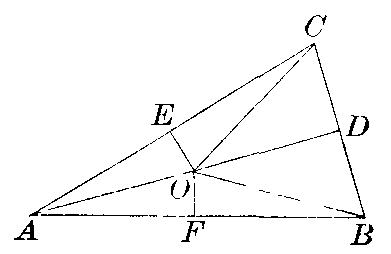
\includegraphics[width=40mm]{fig01.png}
\end{figure}

\textbf{証明.} $EO$ と $FO$ が $O$ で交わるとする。三角形 $AFO$ と $BFO$ は (3) により等しい。また $AEO$ と $CEO$ も等しい。したがって $CO$ と $BO$ は、ともに $AO$ に等しいから、等しい。ゆえに三角形 $BCO$ は二等辺三角形であり、角 $BOC$ を二等分するように引いた $OD$ は、$BC$ に対してその中点で垂直になる。

\item[6.~定理.] \emph{円において、中心での角を二等分する半径は、その角に対する弦に垂直であり、この弦を二等分する。}

\item[7.~定理.] \emph{円の中心における角は、切り取られる弧に比例し、弧によって測ることができる。}

\item[8.~定理.] \emph{直線外の任意の点から、その直線へ垂線を引くことができる。}

\begin{figure}[h]
\centering
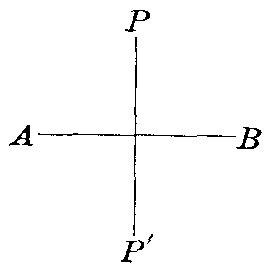
\includegraphics[width=20mm]{fig02.png}
\end{figure}

\textbf{証明.} 平面を $AB$ のまわりに回転させて自分自身に重ね合わせたとき、点 $P$ が移る位置を $P'$ とする。そのとき、直線 $PP'$ は $AB$ に垂直である。

\item[9.~定理.] \emph{直線に立てた垂線上の一点から斜線を引き、垂線の足から等しい距離のところを切り取るならば、それらの斜線は等しく、直線となす角も垂線となす角も等しい。}

\begin{figure}[h]
\centering
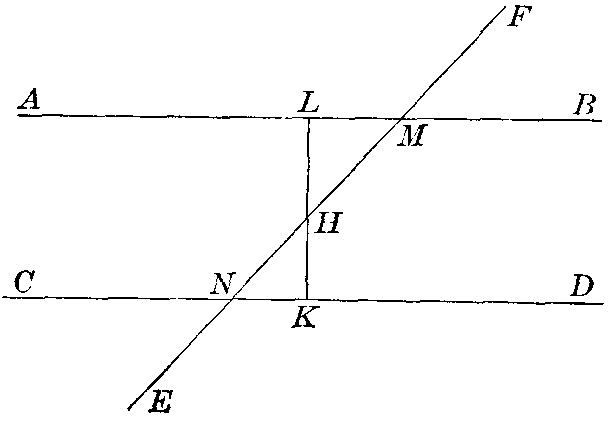
\includegraphics[width=50mm]{fig03.png}
\end{figure}

\item[10.~定理.] \emph{二直線が第三の直線と同じ角で交わる、すなわち対応する角が等しいならば、その二直線の両方に垂直な直線を引くことができる。}

\textbf{証明.} 角 $FMB$ と $MND$ が等しいとし、$MN$ の中点 $H$ を通って $CD$ に垂直に $LK$ を引く。このとき $LK$ は $AB$ にも垂直である。なぜなら、二つの三角形 $LMH$ と $KNH$ が (3) により等しいからである。

\item[11.~定理.] \emph{平面上で、与えられた直線に垂直に立てた等しい二本の線分があるとき、それらの端点を結ぶ線は二本の線分と等しい角をなし、両者の中間に立てた第三の垂線によって、直角に二等分される。}

\begin{figure}[h]
\centering
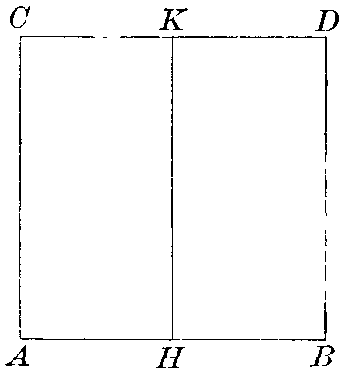
\includegraphics[width=40mm]{fig04.png}
\end{figure}

\textbf{$AC$ と $BD$} が $AB$ に垂直で、$AC$ と $BD$ が等しいとする。$C$ と $D$ を結ぶ線が $C$ と $D$ でなす角は等しく、$AB$ の中点に立てた垂線 $HK$ は、$CD$ に対してその中点で垂直である。

重ね合わせにより証明される。

\item[12.~定理.] \emph{前の命題のように二本の垂線と、その中間に立てた第三の垂線が与えられているとき、この第三の垂線に直角に交わる任意の直線は、最初の二本と交わるならば、それらの上に等しい長さを切り取り、等しい角をなす。}

重ね合わせにより証明される。

\begin{figure}[h]
\centering
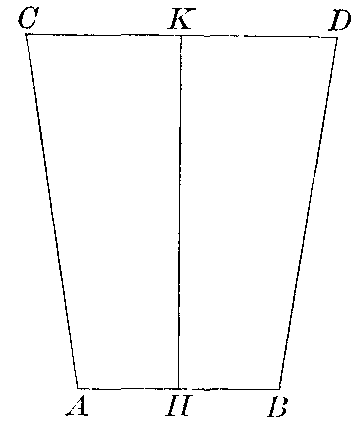
\includegraphics[width=40mm]{fig05.png}
\end{figure}

\textbf{系.} \emph{前の二つの命題は、$A$ と $B$ での角が等しい鋭角、または等しい鈍角であって、$HK$ が $AB$ の中点で $AB$ に垂直である場合にも成り立つ。$AC = BD$ ならば、$C$ と $D$ での角は等しく、$HK$ は $CD$ に対してその中点で垂直である。または、$CD$ が $HK$ に任意の点 $K$ で垂直であり、$AC$ と $BD$ と交わるならば、それはこの二直線上に等しい距離を切り取り、等しい角をなす。}
\end{description}

\section{限定された図形について成り立つ命題}

つぎの命題は、少なくとも、線の長さがある一定の長さを超えない図形について成り立つ。すなわち、例外があるとしても、それは線のどこかの長さのために、定理あるいは証明のある段階を適用できないような場合にあたる。便宜上、この意味で\emph{限定された}という語を用い、ある定理が限定された図形について、あるいは平面の限定された部分において成り立つ、と言うことにする。

\begin{figure}[h]
\centering
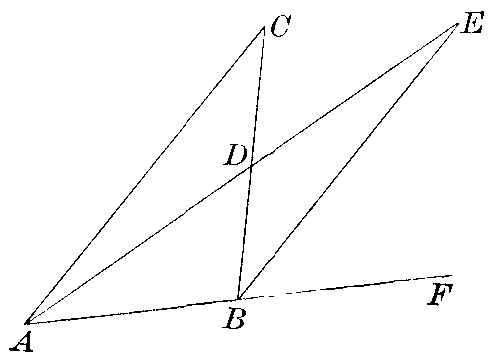
\includegraphics[width=40mm]{fig06.png}
\end{figure}

\begin{description}
\item[1.~定理.] \emph{三角形の外角は、それに隣り合わない内角のどちらよりも大きい}（ユークリッド、I, 16）。

\textbf{証明.} $A$ から対辺の中点まで $AD$ を引き、それを延長して $DE = AD$ となるように $E$ をとる。二つの三角形 $ADC$ と $EBD$ は等しく、角 $FBD$ は角 $EBD$ より大きいから、$C$ より大きい。

\textbf{系.} \emph{三角形の少なくとも二つの角は鋭角である。}

\item[2.~定理.] \emph{三角形の二つの角が等しければ、それに対する辺は等しく、その三角形は二等辺三角形である。}

\begin{figure}[h]
\centering
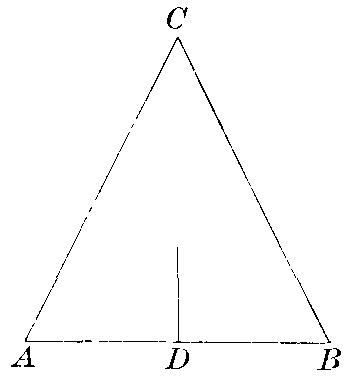
\includegraphics[width=40mm]{fig07.png}
\end{figure}

\textbf{証明.} 底辺の中点に立てた垂線は、三角形を、互いに重ね合わせることができて等しい二つの図形に分ける。したがってこの垂線は頂点を通り、等しい角に対する二辺は等しい。

\item[3.~定理.] \emph{角が等しくない三角形では、大きいほうの角に対する辺は、小さいほうの角に対する辺より大きい。逆に、三角形の辺が等しくなければ、対する角も等しくなく、大きい角は大きい辺に対する。}

\item[4.~定理.] \emph{二つの三角形において、一方の二辺が他方の二辺にそれぞれ等しく、しかも第一の三角形の挟む角が第二の三角形の挟む角より大きいならば、第一の三角形の第三辺は第二の三角形の第三辺より大きい。逆に、二つの三角形において、一方の二辺が他方の二辺にそれぞれ等しく、しかも第一の三角形の第三辺が第二の三角形の第三辺より大きいならば、第一の三角形の第三辺に対する角は、第二の三角形の第三辺に対する角より大きい。}

\item[5.~定理.] \emph{任意の点から直線の両端へ引いた二線の和は、同様に引いてそれらに囲まれた二線の和より大きい。}

\item[6.~定理.] \emph{一点を通って直線へ引ける垂線は、ただ一本である。}

\begin{figure}[h]
\centering
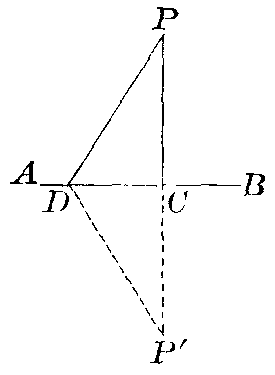
\includegraphics[width=30mm]{fig08.png}
\end{figure}

\textbf{証明.} 平面を $AB$ のまわりに回転させて自分自身に重ね合わせたとき、点 $P$ が移る位置を $P'$ とする。$P$ から $AB$ へ二本の垂線 $PC$ と $PD$ が引けるとすると、$CP'$ と $DP'$ はこれらの線の延長となり、$P$ と $P'$ を結ぶ異なる二本の直線ができることになるが、それは不可能である。

\textbf{系.} \emph{二つの直角三角形は、一方の斜辺と一つの鋭角が、他方の斜辺と一つの鋭角にそれぞれ等しいとき、等しい。}

\item[7.~定理.] \emph{垂線は、点から直線へ引くことのできる線のうちで最も短い。}

\textbf{系.} \emph{直角三角形では、斜辺は、直角をはさむ二辺のどちらよりも大きい。}

\item[8.~定理.] \emph{直線に立てた垂線上の一点から斜線を引き、垂線の足から等しくない距離のところを切り取るならば、それらの斜線は等しくなく、遠いほうが大きい。逆に、垂線上の一点から引いた二本の斜線が等しくなければ、大きいほうが垂線の足からより大きい距離を切り取る。}

\item[9.~定理.] \emph{線分の中点に垂線を立てたとき、その垂線上にない任意の点は、垂線に関して同じ側にある線分の端点により近い。}

\textbf{系.} \emph{線分の両端から等距離にある二点は、その線分にその中点で垂直な直線を決定する。}

\item[10.~定理.] \emph{二つの三角形は、一方の三辺が他方の三辺にそれぞれ等しいとき、等しい。}

\item[11.~定理.] \emph{平面上で、第三の直線に垂直に立てた二本の線が等しくなければ、それらの端点を結ぶ線が二本の線となす角も等しくなく、短い垂線とのなす角のほうが大きい。}

\begin{figure}[h]
\centering
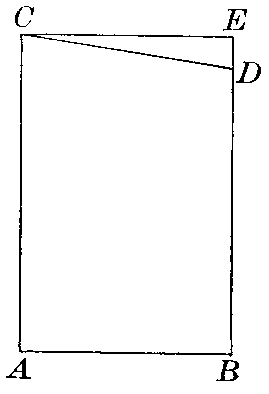
\includegraphics[width=25mm]{fig09.png}
\end{figure}

\textbf{証明.} $AC > BD$ とする。$BD$ を延長して $BE = AC$ とする。すると $BEC = ACE$ である。しかし (1) により $BDC > BEC$ であり、$ACD$ は $ACE$ の一部である。したがって、なおさら $BDC > ACD$ である。

\item[12.~定理.] \emph{$C$ と $D$ での二つの角が等しければ、垂線は等しく、角が等しくなければ、垂線も等しくなく、長いほうの垂線は小さいほうの角をなす。}

\item[13.~定理.] \emph{二直線が第三の直線に垂直であるとき、一方の直線上の点で第三の直線から等距離にあるものは、他方の直線からも等距離にある。}

\begin{figure}[h]
\centering
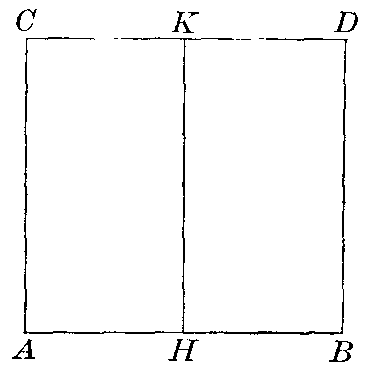
\includegraphics[width=30mm]{fig10.png}
\end{figure}

\textbf{証明.} $AB$ と $CD$ が $HK$ に垂直であるとし、$CD$ 上に $K$ から等距離にある任意の二点 $C$ と $D$ をとる。すると $C$ と $D$ は $AB$ から等距離にある。なぜなら、重ね合わせにより $D$ を $C$ に重ねることができ、そのとき (6) により $DB$ は $CA$ に重なるからである。
\end{description}

\medskip 立体幾何学のつぎの命題は、直接に前の諸命題に依存し、少なくとも空間の任意の限定された部分で成り立つ。

\begin{description}
\item[14.~定理.] \emph{一直線が、交わる二直線にその交点で垂直ならば、それは、その交点を通る二直線の平面上のすべての直線に垂直である。}

\item[15.~定理.] \emph{二つの平面が垂直ならば、一方の平面内でそれらの交線に垂直に引いた直線は、他方の平面に垂直である。また、一方の平面の任意の点を通って他方の平面に垂直に引いた直線は、完全に前者の平面内にある。}

\item[16.~定理.] \emph{直線が平面に垂直ならば、その直線を通る任意の平面は、その平面に垂直である。}

\item[17.~定理.] \emph{平面が、交わる二つの平面のそれぞれに垂直ならば、その平面はそれらの交線に垂直である。}
\end{description}

\section{三つの仮説}

二本の等しい垂線の端点での角は、少なくとも限定された図形については、直角か、鋭角か、鈍角のいずれかである。この三つの場合を、それぞれ\emph{直角の仮説}、\emph{鋭角の仮説}、\emph{鈍角の仮説}と呼んで区別する。

\begin{description}
\item[1.~定理.] \emph{二本の等しい垂線の端点を結ぶ線は、少なくとも平面の任意の限定された部分では、三つの仮説に応じて、それぞれ垂線の足を結ぶ線に等しいか、より大きいか、より小さい。}

\begin{figure}[h]
\centering
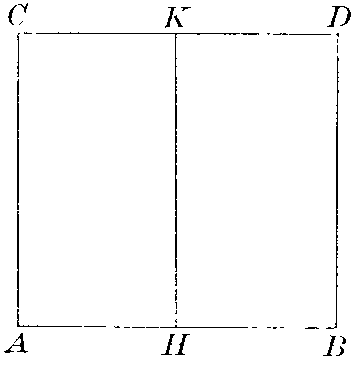
\includegraphics[width=35mm]{fig11.png}
\end{figure}

\textbf{証明.} $AC$ と $BD$ を二本の等しい垂線とし、$HK$ を $AB$ の中点に立てた第三の垂線とする。このとき $HA$ と $KC$ は $HK$ に垂直であり、$C$ での角が $A$ での角に等しいか、より小さいか、より大きいかに応じて、$KC$ は $HA$ に等しいか、より大きいか、より小さい（II, 12）。したがって、$KC$ の二倍である $CD$ は、三つの仮説に応じて、それぞれ $AB$ に等しいか、より大きいか、より小さい。

\textbf{逆に、}$CD$ が $AB$ に等しいか、より大きいか、より小さいと与えられるならば、この図形について、それぞれ第一、第二、第三の仮説が成り立つ。

\textbf{系.} \emph{四角形が三つの直角をもつとき、第四の角に隣り合う辺は、第四の角が直角か、鋭角か、鈍角かに応じて、それぞれの対辺に等しいか、より大きいか、より小さい。}

\item[2.~定理.] \emph{直角の仮説が、平面の任意の限定された部分における一つの場合に成り立つならば、それはあらゆる場合に、平面全体で成り立つ。}

\begin{figure}[h]
\centering
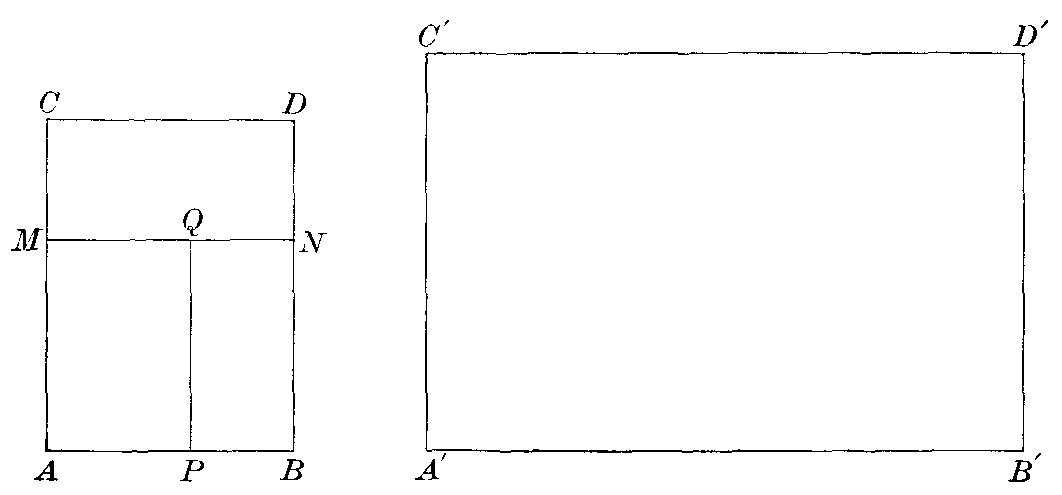
\includegraphics[width=75mm]{fig12.png}
\end{figure}

\textbf{証明.} ここでは長方形、すなわち四つの角がすべて直角の四角形がある。前の命題の系により、その対辺は等しい。等しい長方形は、辺が与えられた長方形の対応する辺の任意の倍数となるような長方形をつくるように、並べて置くことができる。

さて、$A'B'$ を任意の線分とし、$A'C'$ と $B'D'$ をその両端で $A'B'$ に垂直な等しい二線とする。$A'C'$ を、必要ならばいくつかの等しい部分に分けて、その一つが $AC$ より小さくなるようにし、$AC$ と $BD$ の上に、そのうちの一つに等しい $AM$ と $BN$ をとり、$MN$ を引く。$ABNM$ は長方形である。そうでなければ、$MN$ は $AB$ と $CD$ より大きいか小さいかであり、$M$ と $N$ での角はすべて鋭角か、すべて鈍角になるが、それらの和はちょうど四直角であるから、これは不可能である。つぎに、$A'B'$ を十分な個数の等しい部分に分け、その一つを $AB$ と $MN$ 上にとり、長方形 $APQM$ をつくる。これに等しい長方形を並べて、図形 $A'B'D'C'$ をちょうど覆うことができるから、この図形自身も長方形でなければならない。

\item[3.~定理.] \emph{鋭角の仮説または鈍角の仮説が、平面の限定された部分内の一つの場合に成り立つならば、同じ仮説が、平面のそのような任意の部分内のあらゆる場合に成り立つ。}

\begin{figure}[h]
\centering
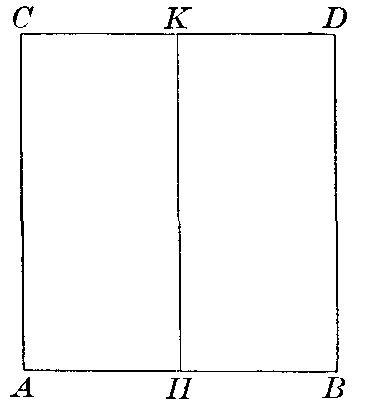
\includegraphics[width=35mm]{fig13.png}
\end{figure}

\textbf{証明.} $CD$ を $AC$ と $BD$ に沿って動かし、この二線上に常に等しい距離を切り取るようにする。あるいはまた、$AC$ と $BD$ を線 $AB$ に沿って $HK$ のほうへ、または $HK$ から遠ざかるように動かし、つねに $AB$ に垂直であって、その足が $H$ から常に等距離にあるようにする。$C$ と $D$ での角は連続的に変化するから、鋭角あるいは鈍角のままでいるか、あるいはどこかで直角になるかのいずれかでなければならない。直角になるとすれば、直角の仮説が成り立つことになり、仮定した一つの場合においてすら、鋭角の仮説も鈍角の仮説も成り立ち得ない。

$C$ と $D$ での角は、平面の限定された部分では、零にも $180^\circ$ にもなり得ない。なぜなら、そうなれば三つの線 $AC$、$CD$、$BD$ が同一の直線になってしまうからである。

\item[4.~定理.] \emph{三角形の内角の和は、少なくとも平面の任意の限定された部分では、三つの仮説に応じて、それぞれ二直角に等しいか、より小さいか、より大きい。}

\begin{figure}[h]
\centering
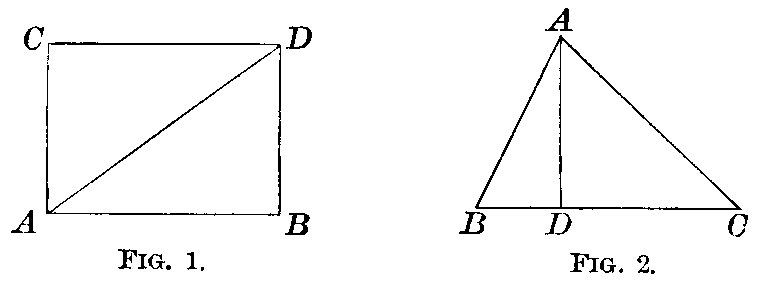
\includegraphics[width=80mm]{fig14.png}
\end{figure}

\textbf{証明.} $B$ に直角をもつ任意の三角形 $ABD$（図1）が与えられたとして、$AB$ に垂直に、$BD$ に等しい $AC$ を引く。三角形 $ADC$ と $DAB$ において、$AC=BD$ で $AD$ は共通であるが、$DC$ は三つの仮説に応じて、それぞれ $AB$ に等しいか、より大きいか、より小さい。したがって、$DAC$ は三つの仮説に応じて、それぞれ $ADB$ に等しいか、より大きいか、より小さい（II, 4）。この二つの角のそれぞれに $BAD$ を加えると、$ADB + BAD$ は直角 $BAC$ に等しいか、それより小さいか、それより大きいことになる。

さて、限定された任意の三角形の少なくとも二つの角は鋭角である。したがって、第三の角の頂点から対辺へ下ろした垂線は、その辺と三角形の内部で出会い、三角形を二つの直角三角形に分ける。ゆえに、限定された任意の三角形において、角の和は三つの仮説に応じて、それぞれ二直角に等しいか、より小さいか、より大きい。

三角形の角の和が二直角を超える量を、その\emph{過剰}と呼ぶ。$n$ 辺の多角形の過剰とは、その角の和が二直角の $n-2$ 倍を超える量である。

辺上の任意個の点を付加的な頂点と数えても、過剰は変わらない。このとき角の和には、そのような点ごとに二直角が加わるからである。

\item[5.~定理.] \emph{多角形の過剰は、それを分割してできる三角形の任意の系の過剰の和に等しい。}

\begin{figure}[h]
\centering
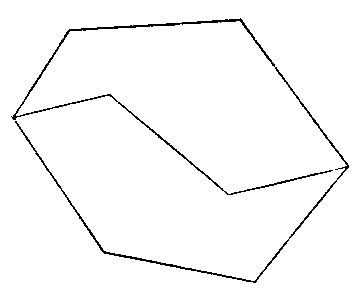
\includegraphics[width=30mm]{fig15.png}
\end{figure}

\textbf{証明.} 多角形を直線または折れ線で二つの多角形に分けるとき、その線が境界と出会う二点は頂点であるとしてよい。分割する線が $p$ 個の点で折れる折れ線であるならば、二つの多角形の辺は、もとの多角形の辺と、分割線が $p$ 個の点で分けられてできる $p+1$ 個の部分（それぞれ二度ずつ数える）とからなる。

もとの多角形の角の和を $S$、辺の数を $n$ とする。それが分けられてできた二つの多角形について、$S'$ と $n'$、$S''$ と $n''$ は同じ意味をもつとする。直角を $R$ と書くと、
\begin{align*}
S' + S'' &= S + 4pR, \\
\intertext{および}
n' + n'' &= n + 2(p+1). \\
\intertext{したがって、}
S' - 2(n'-2)R + S'' - 2(n''-2)R &= S + 4pR - 2(n+2p-2)R \\
&= S-2(n-2)R.
\end{align*}

多角形を分割してできる三角形の任意の系は、以上の過程を十分な回数くり返すことによって得られる。多角形の過剰は、つねに、それを分割してできる部分の過剰の和に等しい。

過剰の概念を拡張して、完全に直線で囲まれた平面の異なる部分の、任意の組み合わせに適用することもできる。

多角形の角の和を考える代わりに、外角の和をとってもよい。この和が四直角に足りない量は、多角形の過剰に等しい。これを外角の\emph{不足}ということができる。

\begin{figure}[h]
\centering
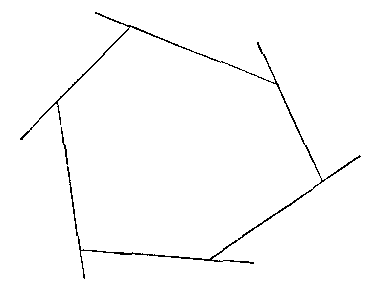
\includegraphics[width=30mm]{fig16.png}
\end{figure}

外角の和は、図形のまわりをちょうど一周するとき、各頂点で一つの辺から次の辺へ向きを変える、その回転量である。二つ以上の多角形の組み合わせを考えるときは、考える領域がつねに一方の側、たとえば左側にあるように、境界全体をたどらなければならない。

\item[6.~定理.] \emph{多角形の過剰は、つねに零であるか、つねに負であるか、つねに正である。}

\textbf{証明.} この定理が、限定された三角形について成り立つことはわかっている。しかし、有限な多角形は、有限個のそのような三角形に分割できるから、前の定理により、多角形の過剰はそれらの三角形の過剰の和に等しい。

過剰が負であるときは、それを不足と呼ぶか、外角の過剰と言うことができる。

\textbf{系.} \emph{多角形の過剰は、直線によってそれから切り取られる任意の部分の過剰より、数値として大きい。ただし第一の仮説では零である。}
\end{description}

\medskip つぎの定理は、第二および第三の仮説に適用される。


\begin{description}
\item[7.~定理.] \emph{三角形の辺を小さくしてゆくことにより、あるいは、他の二辺がある一定の長さより小さいままで一辺だけを小さくすることによってさえ、その面積を限りなく小さくでき、その角の和は二直角に限りなく近づく。}

\begin{figure}[h]
\centering
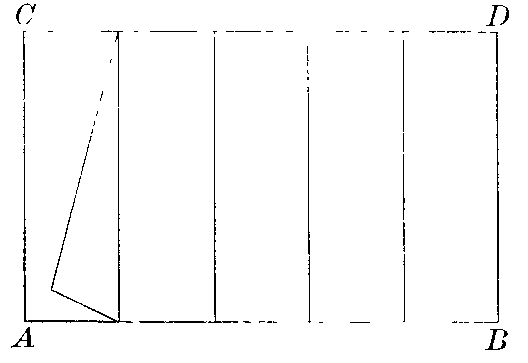
\includegraphics[width=50mm]{fig17.png}
\end{figure}

\textbf{証明.} $ABDC$ を、$A$、$B$、$C$ に三つの直角をもつ四角形とする。$AB$ に沿って動く垂線は、つねに増加するか、つねに減少する。なぜなら、もしある範囲では増加し、ある範囲では減少するとすれば、垂線が同じ長さとなる位置が異なる二つあることになり、その中間にある垂線は $CD$ にも垂直になって、長方形ができてしまうからである。

$AB$ を $n$ 個の等しい部分に分け、分点を通って垂線を引く。四角形は $n$ 個のより小さい四角形に分けられ、これらは一辺とその両端の二つの直角がすべて同じであるから、互いに重ね合わせることができる。垂線が最も短いほうの端から始めると、各四角形は、次の四角形の内部に完全に収まるように置くことができる。したがって、最初の四角形の面積は、もとの四角形の面積の $\frac{1}{n}$ より小さく、その不足あるいは過剰も、全体の不足あるいは過剰の $\frac{1}{n}$ より小さい。さて、すべての辺が $AC$ または $BD$ より小さく、かつ一辺が $AB$ の小区間の一つより小さいような任意の三角形は、この最小の四角形の内部に完全に収めることができる。そのような三角形は、その面積と、不足あるいは過剰とが、もとの四角形の面積と、不足あるいは過剰との $\frac{1}{n}$ より小さい。

こうして、三角形は、少なくとも一辺を十分に小さくとれば、他の二辺が限りなく大きくなければ、その面積と不足あるいは過剰を、どれほど小さく指定された面積と不足あるいは過剰よりも小さくできる。

\item[8.~定理.] \emph{不足あるいは過剰が同じ二つの三角形は、面積が等しい。}

\begin{figure}[h]
\centering
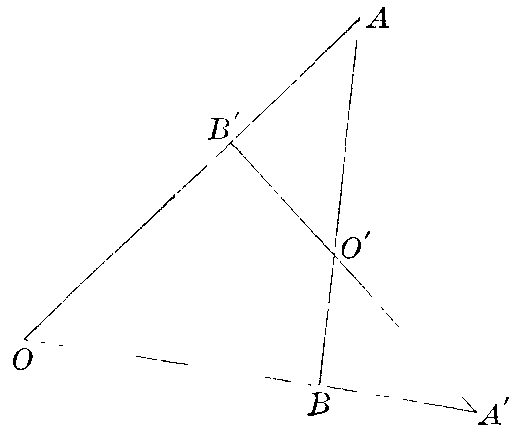
\includegraphics[width=40mm]{fig18.png}
\end{figure}

\textbf{証明.} $AOB$ と $A'OB'$ が、不足あるいは過剰が同じで、一方の一つの角が他方の一つの角に等しいとする。等しい角が重なるように二つを並べて置くと、二つの三角形は完全に重なって等しくなるか、あるいは二つに共通な四角形ができ、そのほかに、両方に共通な一つの角をもち、不足あるいは過剰が同じである二つのより小さな三角形が残る。これらを並べて置くと、ふたたび両方に共通な四角形と、両方に共通な一つの角をもち、不足あるいは過剰が同じである第三の三角形の組が得られる。この過程は、重なり合う三角形の組に出会わないかぎり、限りなく続けることができる。なぜなら、二つの三角形の不足あるいは過剰が同じであるから、組の一方の三角形が他方に完全に含まれることは、どの段階でもないからである。

最初の二つの三角形の、等しい角に対する辺の和を $so$、隣り合う辺の和を $sa$ とし、二つの三角形を並べて置いたときに両者に共通する、二度数えられる隣り合う辺の部分を $s'a$ とする。第二の三角形の組に $o'$ と $a'$、第三の組に $o''$ と $a'$、などを用いると、
\begin{gather*}
\begin{aligned}
sa   &= s'a + so',                 & so   &= sa',  \\
sa'  &= s'a' + so'',               & so'  &= sa'', \\
sa'' &= s'a'' + so'''\text{, etc.} & so'' &= sa''' \text{, etc.}
\end{aligned}\\
\begin{aligned}
\therefore sa  &= s'a  + s'a''  + s'a^{IV} + \ldots, \\
           sa' &= s'a' + s'a''' + s'a^{V}  + \ldots.
\end{aligned}
\end{gather*}

したがって、$s'a$、$s'a'$、$s'a''$、$\cdots$ は限りなく小さくなる。これらの各々は、三角形の組の一方から二度数えた一辺と、他方から二度数えた一辺とからなる。したがって、過程を十分遠くまで進めれば、残る三角形は、少なくとも一辺を望むだけ小さくでき、しかもすべての辺は小さくなって、たとえばもとの三角形の最長の辺より小さくなる。ゆえに、残る三角形の面積は限りなく小さくなるが、各組の三角形の面積の差は同じままなのだから、この差は零でなければならない。各組の三角形、とくに最初の二つの三角形は、面積が等しい。

\begin{figure}[ht]
\centering
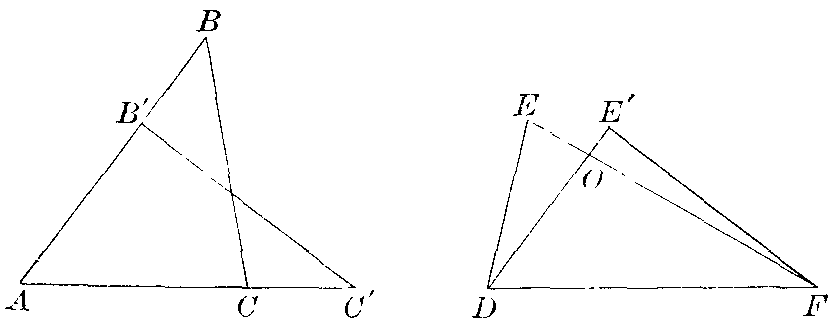
\includegraphics[width=70mm]{fig19.png}
\end{figure}

$ABC$ と $DEF$ の不足あるいは過剰が同じで、$AC<DF$ とする。$AC$ を $C'$ まで延長して $AC'$ = $DF$ とする。すると $AB$ 上の $A$ と $B$ の間に、$AB'C'$ が $ABC$ と同じ不足あるいは過剰と同じ面積をもつような点 $B'$ がある。$AB'C'$ を、$AC'$ が $DF$ に重なるように $DEF$ の上に置き、それが占める位置を $DE'F$ とする。二つの三角形が重ならなければ、共通の辺 $DF$ に対する各々の頂点は他方の外側にある。二つの三角形は共通に、たとえば三角形 $DOF$ をもち、そのほかに、二つの三角形のうちから、両方に同じ一つの角をもち、不足あるいは過剰が同じである二つのより小さな三角形が残る。この二つの三角形は、したがってもとの三角形も、面積が等しい。

\item[9.~定理.] \emph{任意の二つの三角形の面積は、それらの不足あるいは過剰に比例する。}

\begin{figure}[h]
\centering
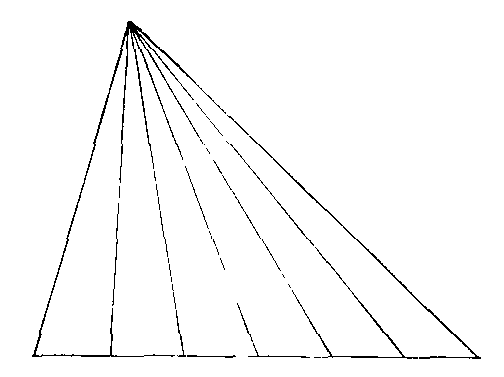
\includegraphics[width=40mm]{fig20.png}
\end{figure}

\textbf{証明.} 三角形は、一つの頂点から対辺上の点へ引いた線によって、不足あるいは過剰が等しく面積も等しい $n$ 個のより小さい三角形に分けることができる。これらの三角形の各々は、不足あるいは過剰がもとの三角形の不足あるいは過剰の $\frac{1}{n}$ であり、面積がもとの三角形の面積の $\frac{1}{n}$ である。

二つの三角形の不足あるいは過剰が通約できる、たとえば比が $m: n$ であるときは、それらを、それぞれ $m$ 個と $n$ 個の、すべて同じ不足あるいは過剰と同じ面積をもつより小さい三角形に分けることができる。与えられた三角形の面積は、したがって同じ比 $m : n$ をなす。

\begin{figure}[h]
\centering
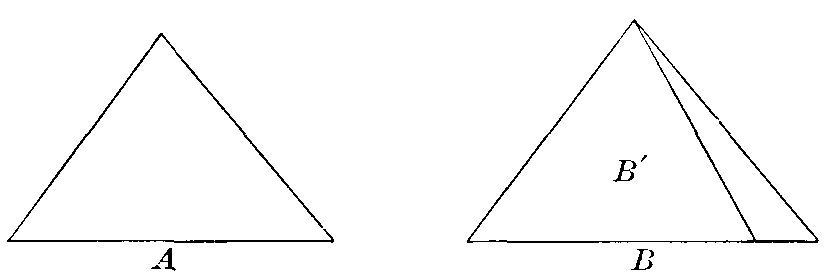
\includegraphics[width=70mm]{fig21.png}
\end{figure}

二つの三角形 $A$ と $B$ の不足あるいは過剰が通約できないときは、一方の三角形 $A$ を上のように任意の個数の等価な部分に分け、これらのうちの一つに等価な部分を、他方から、できるかぎり多くとる。すると、これらの部分の一つの不足あるいは過剰より小さい不足あるいは過剰をもつ残りができる。第二の三角形からとった部分は三角形 $B'$ をなす。$A$ と $B'$ は、不足あるいは過剰が通約できるから、面積がそれらに比例する。そこで $A$ を分ける部分の個数を限りなく増す。これらの部分は限りなく小さくなり、$B$ から $B'$ をとった残りも限りなく小さくなる。$B'$ の不足あるいは過剰と面積は、$B$ のそれらに近づき、三角形 $A$ と $B$ の面積は、それらの不足あるいは過剰に比例する。

\textbf{系.} \emph{二つの多角形の面積の比は、それらの不足あるいは過剰の比に等しい。}

\item[10.~定理.] \emph{一つの角を固定した直角三角形において、三角形の辺を限りなく小さくしてゆくとき、斜辺に対する対辺の比と斜辺に対する隣辺の比は、その角の正弦と余弦に極限として近づく。}

\textbf{証明.} 斜辺上に、任意個の等しい長さをとる。分点 $A_1$、$A_2$、$\cdots$ を通って底辺に垂線 $A_1C_1$、$A_2C_2$、$\cdots$ を引き、これらの線の延長に対して、斜辺の次の分点からそれぞれ垂線 $A_2D_1$、$A_3D_2$、$\cdots$ を引く。

三角形 $OA_1C_1$ と $A_2A_1D_1$ は等しい（II, 6, 系）。
\begin{align*}
  C_2A_2 &\gtrless C_1D_1 &&\text{かつ} & C_1C_2 &\lessgtr D_1A_2;\\
  \intertext{したがって、}
  \frac{C_2A_2}{OA_2} &\gtrless \frac{C_1A_1}{OA_1}
  &&\text{かつ} & \frac{OC_2}{OA_2} &\lessgtr \frac{OC_1}{OA_1},
\end{align*}
上側の符号は第二の仮説、下側の符号は第三の仮説に対応する。

\begin{figure}[h]
\centering
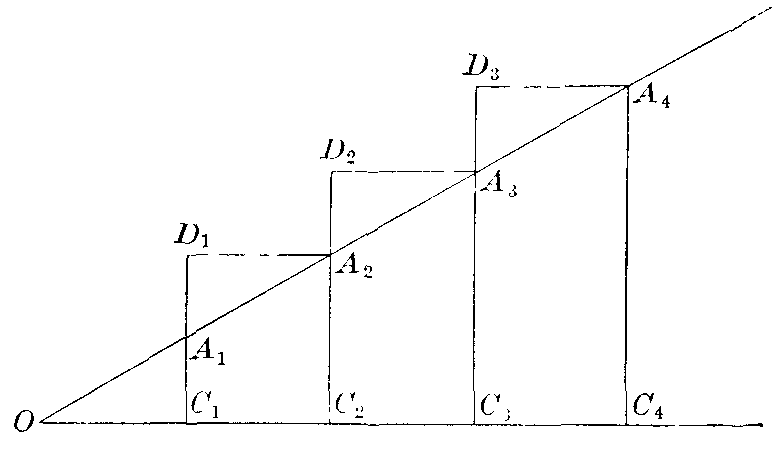
\includegraphics[width=70mm]{fig22.png}
\end{figure}

つぎを仮定する。
\begin{equation*}
  \frac{C_{r-1}A_{r-1}}{OA_{r-1}}
  \gtrless \frac{C_{r-2}A_{r-2}}{OA_{r-2}}
  \gtrless \dots
  \gtrless \frac{C_1A_1}{OA_1},
\end{equation*}
および
\begin{equation*}
  \frac{OC_{r-1}}{OA_{r-1}}
  \lessgtr \frac{OC_{r-2}}{OA_{r-2}}
  \lessgtr \dots
  \lessgtr \frac{OC_1}{OA_1}.
\end{equation*}

\begin{align*}
  OA_{r-1} &= (r-1) OA_1,\\
\intertext{かつまた}
           &= (r-1) A_{r-1}A_r,
\end{align*}
であるから、不等式
\begin{equation*}
  \frac{OC_1}{OA_1} \gtrless \frac{OC_{r-1}}{OA_{r-1}} \quad
  \text{および}\quad
  \frac{C_1A_1}{OA_1} \lessgtr \frac{C_{r-1}A_{r-1}}{OA_{r-1}}
\end{equation*}
を $A_{r-1}$ での角に適用すると、
\begin{equation*}
  \frac{A_{r-1}D_{r-1}}{A_{r-1}A_r} \gtrless
  \frac{C_{r-1}A_{r-1}}{OA_{r-1}}\quad
  \text{および}\quad
  \frac{D_{r-1}A_r}{A_{r-1}A_r} \lessgtr
  \frac{OC_{r-1}}{OA_{r-1}}
\end{equation*}
となる。

この二つの不等式のうち第一のものは、つぎのように書ける。
\begin{equation*}
  \frac{A_{r-1}D_{r-1}}{C_{r-1}A_{r-1}} \gtrless
  \frac{A_{r-1}A_r}{OA_{r-1}}.
\end{equation*}

両辺に 1 を加えると、
\begin{align*}
\frac{C_{r-1}D_{r-1}}{C_{r-1}A_{r-1}} &\gtrless
                                            \frac{OA_r}{OA_{r-1}}, \\
\intertext{すなわち}
\frac{C_{r-1}D_{r-1}}{OA_r} &\gtrless
                                   \frac{C_{r-1}A_{r-1}}{OA_{r-1}}, \\
\intertext{しかるに}
C_rA_r &\gtrless C_{r-1}D_{r-1}, \\
\intertext{したがって}
\frac{C_rA_r}{OA_r} &\gtrless \frac{C_{r-1}A_{r-1}}{OA_{r-1}}, \\
\end{align*}

またさらに、
\begin{align*}
C_{r-1}C_r &\lessgtr D_{r-1}A_r. \\
\intertext{ゆえに、上の第二の不等式から、}
\frac{C_{r-1}C_r}{A_{r-1}A_r} &\lessgtr \frac{OC_{r-1}}{OA_{r-1}}, \\
\intertext{すなわち}
\frac{C_{r-1}C_r}{OC_{r-1}} &\lessgtr \frac{A_{r-1}A_r}{OA_{r-1}}. \\
\end{align*}

両辺に 1 を加えると、
\begin{align*}
\frac{OC_r}{OC_{r-1}} &\lessgtr \frac{OA_r}{OA_{r-1}}, \\
\intertext{すなわち}
\frac{OC_r}{OA_r} &\lessgtr \frac{OC_{r-1}}{OA_{r-1}}
\end{align*}
となる。

比 $\dfrac{CA}{OA}$ と $\dfrac{OC}{OA}$ は 1 より小さく、斜辺が減少するとき、つねに増加するかつねに減少するから、確定した極限に近づく。これらの極限は $A$ の連続関数である。実際、任意の直角三角形の角を連続的に変化させ、斜辺をある一定の長さに保つと、他の二辺は連続的に変化するから、斜辺に対するそれらの比の極限も、連続的に変化しなければならない。

これらの極限をさしあたり $sA$ と $cA$ と呼ぶことにして、三角法でのように、その定義を任意の角に拡張し、正弦と余弦の公式がすべてこれらの関数についても成り立つことを証明できる。そして、特定の角 $30^\circ$、$45^\circ$、$60^\circ$ について、それらが正弦と余弦と同じ値をもつことを証明でき、他のすべての角でのそれらの値は、これらの角での値から定まるから、正弦と余弦の対応する値と同じになる。

\begin{figure}[ht]
\centering
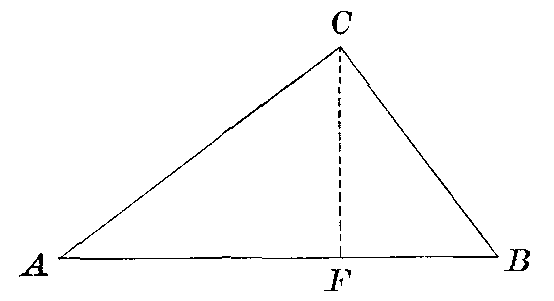
\includegraphics[width=50mm]{fig23.png}
\end{figure}

直角 $C$ から斜辺 $AB$ へ垂線 $CF$ を引く。角 $FCB$ は $A$ に等しくないが、その差は、二つの三角形 $ABC$ と $FBC$ の面積の差に比例するから、三角形の辺が小さくなるとき限りなく小さくなる。関係
\begin{equation*}
\frac{AF}{AC}\cdot\frac{AC}{AB} +
    \frac{FB}{BC}\cdot\frac{BC}{AB} = 1
\end{equation*}
から、極限へ移ると、
\begin{equation*}
(cA)^2 + (sA)^2 = 1
\end{equation*}
を得る。

$x$ と $y$ を任意の二つの鋭角とし、二つの角の和の正弦と余弦の公式を証明するのに用いる図を描く。

角 $x$ と $y$ を固定したまま、すべての線を限りなく小さくすることを考えることができ、関数 $sx$、$cx$、$sy$ などは、これらの線のある比の極限である。
\begin{gather*}
\begin{aligned}
\frac{CA}{OA} &= \frac{CE}{OB}\cdot\frac{OB}{OA}
                                + \frac{EA}{BA}\cdot\frac{BA}{OA}, \\
\pm \frac{CA}{OA} &= \frac{OD}{OB}\cdot\frac{OB}{OA}
                                - \frac{CD}{BA}\cdot\frac{BA}{OA}, \\
\end{aligned} \\
\left(\text{第二の図では} -\frac{OC}{OA} \right).
\end{gather*}

二つの三角形 $EMB$ と $CMO$ では $M$ での角が等しく、つぎのように書ける。
\begin{equation*}
\frac{CM}{OM} = \frac{ME + \delta}{MB}
                              = \frac{ME \pm CM + \delta}{MB \pm OM},
\end{equation*}
ここで $\delta$ の極限は零である。
\begin{equation*}
\therefore \lim \frac{CE}{OB} = \lim\frac{CM}{OM} = sx.
\end{equation*}

\begin{figure}[h]
\centering
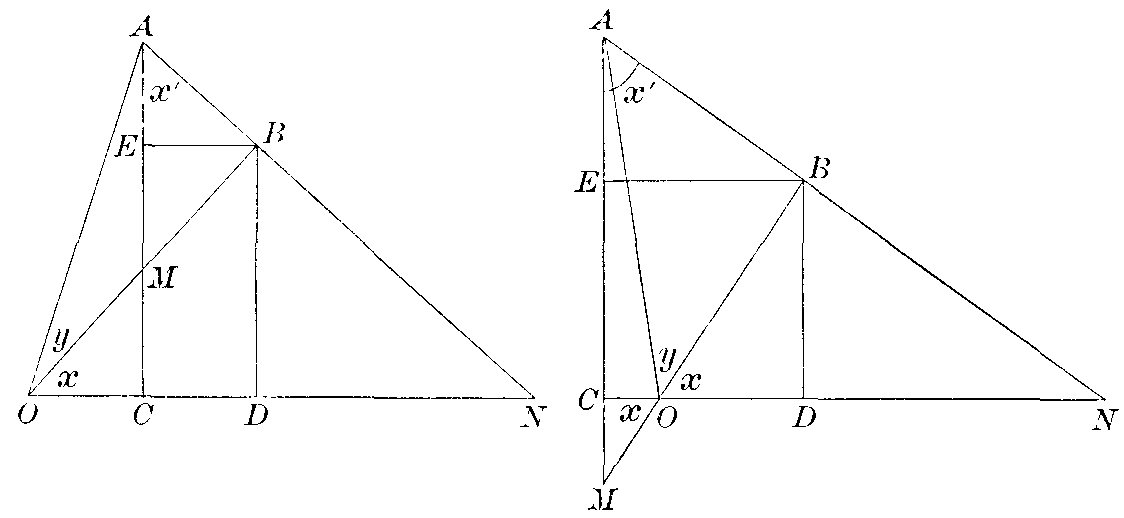
\includegraphics[width=80mm]{fig24.png}
\end{figure}

角 $EAB$、すなわち $x'$ は $x$ と同じではないが、$x$ との差は、三角形 $OMC$ と $MAB$ の面積の差に比例する量にすぎず、したがって限りなく小さくなる。こうして $sx'$ と $cx'$ の極限は $sx$ と $cx$ である。

最後に、二つの三角形 $ACN$ と $BDN$ が角 $N$ を共有するから、つぎのように書ける。
\begin{equation*}
\frac{DN}{BN} = \frac{CN + \delta '}{AN}
                                = \frac{CN - DN + \delta '}{AN - BN},
\end{equation*}
ここで $\delta'$ の極限は零である。
\begin{equation*}
\therefore \lim \frac{CD}{AB} = \lim\frac{CN}{AN} = sx.
\end{equation*}

さて極限において、恒等式は
\begin{align*}
s(x+y) &=  sx \cdot cy + cx \cdot sy, \\
c(x+y) &=  cx \cdot cy - sx \cdot sy
\end{align*}
となる。

帰納法によって、これらの公式は任意の角について真であることが証明される。これらの関数の値を $30^\circ$、$45^\circ$、$60^\circ$ での値から計算するのに十分な他の公式は、この二つから代数的な操作で得られる。

直角二等辺三角形の辺が限りなく小さくなるとき、角は固定されたままではなく $45^\circ$ に近づき、斜辺に対する二辺の比は、極限 $s\ 45^\circ$ と $c\ 45^\circ$ に近づく。したがって、これらは等しく、それらの平方の和は 1 であるから、それぞれの値は $\frac{1}{\sqrt{2}}$ であり、$45^\circ$ の正弦と余弦の値と同じである。

また、正三角形を二等分して、斜辺が一辺の二倍となる三角形をつくる。この関係を保ったまま辺を小さくしてゆくと、角は $30^\circ$ と $60^\circ$ に近づく。したがって、これらの角の関数 $s$ と $c$ の値は、同じ角の正弦と余弦の対応する値と同じである。

\textbf{系.} \emph{平面三角形が限りなく小さくなるとき、辺と角の関係は、われわれになじみのある通常の幾何学と三角法の平面三角形の辺と角の関係に近づく。}

\item[11.~定理.] \emph{球面幾何学は三つの仮説において同じであり、球面三角法の公式は通常の球面三角法のものとまったく同じである。}

\textbf{証明.} 球面上では、大円の弧は、それが中心に対する角に比例し、球面上の角は、その角の辺である大円の平面がなす二面角に等しい。それらの関係は、望むだけ小さくできる、したがって直角の仮説における平面三角形のようであると仮定してよい、ある平面三角形を描くことによって確立される。ゆえに、これらの関係は通常の球面三角法のものである。
\end{description}

\medskip 三つの仮説は、三つの幾何学の体系を生じ、それらは放物幾何学、双曲幾何学、楕円幾何学と呼ばれる。これらはまた、ユークリッドの幾何学、ロバチェフスキーの幾何学、リーマンの幾何学とも呼ばれる。次のような考察は、それらの主な特徴のいくつかを示す。

\begin{figure}[h]
\centering
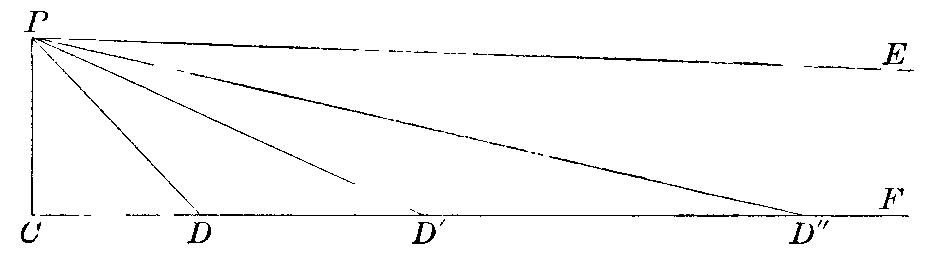
\includegraphics[width=80mm]{fig25.png}
\end{figure}

直線 $CF$ に垂直な $PC$ が与えられたとする。この直線上に、
\begin{align*}
  CD    &= PC, \\
  DD'   &= PD, \\
  D'D'' &= PD',\ \text{など}
\end{align*}
をとる。

さて $PC$ が十分に短い（限定されている）ならば、それは $P$ から直線 $CF$ に至る\emph{他のどんな}線よりも短い。なぜなら、$PC$ 以下の短さの線はどれも、点 $P$ のまわりの平面の限定された部分に含まれ、その部分では、垂線が点から直線への最短距離だからである。

したがって、
\begin{align*}
  PD  &> PC,               &\therefore CD' &> 2CD,\\
  PD' &> PC,\ \text{など;} &          CD'' &> 3CD,\ \text{など}
\end{align*}

またさらに、三つの仮説において、それぞれ、
\begin{align*}
  CPD    &\stackrel{=}{\lessgtr} \frac{\pi}{4}, &&\text{かつ}&
                         CDP &\stackrel{=}{\lessgtr} \frac{\pi}{4},\\
  DPD'   &\stackrel{=}{\lessgtr} \tfrac{1}{2} CPD, &&&
                    CD'P  &\stackrel{=}{\lessgtr} \tfrac{1}{2} CDP,\\
  D'PD'' &\stackrel{=}{\lessgtr} \tfrac{1}{2} DPD',\ \text{など,} &&&
        CD''P &\stackrel{=}{\lessgtr} \tfrac{1}{2} CD'P,\ \text{など}
\end{align*}

$P$ には一連の角ができる。第一の仮説では、これらの角は無限に多くあり、その列は公比 $\frac{1}{2}$ の等比数列をなし、その和はちょうど $\frac{\pi}{2}$ である。第二の仮説でも、これらの角は無限に多くあり、列の各項は等比数列の各項より小さい。したがって、その列の和は $\frac{\pi}{2}$ より小さい。第三の仮説では、各項が等比数列の各項より大きい列ができ、したがって、その列が収束するか発散するかにかかわらず、十分な数の項をとれば $\frac{\pi}{2}$ より大きくなる。いいかえれば、この過程を有限の回数くり返すことによって、$P$ に直角か、それより大きな角が得られる。

$D$、$D'$、$D''$、$\cdots$ での角は、$P$ での角の列の各項にちょうど等しい。最初の二つの仮説では、それらは極限として零に近づく。

距離 $CD$、$CD'$、$CD''$、$\cdots$ は、毎回、ある確定した量 $CD$ より多く増加する。したがって、この過程を限りなくくり返すと、これらの距離はあらゆる限界を超えて増大する。こうして、第一および第二の仮説では、直線が無限の長さをもたなければならないことが証明される。

鈍角の仮説では、$PC$ に点 $P$ で垂直な線は、$C$ から有限のある距離にある点、すなわち $D$ のどれか、またはその間のある点で、$CF$ と交わる。$PC$ の反対側でも、この同じ垂線は、延長した $FC$ と同じ距離のところで交わる。しかし、二つの異なる直線が二点で交わることはないと仮定してあるから、われわれにとって第三の仮説は、直線が有限の長さをもち、それ自身に戻る場合にのみ真でありうる。このとき、これら二つの点は同一の点であり、その $C$ からの距離は、どちらの向きでも直線全体の長さの半分である。しかし、このようにして、第三の仮説の上に無矛盾な幾何学を築くことができ、この幾何学が楕円幾何学と呼ばれるものである。

作図は、$CF$ 上に任意の長さの $CD$ をとっても同じであり、ほとんどすべての叙述も同じになったはずである。

この章の命題のいくつかに課した制限は、第三の仮説では必要である。

\begin{figure}[h]
\centering
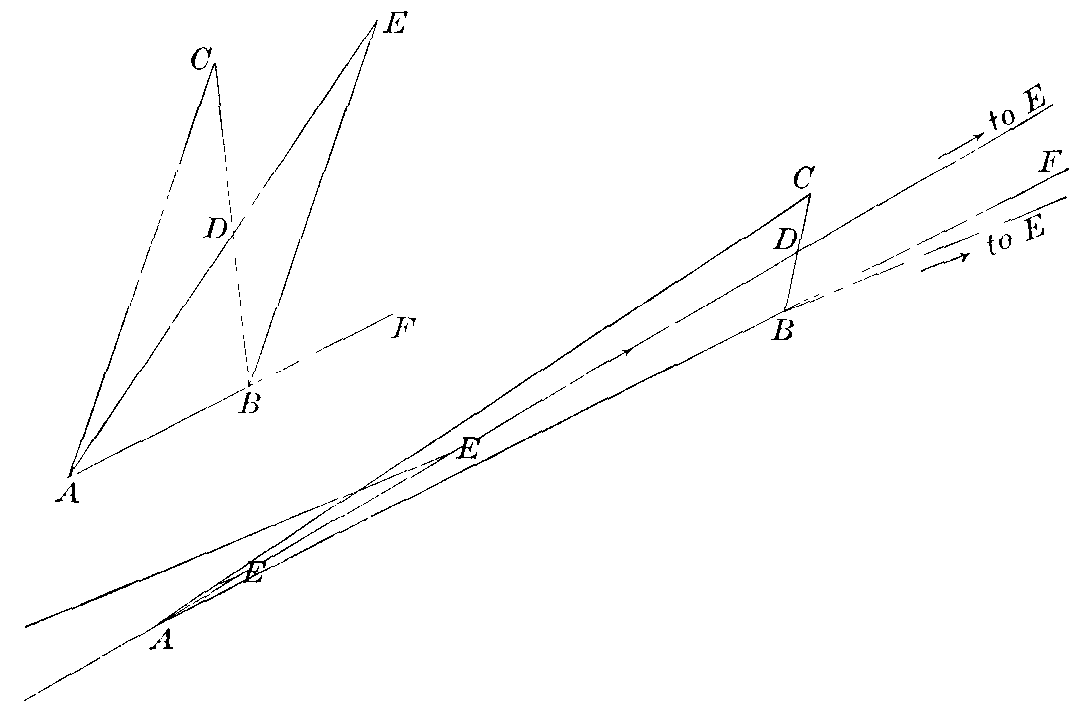
\includegraphics[width=80mm]{fig26.png}
\end{figure}

たとえば、三角形の外角が隣り合わない内角より大きいことの証明では、頂点 $A$ から対辺の中点 $D$ へ引いた線 $AD$ を、$AE=2AD$ となるように延長した。$AD$ が、$A$ と $D$ で定まる直線の全長の半分より大きければ、これは点 $E$ を点 $A$ の先へ持ってゆくことになり、角 $C$ に等しい角 $CBE$ は、外角 $CBF$ の一部となる代わりに、この外角より大きくなる。

\begin{figure}[h]
\centering
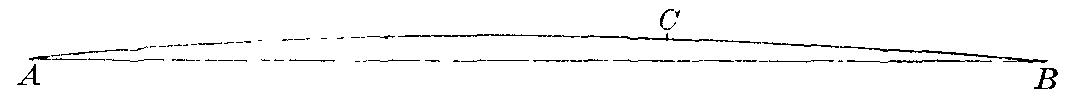
\includegraphics[width=80mm]{fig27.png}
\end{figure}

また、三角形の二つの角が等しく、その間の辺がちょうど直線全体であるときは、対辺が等しいことは必ずしも導かれない。しかし、その対辺は一つの連続した線をなすのだから、この図形は厳密には三角形ではなく、むしろ月形に似た図形であるともいえる。点 $A$ と $B$ は同じ点であり、角 $A$ と $B$ は対頂角である。

最後に、二点間の最短の道は直線であると仮定してはいるが、二点の間に引いた直線がつねにその二点間の最短の道であるとは限らない。直線上で一方の点から他方へ行く方法は二通りある。すなわち、二点がその決める直線を分けてできる二つの部分のそれぞれを通る道である。これらの部分の一方は通常は他方より短く、長いほうの部分は、折れ線や曲線に沿ったいくつかの道より長くなる。

しかし、直線が無限の長さをもつとき、すなわち直角の仮説と鋭角の仮説においては、この章の命題はすべて制限なしに成り立つ。

\medskip ユークリッド幾何学はだれにもなじみ深い。つぎにロバチェフスキーの幾何学を詳しく調べ、そのあと同じ方法で楕円幾何学を取り上げよう。


\chapter{双曲幾何学}

いま鋭角の仮説をとる。平面上で第三の直線に垂直な二直線は、その共通の垂線の両側で互いに離れてゆく。三角形の角の和は二直角より小さく、前章の命題は制限なしに成り立つ。

\section{平行線}

任意の点 $P$ から、与えられた直線 $AB$ へ垂線 $PC$ を引き、$P$ から $CB$ 上の点 $D$ へ別の線 $PD$ を引く。$D$ が $CB$ 上を限りなく遠ざかってゆくと、線 $PD$ はある極限の位置 $PE$ に近づく。

\begin{figure}[h]
\centering
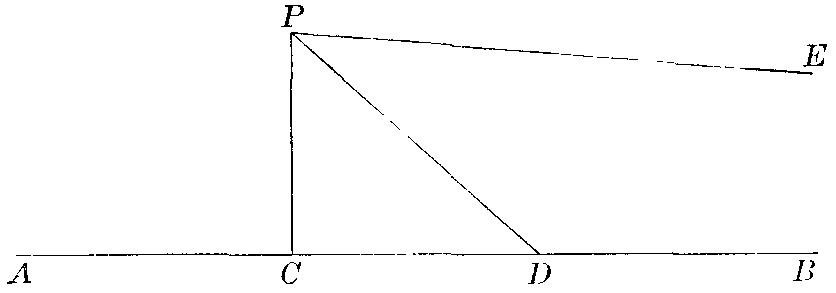
\includegraphics[width=80mm]{fig28.png}
\end{figure}

$PE$ は、$P$ において $CB$ に\emph{平行}であるという。$PE$ が $PC$ となす角 $CPE$ を、垂直距離 $PC$ に対する\emph{平行角}という。それは直角より小さく、小さい量は三角形 $PCD$ の不足の極限である。$PC$ の反対側にも、$CA$ に平行で、$PC$ と同じ平行角をなす別の線を見いだすことができる。$PE$ は、$PC$ に関して $PE$ と同じ側にある部分に向かって $AB$ に平行であるという。このように、任意の点において、一つの直線に対する平行線は二本あるが、直線の一方の向きに対しては一本だけである。$P$ を通る線で、$PC$ とのなす角が平行角より大きく、かつその補角より小さいものは、$AB$ とまったく交わらない。垂直距離 $p$ に対する平行角を $\Pi(p)$ と書く。

\begin{description}
\item[1.~定理.] \emph{直線は、すべての点においてその平行性を保つ。}

\begin{figure}[h]
\centering
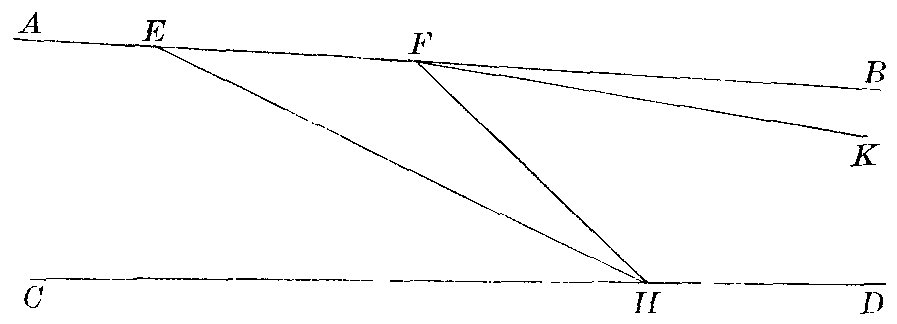
\includegraphics[width=80mm]{fig29.png}
\end{figure}

\textbf{$AB$} が $E$ において $CD$ に平行であるとし、$E$ の両側の $AB$ 上の任意の他の点を $F$ とするとき、$AB$ が $F$ においても $CD$ に平行であることを証明する。

\textbf{証明.} $CD$ 上の $H$ に、$EH$ と $FH$ を引く。$H$ が $CD$ 上を限りなく遠ざかると、これら二つの線は $CD$ に平行な位置に近づく。しかし $EH$ の極限の位置は、$F$ を通る直線 $AB$ であり、もし $FH$ の極限の位置が別の線 $FK$ であるとすれば、$F$ が、$EH$ と $FH$ の交点である $H$ の極限の位置になってしまう。

\item[2.~定理.] \emph{一つの直線が他の直線に平行ならば、第二の直線は第一の直線に平行である。}

\textbf{$AB$} が $CD$ に平行であるとき、$CD$ が $AB$ に平行であることを証明する。

\textbf{証明.} $CD$ に垂直に $AC$ を引く。角 $CAB$ は鋭角である。したがって、$C$ から $AB$ へ下ろした垂線 $CE$ は、直線 $AB$ が $CD$ に平行である向きの側の、$A$ の側に落ちなければならない（第I章, II, 1）。そのとき角 $ECD$ は鋭角で、直角である $CEB$ より小さい。すなわち、
\begin{equation*}
CAB < ACD, \quad \text{かつ} \quad CEB > ECD
\end{equation*}
である。

線 $CE$ が点 $C$ のまわりに $CA$ の位置まで回転すると、$E$ での角は角 $A$ まで減少し、$C$ での角は直角まで増加する。この二つの角が等しくなる位置が、たとえば $CF$ にある。すなわち、
\begin{equation*}
CFB = FCD
\end{equation*}
である。

\begin{figure}[h]
\centering
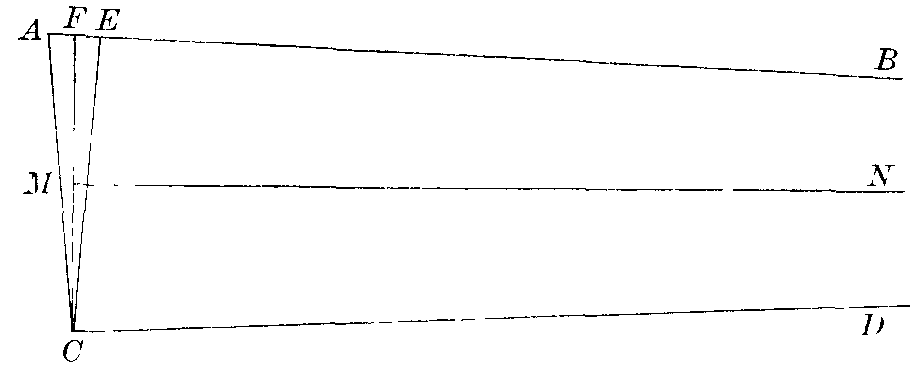
\includegraphics[width=80mm]{fig30.png}
\end{figure}

$CF$ の中点で $CF$ に垂直に $MN$ を引き、図形を $MN$ を軸として回転させる。$CD$ は $AB$ のもとの位置に重なり、$AB$ は $CD$ のもとの位置に重なる。したがって、$CD$ は $AB$ に平行である。

\textbf{系.} \emph{$FB$ と $CD$ は、ともに $MN$ に平行である。}

\begin{figure}[h]
\centering
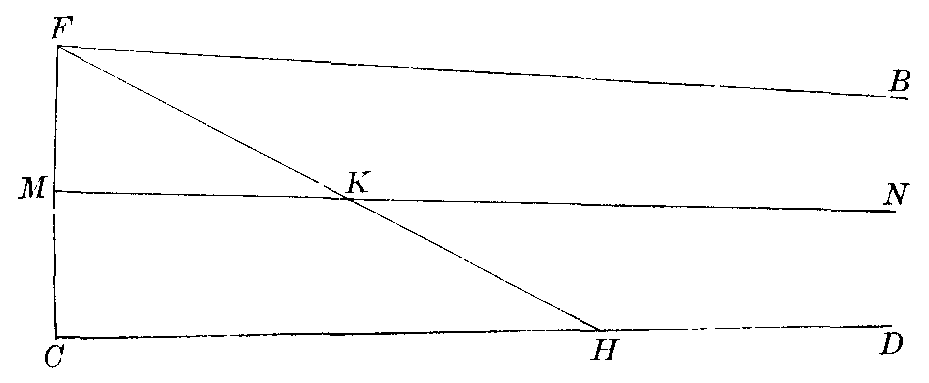
\includegraphics[width=80mm]{fig31.png}
\end{figure}

\textbf{証明.} $FB$ と $CD$ は $MN$ に関して対称の位置にあり、互いに交わらないから、$MN$ とも交わらない。$CD$ 上の $H$ に $FH$ を引き、$MN$ と $K$ で交わるとする。$H$ が $CD$ 上を限りなく遠ざかると、$FH$ は極限として $FB$ の位置に近づく。ところで、$K$ が $H$ より先に限りなく遠ざかることはできない。$FK < FH$ だからである。しかしまた、$H$ が限りなく遠ざかるとき、$K$ が $MN$ 上の有限の距離にある極限の位置に近づくこともできない。そうなれば、$FB$、したがって $CD$ は、この点で $MN$ と交わり、互いにも交わることになるからである。ゆえに $H$ と $K$ は一緒に遠ざからなければならず、$FH$ の極限の位置は、同時に $CD$ と $MN$ に平行でなければならない。

同様にして、平面上で二本の平行線の間にある任意の線は、そのどちらかと交わるか、両方に平行であることを証明できる。

\item[3.~定理.] \emph{第三の直線の同じ向きに対してそれに平行な二直線は、互いに平行である。}

\begin{figure}[h]
\centering
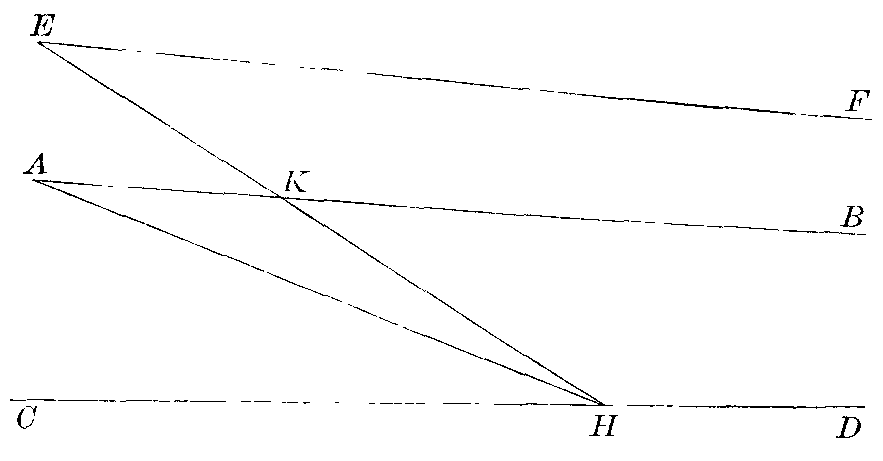
\includegraphics[width=80mm]{fig32.png}
\end{figure}

\textbf{第一に、}すべてが同じ平面にあるとき。

\textbf{$AB$} と $EF$ が $CD$ に平行であるとき、それらが互いに平行であることを証明する。

\textbf{証明.} $AB$ が他の二直線の間にあるとする。$CD$ 上の任意の点 $H$ に $AH$ と $EH$ を引き、$EH$ が $AB$ と交わる点を $K$ とする。$H$ が $CD$ 上を限りなく遠ざかるとき、$AH$ と $EH$ は極限の位置として $AB$ と $EF$ に近づく。ところで、$K$ が $H$ より先に限りなく遠ざかることはできない。$EK < EH$ だからである。しかしまた、$H$ が限りなく遠ざかるとき、$K$ が $AB$ 上の有限の距離にある極限の位置に近づくこともできない。この点は $AB$ と $EF$ の交点であり、$H$ の極限の位置でもあることになるが、$H$ は $CD$ 上を限りなく遠ざかるからである。ゆえに $H$ と $K$ は一緒に遠ざからなければならず、$EH$ の極限の位置は同時に $CD$ と $AB$ に平行でなければならない。

他の二直線の間にある $AB$ が、$CD$ と $EF$ に平行であると与えられているならば、$EF$ は $CD$ に平行でなければならない。$E$ を通って $CD$ に平行な線は $AB$ に平行であり、同じ向きに対して $E$ を通って $AB$ に平行な線は一本しか引けないからである。

\begin{figure}[h]
\centering
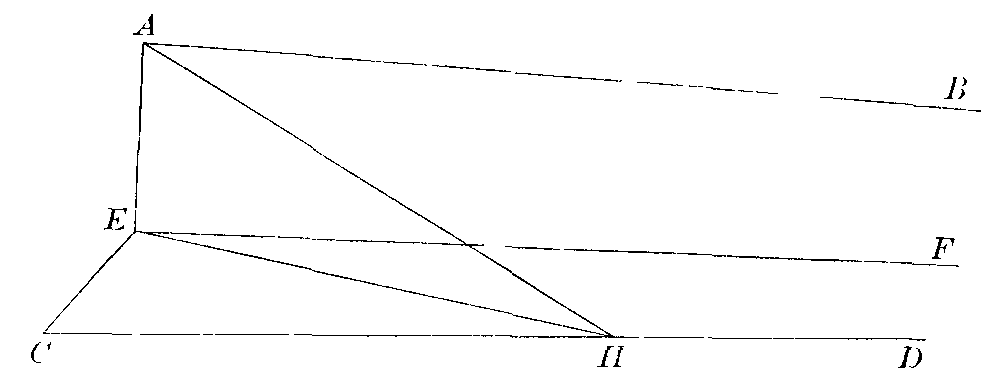
\includegraphics[width=80mm]{fig33.png}
\end{figure}

\textbf{第二に、}直線がすべて同じ平面にないとき。

\textbf{$AB$} と $CD$ を二本の平行線とし、$E$ をそれらの平面にない任意の点とする。

\textbf{証明.} $CD$ 上の $H$ に、$AH$ と $EH$ を引く。$H$ が限りなく遠ざかるとき、$AH$ は $AB$ の位置に近づき、平面 $EAH$ は平面 $EAB$ の位置に近づく。したがって、$EH$ の極限の位置は平面 $ECD$ と $EAB$ の交線である。そうするとこれらの平面の交線は $CD$ に平行であり、同様にして、それが $AB$ にも平行であることが証明される。

さて、$EF$ がこの二直線の一方に、それらが平行である向きに対して平行であると与えられているならば、それは、それらと点 $E$ とによって定まる二つの平面の交線でなければならず、したがって他方の直線にも平行である。

\item[4.~定理.] \emph{平行線は互いに近づきつづける。}

\textbf{$AB$} と $CD$ が平行であるとし、$AB$ 上の任意の点 $A$ と $B$ から、$CD$ へ垂線 $AC$ と $BD$ を下ろす。$B$ が平行の向きに関して $A$ の先にあるとして、$BD < AC$ を証明する。

\textbf{証明.} $CD$ の中点 $H$ に、$AB$ と $K$ で交わる垂線を立てる。角 $BKH$ は鋭角であり、角 $AKH$ は鈍角である。したがって、$K$ で $HK$ に垂直な線は、$CA$ と $C$ と $A$ の間のある点 $E$ で、延長した $DB$ と $B$ の先のある点 $F$ で交わらなければならない。しかるに $DF = CE$（第I章, I, 12）であるから、$DB < CA$ である。

\begin{figure}[h]
\centering
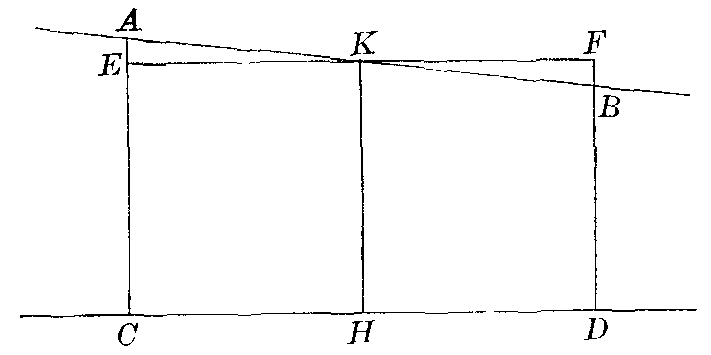
\includegraphics[width=80mm]{fig34.png}
\end{figure}

\textbf{系.} \emph{$AB$ と $CD$ が平行で、$AC$ がそれらと等しい角をなす（上の 2 の $FC$ のような）ならば、この二直線上に等しい距離 $AE = CF$ を、それらが平行である向きの側に切り取る $EF$ は、$AC$ より短い。}

\begin{figure}[h]
\centering
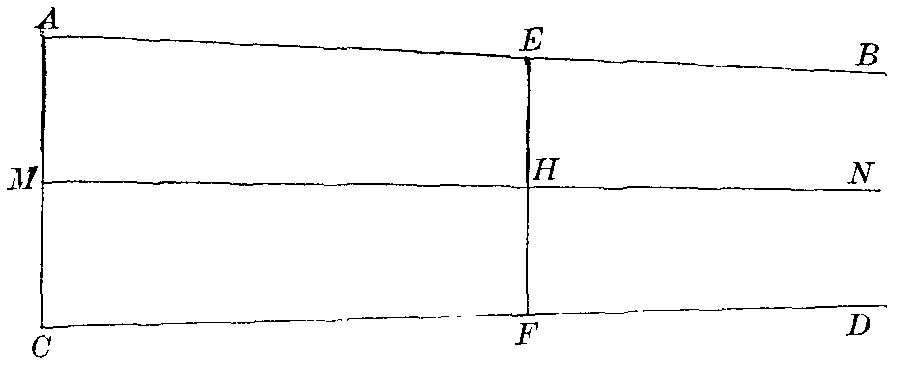
\includegraphics[width=80mm]{fig35.png}
\end{figure}

\textbf{証明.} $AC$ の中点で $AC$ に垂直な $MN$ は、$AB$ に平行で、$EF$ を二等分する。図形は $MN$ に関して対称だからである。$EF$ の半分である $EH$ は $AM$ より小さく、したがって $EF$ は $AC$ より小さい。

\item[5.~定理.] \emph{垂直距離が零から出発して限りなく増加するとき、平行角は直角から零まで減少する。}

\textbf{証明.} まず第一に、平行角は、垂直距離が正である間は鋭角であるが、垂直距離を十分に小さくとれば、直角との差をどんな指定された値よりも小さくできる。

\begin{figure}[ht]
\centering
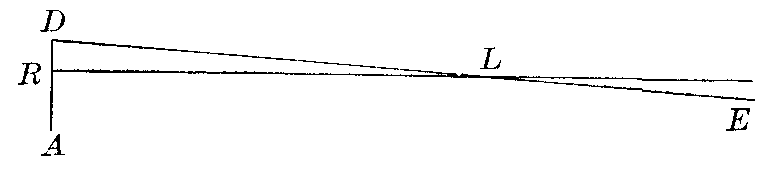
\includegraphics[width=70mm]{fig36.png}
\end{figure}

実際、$ADE$ を、望むだけ直角に近い任意の角とするとき、$DE$ 上に点 $L$ をとり、$LR$ を $R$ で $DA$ に垂直に引くことができる。角 $RDL$ は、増加して、垂直距離 $RD$ に対する平行角となる。

\begin{figure}[h]
\centering
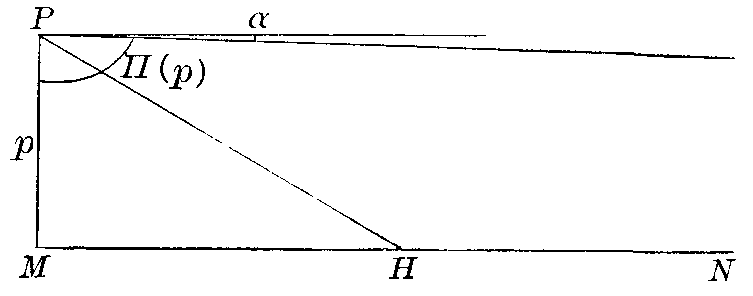
\includegraphics[width=70mm]{fig37.png}
\end{figure}

つぎに、$p$ を与えられた垂線 $PM$ の長さとし、$\alpha$ を、その平行角が $\frac{\pi}{2}$ と異なる量とする。すなわち、
\begin{equation*}
\Pi(p) = \frac{\pi}{2} - \alpha
\end{equation*}
とおく。$PM$ が $MN$ に垂直で、$H$ が $MN$ 上の任意の点であるとき、$H$ が $MN$ 上を限りなく遠ざかると、角 $MPH$ は極限として平行角 $\Pi(p)$ に近づく。線 $PH$ は、$MPH < \Pi(p)$ の間は線 $MN$ と交わり、$MPH$ を $\Pi(p)$ に十分近く、しかしそれより小さくとることによって、角 $MHP$ を望むだけ小さくできる（前章の該当ページを見よ）。

次ページの図（図38）において、$AC$ を $AB$ に垂直とし、$D$ を $AC$ 上の任意の点、$DE$ を $AB$ に平行な線とする。$DE$ の先に $DK$ を引き、$DE$ と角 $EDK=\Pi(p)$ をなすようにし、$DK = p$ とする。$K$ で $DK$ に垂直な $TF$ は、$DE$ と $AB$ に平行になる。

前の図の $PM$ を $DKT$ の上に置くことにより、
\begin{gather*}
KDC < \Pi(p), \\
\intertext{すなわち}
ADE > 2\alpha
\end{gather*}
ならば、$DC$ は $KT$ と点 $G$ で交わることがわかる。

そのとき直角三角形 $DKG$ において、
\begin{gather*}
DGK + KDG < \frac{\pi}{2}. \\
\intertext{しかるに}
ADE + KDG = \frac{\pi}{2} + \alpha; \\
\intertext{したがって、}
DGK < ADG - \alpha.
\end{gather*}

\begin{figure}[h]
\centering
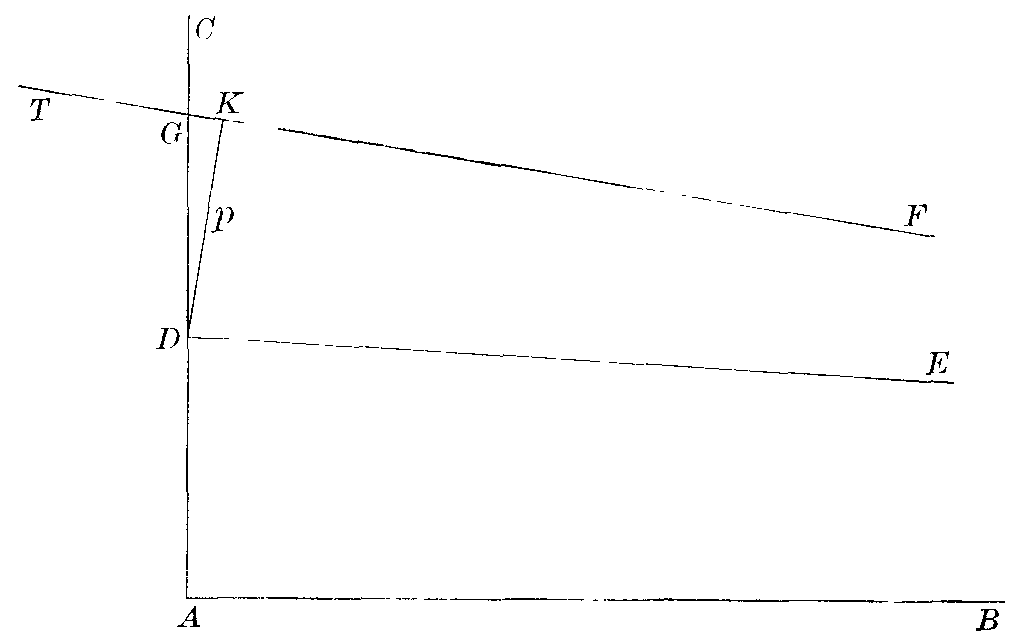
\includegraphics[width=80mm]{fig38.png}
\end{figure}

点 $G$ から出発して、この作図をくり返すことができ、そのたびに平行角から $\alpha$ より大きい量を引く。この過程は、平行角が $2\alpha$ に等しいか、それより小さくなるまで続けることができる。

点 $D$ が $AC$ に沿って動き、$DE$ が $AB$ に平行であるままならば、$D$ での角は絶えず減少し、$D$ を $AC$ に沿って十分遠くまで動かすことによって、この角が $2\alpha$ に等しいか、それより小さくなる点に達することができる。

$D$ が、平行角がちょうど $2\alpha$ となる点にあるとする。そこで、前と同様に $DK$ と $TF$ を引くと、$KT$ は $DC$ に平行になる。$AB$ とこの位置の $TF$ との間にある $AB$ へのすべての平行線は $AC$ と交わり、平行線がこの位置の $TF$ に近づくにつれて、$D$ での平行角は零に近づき、点 $D$ は限りなく遠ざかる。

\begin{figure}[h]
\centering
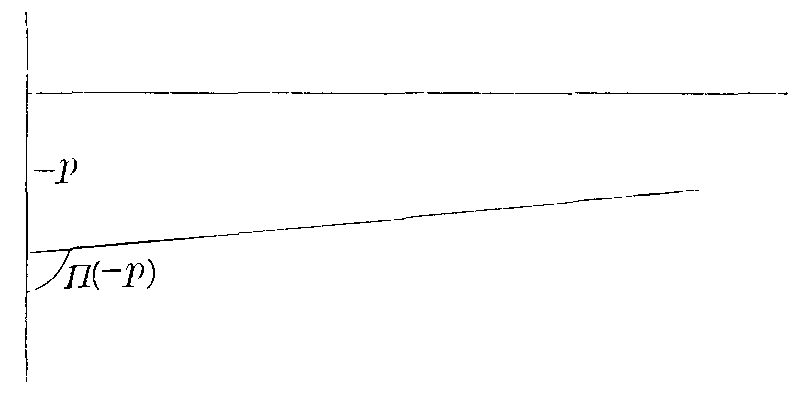
\includegraphics[width=60mm]{fig39.png}
\end{figure}

鈍角については、$p$ を負にとることができて、
\begin{equation*}
\Pi(-p) = \pi - \Pi(p)
\end{equation*}
である。


\item[6.~定理.] \emph{三角形の各辺の中点に立てた垂線は、そのうち二本が平行ならば、すべて平行である。}

\begin{figure}[h]
\centering
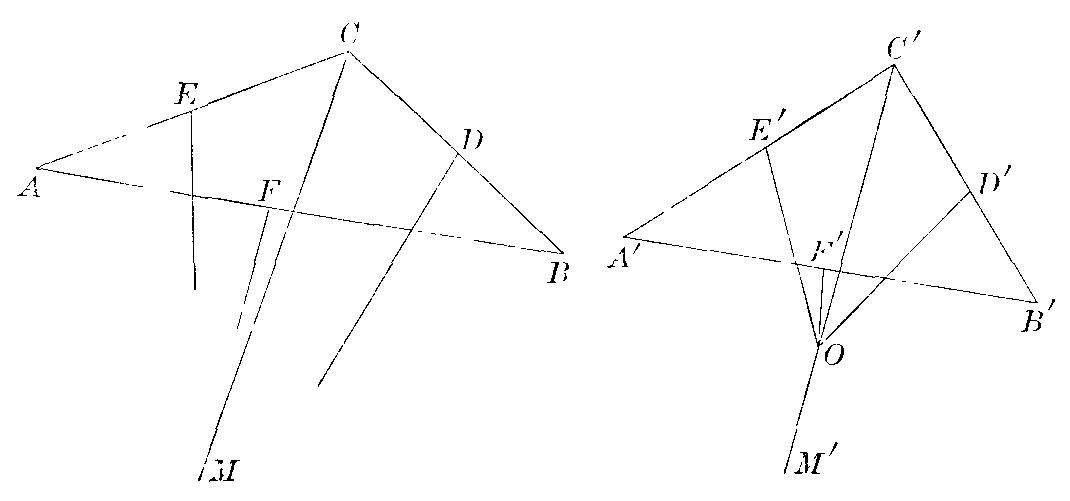
\includegraphics[width=90mm]{fig40.png}
\end{figure}

\textbf{$A$}、$B$、$C$ を三角形の頂点とし、$D$、$E$、$F$ をそれぞれの対辺の中点とする。$D$ と $E$ での垂線が平行であると与えられているとき、$F$ での垂線もそれらに平行であることを証明する。

\textbf{証明.} 与えられた二本の平行な垂線に平行に、$C$ を通る $CM$ を引く。$CM$ は、$C$ の二辺とのあいだに平行角 $\Pi\left(\dfrac{a}{2}\right)$ と $\Pi\left(\dfrac{b}{2}\right)$ をなし、$C$ での角はこれらの和または差である。和になるのは $C$ が与えられた垂線の間にあるとき、差になるのは $C$ が両方の同じ側にあるときである。$CA$ と $CB$ の長さを変えずに、$C$ でのこれらの角を適当に小さくすることによって、それらの中点 $D$ と $E$ での垂線が、$C$ から $\frac{a}{2}$ より大きく、かつ $\frac{b}{2}$ より大きい任意の距離のところで、$CM$ と、したがって互いに、交わるようにできる。

こうしてできた三角形を $A'B'C'$ とし、与えられた二本の垂線が交わる点を $O$、$O$ を通る線を $C'M'$ とする。三角形 $A'B'C'$ では、三本の垂線は点 $O$ で交わる（第I章, I, 5）。さて、作図をそのままにして、$O$ を $C'M'$ 上で遠ざけることができる。すなわち、線 $C'A'$ と $C'B'$ を、長さを変えずに $C'$ のまわりに回転させ、三本の垂線 $D'O$、$E'O$、$F'O$ がつねに $O$ を通るようにする。$O$ が限りなく遠ざかるとき、$C'$ での角は極限として $\Pi\left(\dfrac{a}{2}\right)$ と $\Pi\left(\dfrac{b}{2}\right)$ に近づき、三本の垂線は、$C'M'$ に、また互いに、平行な位置に近づく。しかし三角形 $A'B'C'$ は、極限として、二辺とその間の角がそれぞれ $ABC$ の対応する部分に等しい三角形、すなわち $ABC$ に等しい三角形に近づく。ゆえに $ABC$ では、三本の垂線はすべて平行である。

\item[7.~定理.] \emph{交わらず、平行でもない二直線は、ただ一つの共通垂線をもつ。}

\textbf{証明.} $AB$ と $CD$ をその二直線とし、$AB$ の任意の点 $A$ から $CD$ に垂線 $AC$ を下ろす。$AC$ 自身が共通垂線でなければ、$AC$ が $AB$ となす角の一方は鋭角である。この角が $AB$ の側にあるとして、$BAC < \frac{\pi}{2}$ とする。$AC$ の同じ側に、$CD$ に平行に $AE$ を引く。$AB$ は $CD$ に平行でもなく交わりもしないから、角 $EAC$ は $BAC$ より小さい。角 $EAC$ の内部に任意の線 $AH$ を引き、$CD$ と $H$ で交わらせる。$H$ が $C$ の位置から出発して線 $CD$ 上を限りなく遠ざかるならば、角 $BAH$ は角 $BAC$ の大きさから角 $BAE$ まで減少する。角 $AHC$ は、$BAC$ より大きい直角である $C$ での角の大きさから、\emph{限りなく}減少する。したがって $BAH=AHC$ となる位置がある。この位置では、$AH$ の中点を通って与えられた二直線の一方に垂直な線 $NM$ は、第I章, I, 10 で証明したように、他方にも垂直である。

\begin{figure}[h]
\centering
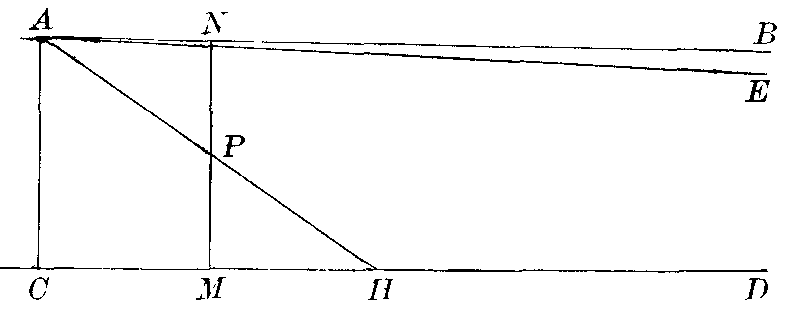
\includegraphics[width=80mm]{fig41.png}
\end{figure}

共通垂線が二本あれば長方形ができるが、それは双曲幾何学では不可能である。

\item[8.~定理.] \emph{三角形の各辺の中点に立てた垂線が、交わらず、平行でもないならば、それらはすべてある直線に垂直である。}

\begin{figure}[h]
\centering
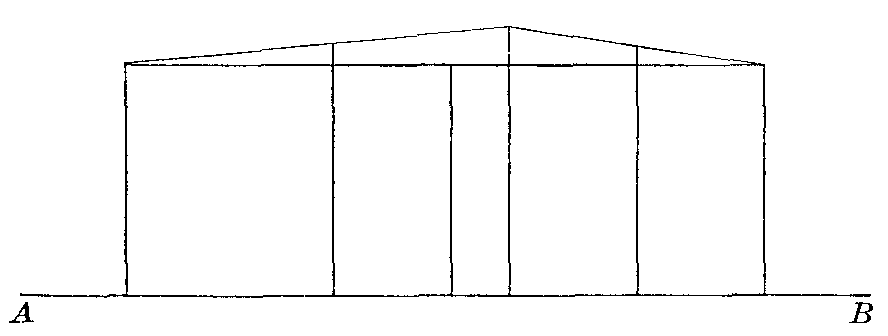
\includegraphics[width=90mm]{fig42.png}
\end{figure}

\textbf{証明.} これらの線のうち二本に垂直な線 $AB$ を引くことができ、第I章, II, 13 により、三角形の三つの頂点からこの線へ下ろした垂線は等しい。これら三つのうちの任意の二つの中間に立てた $AB$ への垂線は、三角形の対応する辺に対して、その中点で垂直である（第I章, I, 11）。こうして、三角形の各辺の中点に立てた三本の垂線はすべて $AB$ に垂直である。

直線は、平面への射影に平行であるとき、その平面に平行であるという。

\item[9.~定理.] \emph{平面にない任意の直線に対して、平面に垂直で、その直線に平行な線を引くことができる。}

\begin{figure}[h]
\centering
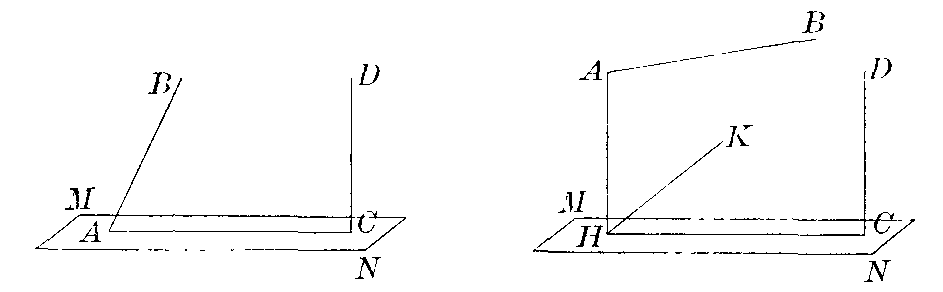
\includegraphics[width=100mm]{fig43.png}
\end{figure}

\textbf{証明.} $AB$ を与えられた直線、$MN$ を平面とする。$AB$ が平面 $MN$ と点 $A$ で出会うならば、その射影上に、$A$ での角が $\Pi(AC)$ に等しくなるような長さ $AC$ をとる。すると、$C$ で平面に垂直な $CD$ は $AB$ に平行になる。同様にして、平面の反対側にも、延長した $BA$ に平行な垂線を引くことができる。

$AB$ が $MN$ と出会わないならば、少なくとも一方の向きでは $MN$ から離れてゆく。平面上の $AB$ の射影の任意の点 $H$ を通って、$MN$ から離れてゆく $AB$ の部分に向かって、$AB$ に平行な線 $HK$ を引き、つぎにこの線に平行で平面に垂直な $CD$ を引くことができる。

$AB$ が $MN$ に平行でなければ、それは平面とどこかの点で出会うか、平面と線が共通垂線をもち、線が両方の向きで平面から離れてゆくかのいずれかである。後者の場合には、線に平行な垂線が二本あり、線の各部分に対して一本ずつ平行である。

二本の垂線が、線の同じ向きに対して平行であることはできない。そうなれば、それらは互いに平行になるが、平面に垂直で互いに平行な二直線は存在しないからである。
\end{description}

\section{限界曲線と限界面、等距離曲線と等距離面}

直線 $AB$ が与えられたとき、その端点 $A$ で任意の角をとり、辺 $AC$ を、その中点に立てた垂線が $AB$ に平行になるように延長する。点 $C$ の軌跡は、\emph{オリサイクル}あるいは\emph{限界曲線}と呼ばれる曲線である。$AB$ はその\emph{軸}である。

\begin{figure}[h]
\centering
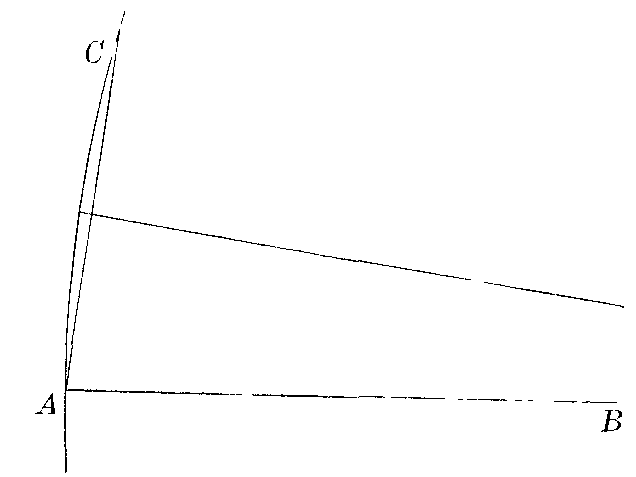
\includegraphics[width=60mm]{fig44.png}
\end{figure}

定義から、すべての限界曲線は等しく、限界曲線はその軸に関して対称である。すなわち、その軸のまわりに二直角だけ回転させると、それ自身に重なる。

\begin{description}
\item[1.~定理.] \emph{限界曲線の軸に平行な任意の線を軸にとることができる。}

\textbf{$AB$} を軸、$CD$ を $AB$ に平行な任意の線とし、$CD$ を軸にとれることを証明する。

\begin{figure}[h]
\centering
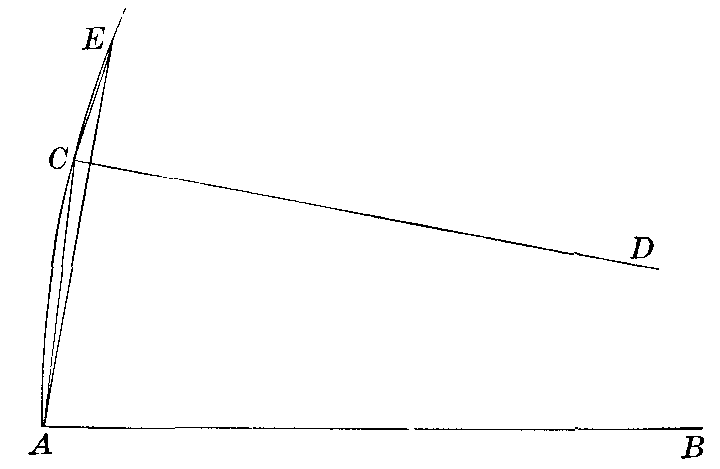
\includegraphics[width=70mm]{fig45.png}
\end{figure}

\textbf{証明.} $AC$ を引く。また、曲線上の任意の他の点 $E$ に、$AE$ と $CE$ を引く。$AC$ の中点と $AE$ の中点に立てた垂線は、$AB$ と $CD$ に、また互いに平行である。したがって、三角形 $ACE$ の第三辺 $CE$ の中点に立てた垂線は、それらに、また $CD$ に平行である。ゆえに $CD$ を軸にとることができる。

\textbf{系.} \emph{限界曲線は、形を変えずにそれ自身の上を滑らせることができる。すなわち、曲率が一定である。}

\item[2.~定理.] \emph{共通の軸の組をもつ二つの限界曲線は、軸のそれぞれの上に同じ距離を切り取り、対応する弧の比はこの距離だけに依存する。}

\begin{figure}[h]
\centering
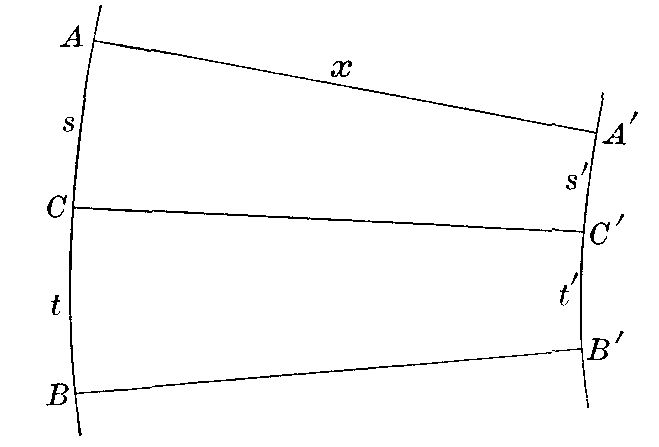
\includegraphics[width=70mm]{fig46.png}
\end{figure}

\textbf{証明.} 任意の二つの軸をとり、第三の軸が、最初の二つが二つの限界曲線の一方の上に切り取る弧を二等分するようにとる。図形をこの軸のまわりに回転させることによって、曲線が二つの軸の上に等しい距離を切り取ることが示される。

$AA'$、$BB'$、$CC'$ を、二つの限界曲線 $AB$ と $A'B'$ の任意の三つの軸とし、それらの共通の長さを $x$ とし、それらが $AB$ 上に弧 $s$ と $t$ を、$A'B'$ 上に $s'$ と $t'$ を切り取るとする。

$s = t$ のとき $s' = t'$ であり、一般に、
\begin{equation*}
\frac{s}{t} = \frac{s'}{t'}
\end{equation*}
である。これは、まず $s$ と $t$ が通約できるときに証明し、ついで通約できないときには極限の方法によって証明する。したがって比 $\frac{s}{s'}$ は、与えられた $x$ の値に対して定数である。

$\dfrac{s}{s'} = f(x)$ とおく。

\begin{figure}[h]
\centering
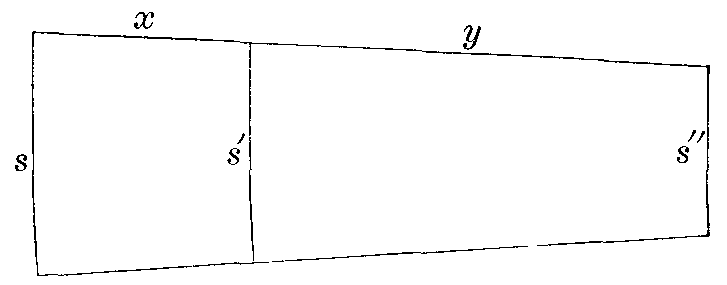
\includegraphics[width=70mm]{fig47.png}
\end{figure}

同じ軸の組をもつ三つの限界曲線から、
\begin{equation*}
f(x+y) = f(x)f(y)
\end{equation*}
を得る。この性質は指数関数に特有のもので、その一般形は $f(x)= e^{ax}$ である。\footnote{$y = x$、$2x$、$\cdots$ $(n-1)x$ を順次代入すると、$x$ を任意の正の量として、正の整数値 $n$ に対して
\begin{equation*}
f(nx) = [f(x)]^n
\end{equation*}
を得る。
\par ところで、
\begin{equation*}
f\left(\frac{r}{s}x\right) = \left[f\left(\frac{x}{s}\right)\right]^r
\end{equation*}
であり、これは等式
\begin{equation*}
\left[f\left(\frac{x}{s}\right)\right]^s = f(x)
\end{equation*}
の左辺の $s$ 乗根の $r$ 乗である。したがって、
\begin{equation*}
f\left(\frac{r}{s}x\right) = [f(x)]^\frac{r}{s}.
\end{equation*}
こうして、$f(x)$ が $x$ の連続関数であると仮定すれば、$x$ と $n$ のすべての実数の正の値に対して
\begin{gather*}
f(nx) = [f(x)]^n, \\
\intertext{が証明され、$n$ に $x$ を、$x$ に $1$ を代入すれば、}
f(x) = [f(1)]^x
\end{gather*}
を得る。
\par $f(1) = e^a$ と書くと、
\begin{equation*}
f(x) = e^{ax}
\end{equation*}
となる。} したがって、$\dfrac{s}{s'}= e^{ax}$ であり、$a$ の値は測定の単位に依存する（後述の該当ページを見よ）。

\item[3.~定理.] \emph{同じ軸をもつ二つの限界曲線と、それらの共通な二つの軸とで囲まれた面積は、切り取られた弧の差に比例する。}

\begin{figure}[h]
\centering
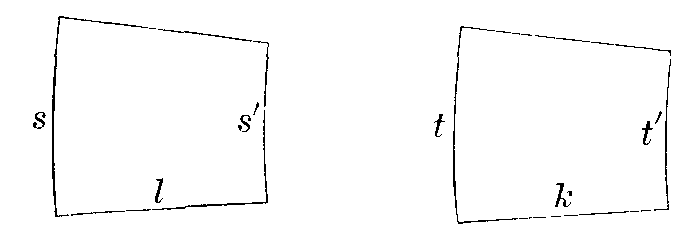
\includegraphics[width=60mm]{fig48.png}
\end{figure}

\textbf{証明.} $s$ と $s'$ を切り取られた弧の長さ、$l$ を軸上で測った、それらの間の距離とする。同様にしてつくった第二の図形について、対応する量を $t$、$t'$、$k$ とする。

二つの図形の対応する線がすべて等しければ、重ね合わせることができるから、面積は等しい。$k = l$ だけが成り立つならば、面積は対応する弧、たとえば $s' : t'$ の比になる。これは、まず弧が通約できる場合に証明し、ついで通約できない場合には極限の方法によって証明する。

\begin{figure}[h]
\centering
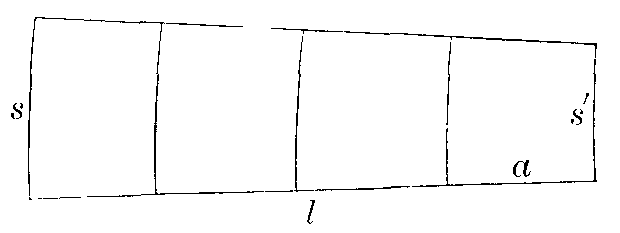
\includegraphics[width=60mm]{fig49.png}
\end{figure}

$l$ と $k$ が通約できるとき、
\begin{equation*}
\frac{l}{m} = \frac{k}{n} = a
\end{equation*}
とする。軸上に、$a$ に等しい距離ごとに一連の限界曲線を引き、面積をそれぞれ $m$ 個と $n$ 個の部分に分けることができる。距離 $a$ に対応する弧の比を $r$ とすれば、これらの部分は、次の量に比例する。
\begin{gather*}
  s',\ s'r,\ s'r^2,\dots s'r^{m-1};\\
  t',\ t'r,\ t'r^2,\dots t'r^{n-1}.
\end{gather*}

したがって二つの面積の比は、
\begin{equation*}
  s' \frac{r^m-1}{r-1} \colon t' \frac{r^n-1}{r-1}
\end{equation*}
である。

しかるに、
\begin{equation*}
  s'r^m = s \text{ かつ } t'r^n = t
\end{equation*}
であるから、これは比
\begin{equation*}
  s-s' \colon t-t'
\end{equation*}
と同じである。

$l$ と $k$ が通約できないときは、他の同様な証明のように進める。

この定理は、多角形について証明した定理と類似している。すなわち、面積は、図形を一周するときの、四直角を超える回転量に比例し、限界曲線に沿って進むときの回転の割合は一定だからである。

\begin{figure}[h]
\centering
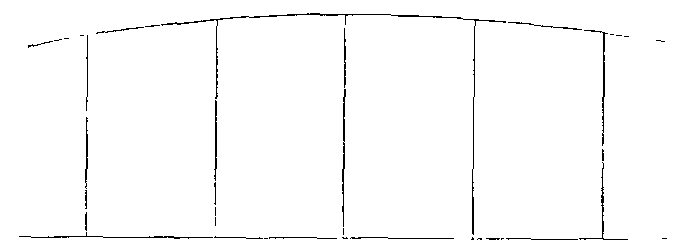
\includegraphics[width=60mm]{fig50.png}
\end{figure}

直線から与えられた距離にある点の軌跡は、\emph{等距離曲線}と呼ぶことのできる曲線である。この曲線の異なる点から基線へ下ろした垂線は等しく、曲線の\emph{軸}と呼ぶことができる。

等距離曲線は、その軸の一つのまわりに二直角だけ回転させたとき、あるいはそれ自身の上を滑らせたとき、それ自身に重なる。曲率は一定である。

同じ軸の組をもつ二つの限界曲線の場合とまったく同様に、等距離曲線上の弧は、その軸が基線上に、あるいは同じ軸の組をもつ他の任意の等距離曲線上に、端点で切り取る線分に比例することを証明できる。


\item[4.~定理.] \emph{限界曲線は、円と等距離曲線との間の極限の曲線である。それは半径が無限に大きい円とも、基線が無限に遠い等距離曲線ともみなせる。}

\begin{figure}[h]
\centering
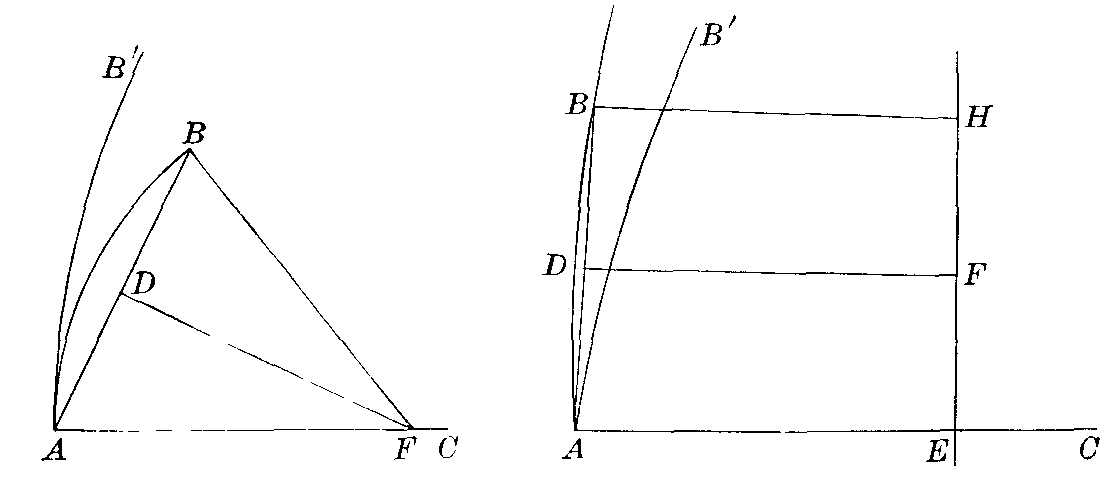
\includegraphics[width=80mm]{fig51.png}
\end{figure}

\textbf{証明.} 与えられた長さの線 $AB = 2a$ をとり、固定した線 $AC$ と角 $A$ をなすものとする。$B$ に角 $A$ に等しい別の角をつくり、$AB$ の中点 $D$ で $AB$ に垂線を引く。

$A$ での角が十分に小さければ、$AB$ を底辺とし、頂点が $AC$ 上の点 $F$ にある二等辺三角形ができる。$F$ を中心として、点 $A$ と $B$ を通る円を描くことができる。そこで $A$ での角を徐々に増し、図の他の部分は作図を保つように変化させる。$F$ は限りなく遠ざかり、$A = \Pi(a)$ となったとき、三本の線 $AF$、$BF$、$DF$ は平行になり、$B$ は、$AC$ を軸とする限界曲線 $AB'$ 上の点になる。

一方、$A$ での角を鋭角にとるが $\Pi(a)$ より大きくとれば、点 $A$ と $B$ を通る等距離曲線の基線 $EH$ に垂直な三本の線 $AE$、$BH$、$DF$ ができる。そこで角 $A$ を徐々に減らし、図の他の部分は作図を保つように変化させる。三つの直角をもち、第四の角 $A$ が減少する四角形 $ADFE$ は、面積が増加しなければならない。これと同じ動きは、$AD$ と $DF$ が平面上で固定されたまま、$AE$ が $A$ のまわりに回転して角 $A$ が減少すると考えても得られる。このように、四角形の面積が増加しうる唯一の方法は、$EH$ が $AC$ に沿って遠ざかり、$A$ からますます遠くなることである。$A$ が $\Pi (a)$ に等しくなるとき、$BH$ と $DF$ は $AC$ に平行になり、$B$ は限界曲線 $AB'$ の上に落ちる。
\end{description}

円の半径を軸と呼ぶことにすると、円、限界曲線、等距離曲線には共通の性質が多いことがわかる。

任意の弦の中点に立てた垂線は軸である。とくに、接線は、その接点から引いた軸に垂直である。これらは、それぞれ、一点を通る線の系、平行線の系、与えられた線への垂線の系を直角に切る曲線である。

同じ軸の組をもつこれらの曲線の二つは、これらの軸のすべてに等しい長さを切り取り、そのような二つの曲線上の対応する弧の比は、軸の分け方だけに依存する定数である。

三点がこれらの曲線の一つを定める。すなわち、一直線上にない任意の三点を通って、円か、限界曲線か、等距離曲線のいずれかである曲線を引くことができ、任意の三点を通る曲線はただ一つしか引けない。任意の三角形は、これらの曲線のただ一つに内接させることができる。

これらの曲線の各々は、それ自身の上を動かすことができ、また任意の軸のまわりに $180^\circ$ 回転させてそれ自身に重ねることができる。

\emph{限界面}あるいはオリスフィアとは、限界曲線をその軸の一つのまわりに回転させて生じる曲面である。

\begin{description}
\item[5.~定理.] \emph{限界面の軸に平行な任意の線を軸とみなすことができる。}

\begin{figure}[h]
\centering
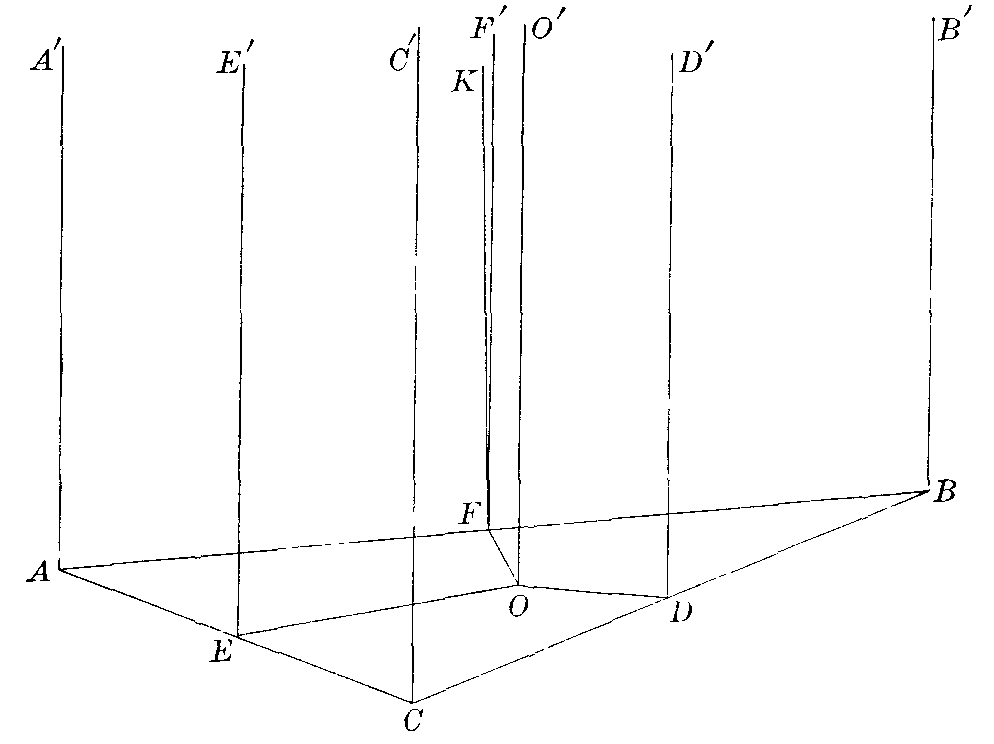
\includegraphics[width=80mm]{fig52.png}
\end{figure}

\textbf{$AA'$} を、曲面と $A$ で出会う軸とし、$BB'$ を曲面の任意の他の点 $B$ を通る軸に平行な線とする。$BB'$ を軸とみなせることを証明する。

\textbf{証明.} $C$ を曲面上の第三の点とする。$C$ を通って $CC'$ を引き、平面三角形 $ABC$ の各辺の中点 $D$、$E$、$F$ を通って、すべて $AA'$ に平行な $DD'$、$EE'$、$FF'$ を引く。最後に、これらの線に平行で平面 $ABC$ に垂直な $OO'$ を引く。他の平行線の射影平面は、すべて $OO'$ を通る（I, 9 を見よ）。

$AA'$ は曲面の軸であるから、$EE'$ と $FF'$ は、それぞれ $AC$ と $AB$ に垂直である。$F$ で平面 $ABC$ に垂直に $FK$ を引く。それは射影平面 $OFF'$ に含まれる。$AB$ は $FF'$ と $FK$ に垂直であるから、この平面 $OFF'$ に、したがって $OF$ に垂直である。同様にして、$AC$ が $OE$ に垂直であることが証明される。したがって、$BC$ は $OD$ に垂直である（第I章, I, 5）。しかるに $OD$ は平面 $ABC$ と平面 $ODD'$ の交線である。ゆえに $BC$ はこの平面に、また $DD'$ に垂直である（第I章, II, 15）。

$DD'$ は $BB'$ に平行であるから、$BB'$ と $BC$ で定まる平面に含まれ、この平面内では、$BC$ にその中点で垂直な線はただ一本しか引けない。したがって、$BB'$ を通る任意の平面をとり、$B$ からこの平面と曲面との交わりの任意の他の点 $C$ へ弦を引くと、この平面内で $BC$ の中点に立てた $BC$ への垂線は $BB'$ に平行である。これは、断面が $BB'$ を軸とする限界曲線であり、曲面がそのような限界曲線を $BB'$ のまわりに回転させて生成できることを証明している。

ゆえに、$BB'$ は曲面の軸とみなせる。
\end{description}

限界面の軸を通る平面を\emph{主平面}という。すべての主平面は、曲面を限界曲線で切る。他の任意の平面は、曲面を円で切る。なぜなら、曲面は、その平面に垂直な軸を回転軸とする回転面とみなせるからである。この垂線を円の軸と呼び、それが曲面と出会う点を円の\emph{極}と呼ぶことができる。限界面上の円の極は、円のすべての点から等しい距離にある。ここで距離は、曲面上の限界線に沿って測る。

任意の二つの限界面を重ね合わせることができ、限界面は、任意の点を任意の他の点の位置へ、また最初の点を通る任意の限界曲線を第二の点を通る任意の限界曲線の位置へ、それ自身の上で動かすことができる。限界面は一定の曲率をもち、それはすべてのこれらの曲面で同じであると言ってよい。限界面上の図形は、形も大きさも変えずに動かすことができ、他の任意の限界面の上に置くことができる。

限界面上に幾何学を展開することができる。\emph{線}とは、曲面を主平面で切ってできる限界曲線を指す。二つの線のなす角は、曲面上にその線を切り出す二つの主平面の二面角に等しい。

\begin{description}
\item[6.~定理.] \emph{限界面上の幾何学は、通常のユークリッドの平面幾何学と同じである。}

\textbf{証明.} 同じ平行線の系を軸とする二つの限界面上では、対応する三角形は相似である。すなわち、対応する角は、それらを切り出す二面角と同じ大きさで等しく、対応する線は (2) により比例する。しかしこれらの図形を同じ曲面の上に置くことができるから、一つの限界面上に相似な三角形をもてる。こうして、三角形の辺を、その比も角も変えずに小さくできる。これは限りなく行える。なぜなら、二つの曲面上の対応する線の比は、それらの間の距離の関数 $e^{ax}$ で表されるから、$x$ を十分大きくとることにより望むだけ大きくできるからである。限界面上の図形は、その大きさを限りなく小さくするにつれて、ますます平面図形に似てゆくと仮定すれば、この曲面上の三角形は、角の和が二直角で、角と辺の関係がユークリッドの平面幾何学と同じである無限小の平面三角形の形に、ますます近づいてゆくことになる。したがって、われわれになじみのある平面三角法の公式はすべて、限界面上の三角形について成り立つ。

限界面上では「直角の仮説」が成り立つ。長方形をつくることができ、長方形の面積は底辺と高さの積に比例し、三角形の面積は、同じ底辺と高さをもつ長方形の面積の半分である。
\end{description}

\emph{等距離面}とは、等距離曲線をその軸の一つのまわりに回転させて生じる曲面である。それは、平面から与えられた垂直距離にある点の軌跡である。平面への任意の垂線を軸とみなすことができ、この曲面は、平面に垂直な線の系を直角に切る曲面である。この曲面は一定の曲率をもち、任意の位置でそれ自身に重なる。

\section{三角法の公式}

\begin{description}
\item[1.~] $ABC$ を平面の直角三角形とする。その平面に垂直に $AA'$ を立て、$AA'$ に平行に $BB'$ と $CC'$ を引く。$A$ を通り、これらの線を軸とする限界面を描き、限界面上の三角形 $AB''C''$ をつくる。また、点 $B$ のまわりに球面三角形をつくる。

\begin{figure}[h]
\centering
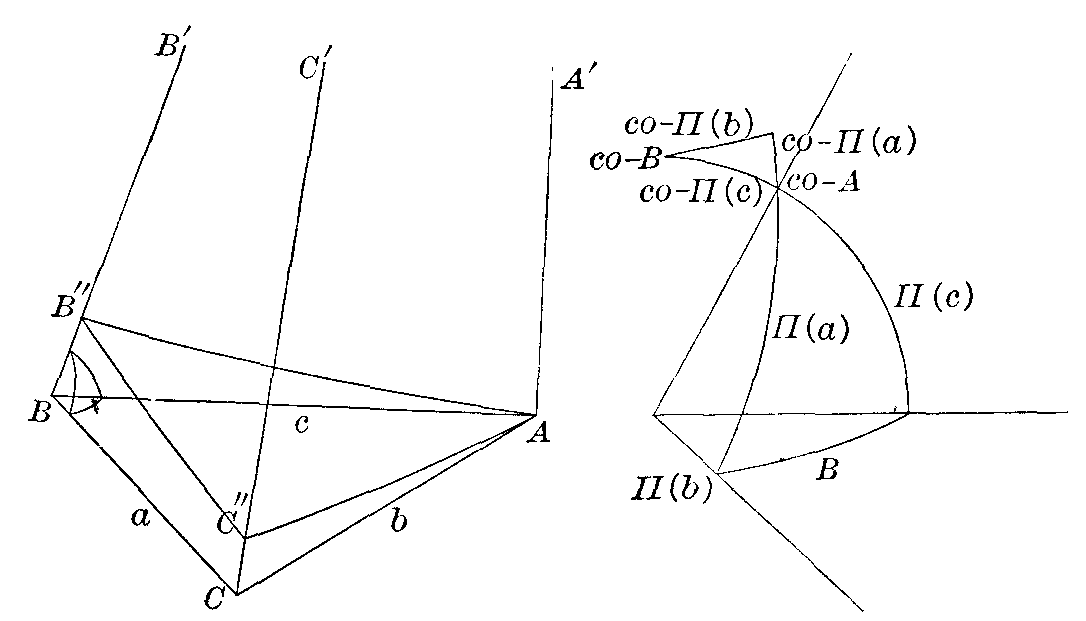
\includegraphics[width=80mm]{fig53.png}
\end{figure}

角 $A$ は、平面三角形と限界面上の三角形とで同じである。$AA'$ を通る平面は $ABC$ に垂直である。したがって、球面三角形は $c$ 上にある頂点に直角をもち、$CA$ に垂直な $BC$ は、$CC'$ と $AA'$ の平面に垂直である。ゆえに、平面 $BCC'$ は平面 $ACC'$ に垂直であり、辺が $BC$ である二面角の平面角は、角 $ACC'= \Pi (b)$ である。限界面上の三角形は $C''$ に直角をもつから、角 $B''$、あるいは同じことだが、辺が $BB'$ である二面角は、角 $A$ の余角である。

球面三角形では、直角に対する辺は $\Pi (a)$、直角をはさむ二辺は $\Pi (c)$ と $B$ であり、対する角は $\Pi (b)$ と $90^\circ-A$ である。

これらの量に球面直角三角形の三角法の公式を適用すると、ただちに平面直角三角形の辺と角を結ぶ関係が得られる。

$A$ の余角に等しい値をもつ角をはさむ二辺を、象限まで延長する。このようにして、直角に対する辺が $\Pi(c)$ の余角であり、直角をはさむ二辺が $\Pi(a)$ と $\Pi (b)$ の余角であり、それらに対する角が $B$ と $A$ の余角である球面直角三角形ができる。この三角形から、球面直角三角形の公式から平面三角形の公式へ移るための次の規則を導く。

\emph{二つの角（または二つの辺）を入れ替え、至るところで余関数を用い、辺については対応する平行角をとる。}

球面直角三角形の公式は、次のとおりである。
\begin{gather*}
\begin{aligned}
\sin A &= \frac{\sin a}{\sin c}. & \sin B &= \frac{\sin b}{\sin c}.\\
\cos A &= \frac{\tan b}{\tan c}. & \cos B &= \frac{\tan a}{\tan c}.\\
\tan A &= \frac{\tan a}{\sin b}. & \tan B &= \frac{\tan b}{\sin a}.\\
\sin A &= \frac{\cos B}{\cos b}. & \sin B &= \frac{\cos A}{\cos a}.
\end{aligned}\\
\begin{aligned}
\cos c &= \cos a \cdot \cos b \\
\cos c &= \cot A \cdot \cot B \\
\end{aligned}
\end{gather*}

これらから、前に与えた規則によって、平面直角三角形の次の公式を導く。
\begin{gather*}
  \begin{aligned}
    \cos B &= \frac{\cos\Pi(a)}{\cos\Pi(c)}. &
    \cos A &= \frac{\cos\Pi(b)}{\cos\Pi(c)}.\\
    \sin B &= \frac{\cot\Pi(b)}{\cot\Pi(c)}. &
    \sin A &= \frac{\cot\Pi(a)}{\cot\Pi(c)}.\\
    \cot B &= \frac{\cot\Pi(a)}{\cos\Pi(b)}. &
    \cot A &= \frac{\cot\Pi(b)}{\cos\Pi(a)}.\\
    \cos B &= \frac{\sin A}{\sin\Pi(b)}. &
    \cos A &= \frac{\sin B}{\sin\Pi(a)}.
  \end{aligned}\\
  \begin{aligned}
    \sin\Pi(c) &= \sin\Pi(a) \sin\Pi(b).\\
    \sin\Pi(c) &= \tan A \tan B.\footnotemark
  \end{aligned}
\end{gather*}
\footnotetext{直角三角形の各部分を、ネイピアの規則を適用できるように並べることができる。すなわち、配置は次のようになる。

\centering
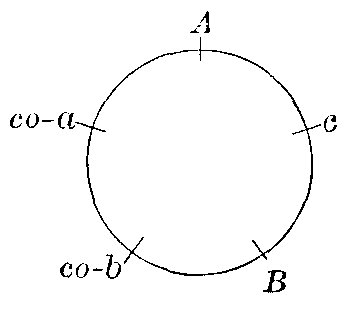
\includegraphics[width=30mm]{fig54.png}}

斜角の平面三角形の公式は、一つの頂点から対辺へ垂線を下ろし、二つの直角三角形をつくることによって得られる。

\item[2.~] 関係
\begin{equation*}
  \sin\Pi(a) = \frac{\sin B}{\cos A}
\end{equation*}
をとる。

\textbf{$p$}、$q$、$r$ を、前の証明の三角形 $AB''C''$ の辺とし、$p'$、$q'$、$r$ を、$B$ で平面 $ABC$ に接する限界面上に同じ方法でつくった三角形の対応する辺とする。

\begin{figure}[h]
\centering
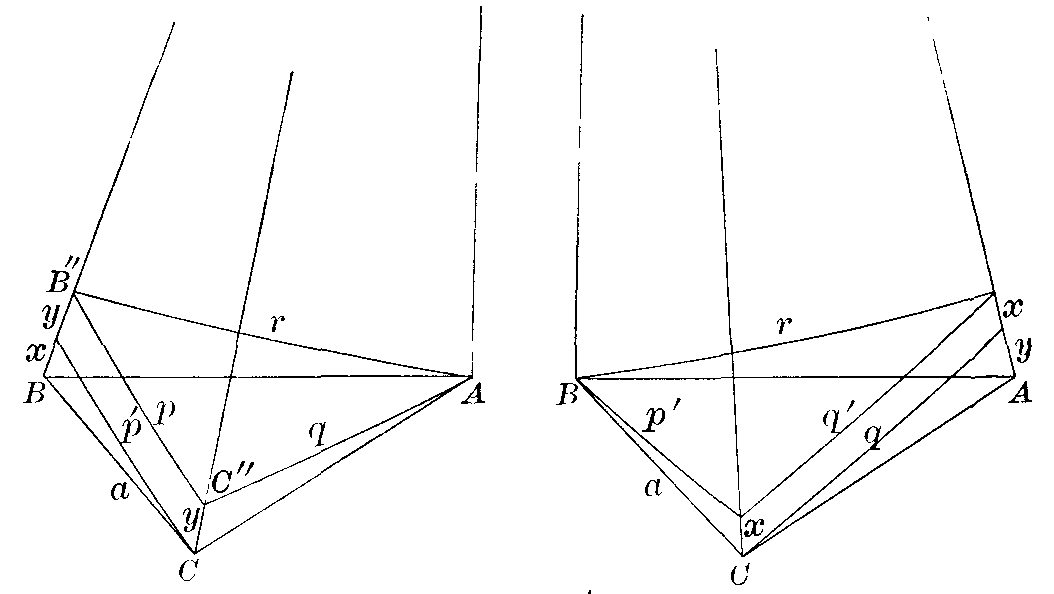
\includegraphics[width=80mm]{fig55.png}
\end{figure}

\begin{align*}
  \sin B &= \frac{q'}{r}, \\
  \cos A &= \frac{q}{r} . \\
  \therefore \sin \Pi(a) &= \frac{q'}{q} .
\end{align*}

\begin{figure}[h]
\centering
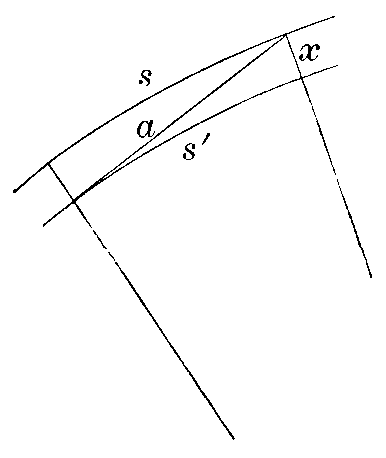
\includegraphics[width=35mm]{fig56.png}
\end{figure}

ここで $q$ と $q'$ は、同じ平行線の組を軸とする二つの限界曲線上の対応する弧であり、それらの間の距離 $x$ は、任意の長さ $a$ の接線の端点から限界曲線までの距離である。したがって、対応する弧について、
\begin{equation*}
  \frac{s'}{s} = \sin \Pi(a)
\end{equation*}
が成り立つ。


\begin{figure}[h]
\centering
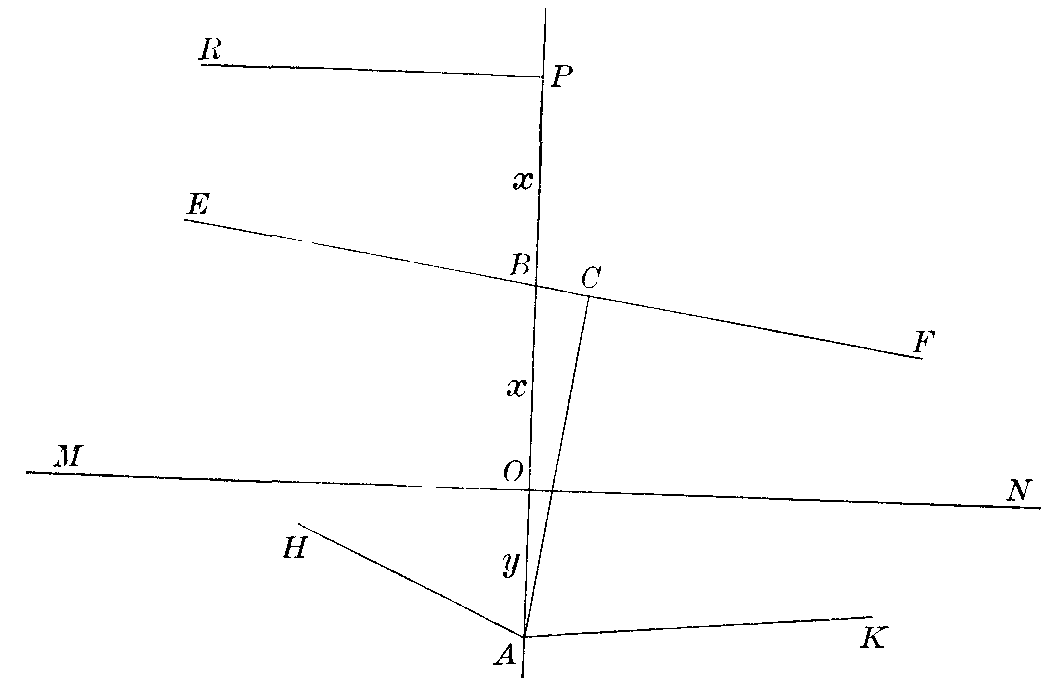
\includegraphics[width=80mm]{fig57.png}
\end{figure}

\item[3.~] 与えられた直線 $MN$ の点 $O$ に垂線を立て、この垂線上に、$MN$ の下側に $OA = y$ をとり、$MN$ の上側に $OB$ と $BP$ をそれぞれ $x$ にとる。$x$ と $y$ は任意の長さとする。$P$ で $OP$ に垂直に、左へ延びる $PR$ を引き、$B$ を通って、$OP$ と角 $\Pi (x)$ をなす $EF$ を引く。これは一方では $ON$ に、他方では $PR$ に平行である。最後に、$A$ を通る $EF$ への二本の平行線 $AK$ と $AH$ を引く。

点 $A$ には四つの平行角がある。
\begin{align*}
 CAK = CAH &= \Pi (AC),       \\
       OAK &= \Pi (y) ,       \\
       PAH &= \Pi (y+2x) .    \\
\intertext{したがって、}
   \Pi (y) &= \Pi (AC) + BAC ,\\
\intertext{および}
\Pi (y+2x) &= \Pi (AC) - BAC . \\
\intertext{さて直角三角形 $ABC$ において}
\cos \Pi (y + x) &= \frac{\cos \Pi (AC)}{\cos BAC} \\
\intertext{すなわち}
  \frac{1-\cos \Pi (y+x)}{1+\cos \Pi (y+x)}
&= \frac{\cos BAC - \cos \Pi (AC)}{\cos BAC + \cos \Pi (AC)}, \\
&= \frac{ \sin \tfrac{1}{2} \left[ \Pi (AC) + BAC \right]
          \sin \tfrac{1}{2} \left[ \Pi (AC) - BAC \right] }
        { \cos \tfrac{1}{2} \left[ \Pi (AC) + BAC \right]
          \cos \tfrac{1}{2} \left[ \Pi (AC) - BAC \right] }; \\
\intertext{ゆえに、}
\tan^2 \tfrac{1}{2} \Pi (y + x)
  &= \tan \tfrac{1}{2} \Pi (y) \tan \tfrac{1}{2} \Pi (y + 2x)
\end{align*}

そこで $\tan \frac{1}{2} \Pi(x)$ は $x$ の関数、たとえば $f(x)$ であって、条件
\begin{align*}
  \left[ f(y + x) \right]^2 & = f(y) f(y+2x) \\
\intertext{すなわち}
  \frac{f(y+x)}{f(y)} & = \frac{f(y+2x)}{f(y+x)}
\end{align*}
を満たす。この式の $y$ に $y + x$、$y + 2x$、$\cdots$ を順次代入してゆくと、さらに
\begin{equation*}
= \frac{f(y+3x)}{f(y+2x)} = \cdots
= \frac{f(y+nx)}{f \left[ y+(n-1)x \right]}
\end{equation*}
を加えることができる。

$\Pi (0) = \frac{\pi}{2}$ で $\tan \tfrac{1}{2} \Pi (0) = 1$ であるから、これらすべての分数の最初と最後に $y = 0$ を代入すると、
\begin{align*}
  f(x) & = \frac{f(nx)}{f\left[ (n-1) x\right]} , \\
\intertext{すなわち}
  f(nx) & = f\left[(n-1)x \right] f(x). \\
\therefore f(nx) & = \left[ f(x)\right]^n
\end{align*}
を得る。

この式は指数関数に特有のものである。\footnote{前出の脚注を見よ。} $\Pi (x)$ は鋭角であるから $\tan \tfrac{1}{2} \Pi (x) < 1$ であり、したがって $f(1) = e^{-a'}$ と書けて、$f(x) = e^{-a'x}$ となる。$a'$ は測定の単位に依存する。ここでは $a' = 1$ となるように単位をとる。最後に、$\Pi(-x) = \pi - \Pi (x)$ であるから、
\begin{equation*}
\tan \tfrac{1}{2} \Pi (-x)
  = \cot \tfrac{1}{2} \Pi (x)
  = \left[ \tan \tfrac{1}{2} \Pi (x) \right]^{-1}
\end{equation*}
である。
\newpage
すなわち、$x$ のすべての実数値に対して、
\begin{align*}
    \tan \tfrac{1}{2} \Pi (x) &= e^{-x} ,
\intertext{すなわち}
\frac{1-\cos\Pi(x)}{\sin\Pi(x)}
  &= \cos ix + i\sin ix.\footnotemark
\end{align*}
\footnotetext{$i$ は $\sqrt{-1}$ を表す。指数関数と三角関数の関係を得る最良の方法は、それらの級数展開によるものである。
\begin{align*}
  e^x &= 1 + x + \frac{x^2}{2!} + \dots + \frac{x^n}{n!} + \dotsb,\\
  \cos x &= 1 - \frac{x^2}{2!} + \frac{x^4}{4!} - \dots +
           (-1)^n\frac{x^{2n}}{2n!} + \dotsb,\\
  \sin x &= x - \frac{x^3}{3!} + \frac{x^5}{5!} - \dots +
           (-1)^n\frac{x^{2n+1}}{(2n+1)!} + \dotsb.
\end{align*}
\par これらの級数は $x$ のすべての値に対して収束する。
\par $x$ に $ix$ を代入すると、
\begin{gather*}
  \begin{aligned}
    e^{ix} &= 1 + ix - \frac{x^2}{2!} - \frac{ix^3}{3!} + \dotsb\\
    &= 1 - \frac{x^2}{2!} + \frac{x^4}{4!} - \dots +
    i\left( x - \frac{x^3}{3!} + \frac{x^5}{5!} - \dotsb \right);
  \end{aligned} \\
  \begin{aligned}
\text{すなわち}\qquad e^{ix}  &= \cos x + i\sin x.\\
\text{また}\qquad e^{-ix} &= \cos x - i\sin x.\\
    \therefore \cos x &= \tfrac{1}{2} \left(e^{ix} + e^{-ix}\right),\\
    \sin x &= \tfrac{1}{2i} \left(e^{ix} - e^{-ix}\right).
  \end{aligned}
\end{gather*}
\par さらに、$x$ に $ix$ を代入すると、
\begin{align*}
  e^x &= \cos ix - i\sin ix,\\
  e^{-x} &= \cos ix + i\sin ix;\\
  \intertext{および}
  \cos ix &= \tfrac{1}{2} \left(e^x + e^{-x}\right),\\
  \sin ix &= -\tfrac{1}{2i} \left(e^x - e^{-x}\right).\\
  \cos ix &= 1 + \frac{x^2}{2!} + \frac{x^4}{4!} + \dotsb,\\
  \sin ix &= ix \left(1 + \frac{x^2}{3!} + \frac{x^4}{5!}
                                                     + \dotsb\right).
\end{align*}
\par $x$ の実数値に対して、$\cos ix$ と $\dfrac{\sin ix}{ix}$ は実数で正であり、$x$ が $0$ から $\infty$ まで変化するとき、$1$ から $\infty$ まで変化する。
\par 等式 $\cos^2ix + \sin^2ix = 1$ において、第一項は $x$ の実数値に対して実数で正であり、第二項は実数で負である。したがって、$\sin ix$ は絶対値において $\cos ix$ より小さく、$\tan ix$ は絶対値において $1$ より小さい。$\tan ix$ は、$x$ が $0$ から $\infty$ まで変化するとき、絶対値において $0$ から $1$ まで変化する。}

$x$ の符号を変えると、
\begin{align*}
\frac{1+\cos\Pi(x)}{\sin\Pi(x)} &= \cos ix - i \sin ix, \\
\intertext{加えたり引いたりして、}
\frac{1}{\sin\Pi(x)} &= \cos ix, \\
\cot\Pi(x) &= -i\sin ix
\end{align*}
を得る。

したがって、平行角の性質は、方程式
\begin{align*}
\sin\Pi(x) &= \frac{1}{\cos ix}, \\
\tan\Pi(x) &= \frac{i}{\sin ix}, \\
\cos\Pi(x) &= \frac{\tan ix}{i}
\end{align*}
で表される。

\item[4.~] 平面直角三角形の公式に代入すると、それらは、$a$、$b$、$c$ の代わりにそれぞれ $ia$、$ib$、$ic$ を用いた球面直角三角形の公式に帰着することがわかる。斜角三角形の公式は、球面上と同じ方法で直角三角形の公式から得られ、こうして、平面三角法のすべての公式が、球面三角法の公式からこの変更をするだけで得られる。

斜角三角形の基本公式として、次を書く。
\begin{gather*}
\frac{\sin A}{\sin ia} = \frac{\sin B}{\sin ib}
                       = \frac{\sin C}{\sin ic}, \\
\cos ia = \cos ib\, \cos ic + \sin ib\, \sin ic\, \cos A, \\
\cos A  = -\cos B\, \cos C + \sin B\, \sin C\, \cos ia.
\end{gather*}

$\Pi$ 関数の記法では、これらは次のようになる。
\begin{gather*}
\sin A\, \tan\Pi(a) = \sin B\, \tan\Pi(b) = \sin C\, \tan\Pi(c), \\
\frac{\sin\Pi(b)\,\sin\Pi(c)}{\sin\Pi(a)} =
                             1-\cos\Pi(b)\,\cos\Pi(c)\,\cos A, \\
\cos A = -\cos B\, \cos C + \frac{\sin B\,\sin C}{\sin\Pi(a)}.
\end{gather*}

\item[5.~] $x$ が非常に小さい値のとき、近似的に
\begin{gather*}
\sin ix = ix, \\
\cos ix = 1 + \frac{x^2}{2}, \\
\tan ix = ix, \\
\intertext{であるから、無限小の三角形についての公式は次に帰着する。}
\frac{\sin A}{a} = \frac{\sin B}{b} = \frac{\sin C}{c}, \\
a^2 = b^2 + c^2 - 2bc\,\cos A, \\
\cos A = -\cos(B+C).
\end{gather*}

\item[6.~] 等距離面上の三角形は、基底平面への射影と相似である。すなわち、角が同じで、辺が比例する。したがって、平面三角法の公式は、辺を表す文字に、$i$ のほかに、曲面の平面からの距離に依存する定数因子をつければ、任意の等距離面について成り立つ。
\end{description}


\chapter{楕円幾何学（リーマン幾何学）}

鈍角仮説においては、直線は有限の長さを持ち、自身へと戻る閉じた線となる。任意の2直線は合同変換によって重ね合わせることができるため、すべての直線はまったく同一の有限の長さを持つ。2直線は常に必ず交わり、同一の直線に対して垂直な2本の直線は、その直線から測って「直線の全長の半分」の距離にある点において互いに交差する。

\begin{figure}[htbp]
\centering
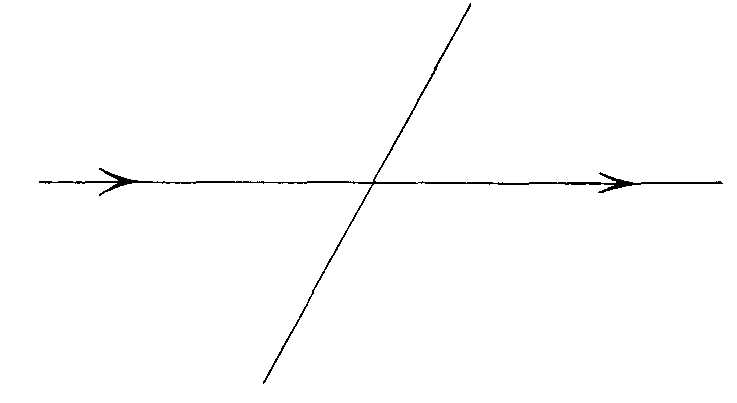
\includegraphics[width=70mm]{fig58.png}
\caption{楕円平面における直線と極・極線の構造}
\end{figure}

\begin{enumerate}[label=\textbf{\arabic*.}]
\item \textbf{直線は平面を2つに分割しない}：
2直線の交点を出発し、一方の直線に沿ってある有限の距離を進むと、他方の直線を一度も横切ることなく再び元の交点へと戻ってくることができる。すなわち、直線を横断することなく、その直線の「一方の側」から「他方の側」へと移動することが可能である（メビウスの帯・射影平面のトポロジー）。

与えられた直線に対するすべての垂線はある1点で交わる。この点をその直線の\textbf{極（pole）}と呼び、直線はその極の\textbf{極線（polar）}と呼ばれる。極から極線までの距離は「直線の全長の半分」であり、極線は極からこの等距離にある点の軌跡である。したがって、ある直線の極が別の直線の上にあれば、第2の直線の極は第1の直線の上にあり、2直線の交点は、両者の極を結ぶ直線の極となる。

与えられた直線から一定の距離にある点の軌跡は、その直線の極を中心とする円となる。直線とは、半径が直線の全長の半分に達したときの円の極限形式に他ならない。

互いに直交する3本の直線を描くことができ、これによって\textbf{3直角三角形（三直角三角形）}が形成される。この三角形は\textbf{自己極三角形（self-polar triangle）}でもあり、各頂点は対辺の極となっている。

\item \textbf{空間における極と平面}：
空間内において、ある平面に対するすべての法線は1点で交わり、この点がその平面の\textbf{極}となる。極は、半径が直線の全長の半分に達したときに平面を極限形として含む球面系の中心である。

平面上の図形は、平面の極を中心とする任意の球面上にある相似な図形から射影することができる。すなわち、対応する角は等しく、対応する辺の長さは球の半径のみに依存する一定の比率を持つ。

したがって、楕円平面上の幾何学は球面幾何学に酷似しているが、楕円平面は球面全体の「半分」（対蹠点を同一視した半球）に対応する。球面の中心を通る直径が球面の半分の点に対応するのと同様である。半球の境界にある直径の両端点が互いに同一である（貼り合わされている）と想像すれば、その半球は楕円平面と厳密に対応する。楕円平面には境界となる特定の直線は存在せず、すべての直線は対等である。平面は有界（限界）を持たないが、有限の広がり（面積）しか持たない。

直線の全長を $\pi$ とするような長さの単位系を選ぶと、球面三角法の公式が一切の変更なしにそのまま楕円平面に適用できる。直線上の距離は、その直線が極において張る中心角と同一の尺度を持ち、2直線のなす角はそれらの極の間の距離に等しくなる。任意の点からその極線までの距離（直線の全長の半分）は、これを\textbf{象限（quadrant, $\pi/2$）}と呼ぶことができる。

互いに直交する3つの平面と、それらの交点を極とする平面をとることにより、\textbf{自己極四面体}を作ることができる。この四面体の各頂点は対面の極であり、各頂点には3直角の三面角が存在し、各面は3直角三角形である。
\end{enumerate}

\begin{tcolorbox}[colback=white,colframe=blue!75!black,title=\textbf{定理 3}]
\emph{一定の直線に垂直なすべての平面は、別の固定された直線において交わる。この直線をもとの直線の\textbf{極線（共役線：conjugate）}と呼ぶ。この関係は相互的（相反的）であり、一方の直線上のすべての点は、他方の直線上のすべての点からちょうど象限（$\pi/2$）の距離にある。}
\end{tcolorbox}

\begin{figure}[htbp]
\centering
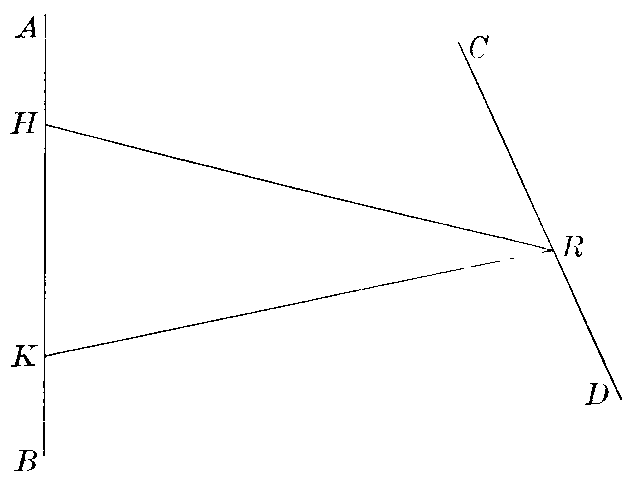
\includegraphics[width=60mm]{fig59.png}
\caption{共役直線と極線の相互関係}
\end{figure}

\textbf{【証明】}
直線 $AB$ に点 $H, K$ で垂直な2つの平面が直線 $CD$ で交わるとする。$AB$ および $CD$ 上の任意の点 $R$ を通る平面を考える。この平面は与えられた2つの平面とそれぞれ $HR$ および $KR$ で交わる。$HR, KR$ はともに $AB$ に垂直であるから、点 $R$ は点 $H, K$ の双方から象限の距離にある。したがって $R$ は、線分 $AR$ と点 $R$ で定まる平面において $AB$ の極であり、$AB$ 上のすべての点から象限の距離にある。
しかし $R$ は $CD$ 上の任意の点であったから、いずれの直線上の任意の点も、他方の直線上の各点から象限の距離にある。自己極四面体の対向する辺は互いに極線（共役線）の関係にある。

与えられた直線と直角に交わるすべての直線は、その共役線とも直角に交わる。したがって、任意の点から2つの共役線への距離は同一の直線上で測られ、その和は常に1象限（$\pi/2$）に等しい。ある直線から等距離にある2点は、その共役線からも等距離にある。

固定された直線から一定の距離にある点の軌跡は、その直線とその共役線の双方を回転軸とする回転面となる。これを\textbf{二重回転面（surface of double revolution）}と呼ぶ。一方の軸に関する緯線円は、他方の軸に関する子午線曲線となる。空間全体がある直線に沿ってその周りの回転を伴わずに移動するとき、空間はその共役線を軸として滑りを伴わずに回転する。直線に沿った平行移動と直線の周りの回転を組み合わせた運動を\textbf{ねじれ運動（screw motion）}と呼ぶ。したがって、ねじれ運動は2つの共役線のそれぞれに関する回転、または2つの共役線のそれぞれに沿った平行移動として記述できる。

\begin{tcolorbox}[colback=white,colframe=blue!75!black,title=\textbf{定理 4（クリフォードの平行線）}]
\emph{楕円幾何学においては、同一平面上にない直線でありながら、無数の共通垂線を持ち、至る所等距離であるような直線の対が存在する。}
\end{tcolorbox}

\begin{figure}[htbp]
\centering
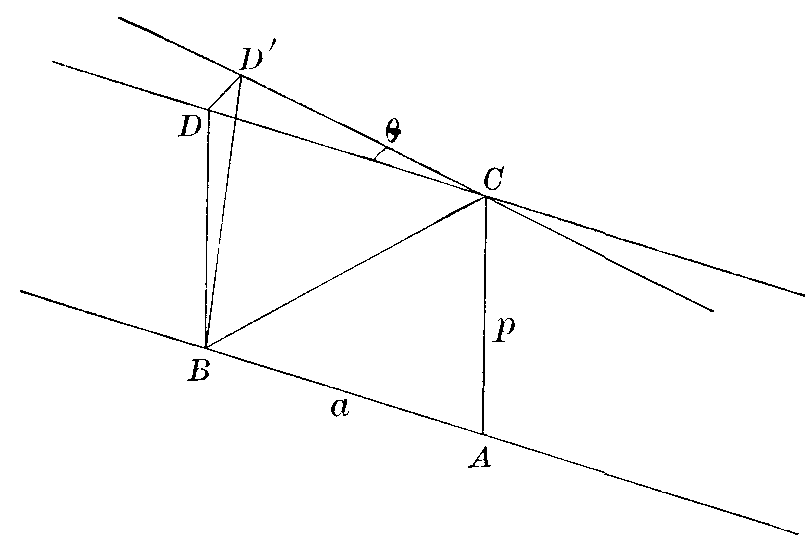
\includegraphics[width=80mm]{fig60.png}
\caption{クリフォードの平行線（至る所等距離な非共面直線）}
\end{figure}

\textbf{【証明】}
同一平面上にある任意の2直線とその共通垂線 $AC$ を考える。この垂線からいずれかの方向に進むと、2直線は互いに接近する。いま、一方の直線を共通垂線 $AC$ の周りに回転させ、2直線がもはや同一平面上にないようにする。ある特定の角度だけ回転させたとき、これら2直線は無数の共通垂線を持ち、その全長にわたって至る所等距離となる。

共通垂線 $AC$ の長さを $p$ とし、2直線上で垂線の足から同じ側に距離 $a$ にある点 $B, D$ をとる。同一平面上にあるときは $BD < p$ であるが、$CD$ を $AC$ の周りに $90^\circ$ 回転させると、$BD$ は $p$ より大きくなる。なぜなら $\triangle BCD$ は直角三角形となり、斜辺が $BD$、一辺が $BC$（直角三角形 $\triangle ABC$ の斜辺）となるため、$BD > BC > AC = p$ となるからである。

したがって、$CD$ がある角度 $\theta$ だけ回転したとき、$BD$ はちょうど $p$ に等しくなり、位置 $BD'$ をとる。三角形 $\triangle ABC$ と $\triangle D'BC$ は3辺がそれぞれ等しいため合同である。ゆえに $BD'$ は $CD'$ に垂直である。同様に $BD'$ は $BA$ にも垂直である。したがって、$BD'$ は $CA$ と同様に、直線 $AB$ と $CD'$ の双方に対する共通垂線となる。

点 $C$ において、3つの稜 $CB, CD, CD'$ を持つ三面角を考える。稜 $CD$ に沿った二面角は直角であるから、球面直角三角形の基本公式より以下が成り立つ：
\[
\cos \angle BCD' = \cos \angle BCD \cos \angle DCD'
\]
ここで $\angle BCD = \frac{\pi}{2} - \angle ACB, \quad \angle BCD' = \angle ABC$ であるから、
\[
\cos \angle ABC = \sin \angle ACB \cos \theta
\]
一方、直角三角形 $\triangle ABC$ において $\sin \angle ACB = \frac{\cos \angle ABC}{\cos p}$ が成り立つから、これを代入すると、
\[
\cos \theta = \cos p \implies \theta = p
\]
が得られる。驚くべきことに、この回転角 $\theta$ は距離 $a$ に一切依存しない。
したがって、平面上の任意の2直線に対し、一方をその共通垂線の周りに「その垂線の長さに等しい角 $\theta = p$」だけ回転させれば、得られる2直線は至る所完全に等距離となる。\hfill$\blacksquare$

\bigskip
楕円幾何学には通常の意味での平行線（交わらない同一平面上の直線）は存在しないため、このような至る所等距離な直線の対に対して\textbf{「平行線（クリフォードの平行線）」}という名称が与えられている。

空間の任意の点を通って、与えられた直線に対して2本のクリフォード平行線を引くことができる。これらは\textbf{右巻き（right-wound）}および\textbf{左巻き（left-wound）}として区別される。これらはすべて、与えられた直線を軸とする二重回転面上に完全に横たわっている。したがって、この二重回転面は一葉双曲面のように2組の直線母線を持つ\textbf{直紋面（ruled surface）}であり、その上には完全なユークリッド幾何学が実現されている（クリフォード・トーラス）。

\chapter{非ユークリッド解析幾何学}

通常の極座標 $\rho$ と $\theta$ を用いる。点の直交座標 $x$ と $y$ としては、その点から軸に下ろした垂線が軸上に切り取る切片を用いる。公式は三角法の関係に依存し、二つの幾何学では、線の長さに虚数因子 $i$ をつけるかどうかだけが異なる。

\section{双曲解析幾何学}

\begin{figure}[h]
\centering
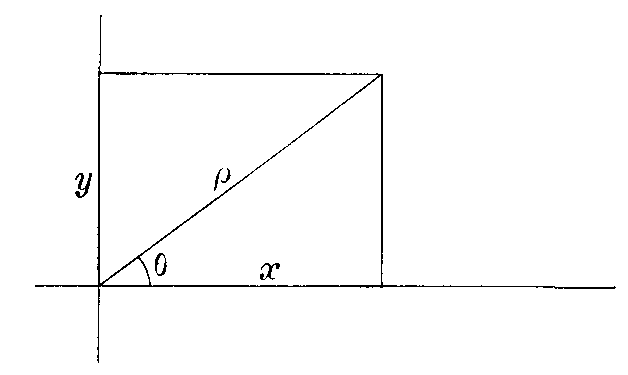
\includegraphics[width=60mm]{fig61.png}
\end{figure}

\begin{description}
\item[1.~極座標と直交座標の関係:]\hfill\break

原点で動径が軸となす角は余角である。二つの直角三角形から、
\begin{align*}
\tan ix &= \cos\theta \tan i\rho, \\
\tan iy &= \sin\theta \tan i\rho. \\
\intertext{したがって、}
\tan^2 i\rho &= \tan^2 ix + \tan^2 iy, \\
\tan\theta &= \frac{\tan iy}{\tan ix}.
\end{align*}

\begin{figure}[h]
\centering
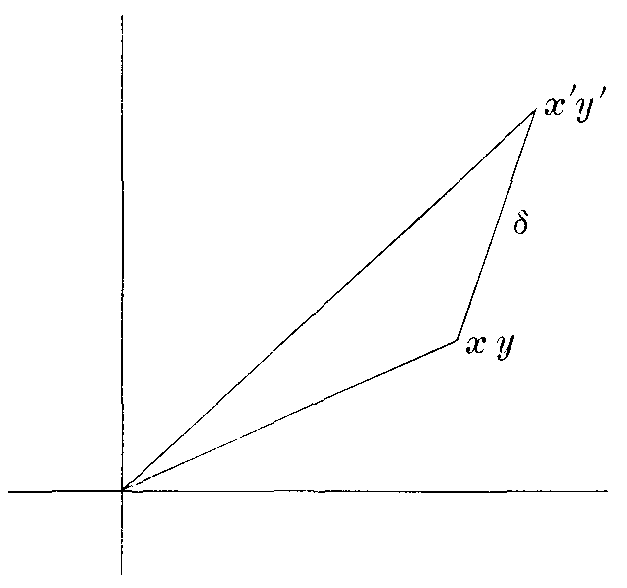
\includegraphics[width=60mm]{fig62.png}
\end{figure}

\item[2.~二点間の距離 \boldmath$\delta$:]

\begin{equation*}
\cos i\delta = \cos i\rho\, \cos i\rho'
                + \sin i\rho\, \sin i\rho'\, \cos(\theta'-\theta).
\end{equation*}
$\delta$ と一方の点を固定すれば、これは円の極方程式とみなせる。

\begin{figure}[h]
\centering
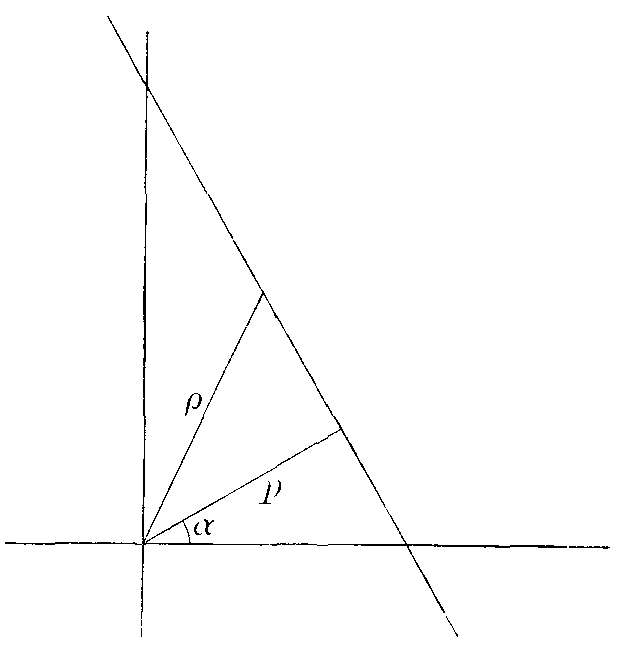
\includegraphics[width=60mm]{fig63.png}
\end{figure}

\item[3.~直線の方程式:]\hfill\break

\textbf{$p$} を原点から直線に下ろした垂線の長さ、$\alpha$ をこの垂線が $x$ 軸となす角とする。この垂線と $\rho$ でできる直角三角形から、
\begin{equation*}
\tan i\rho\, \cos(\theta-\alpha) = \tan ip
\end{equation*}
を得る。これは直線の極方程式である。展開して代入することにより、$x$ と $y$ の方程式
\begin{equation*}
\cos\alpha\,\tan ix + \sin\alpha\,\tan iy = \tan ip
\end{equation*}
を得る。

方程式 $a\tan ix + b\tan iy = i$ は、
\begin{equation*}
a^2 + b^2 = \frac{-1}{\tan^2 ip}
\end{equation*}
である直線を表す。ところで、$p$ の実数値に対して $-\tan^2ip < 1$ である（前出の脚注を見よ）。したがって直線が実であるのは、$a$ と $b$ が実数で、
\begin{equation*}
a^2 + b^2 > 1
\end{equation*}
であるときである。

\begin{figure}[h]
\centering
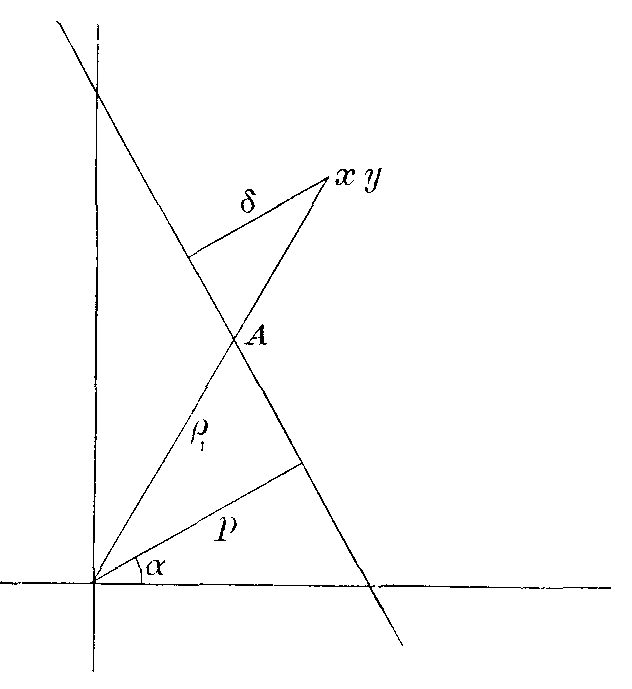
\includegraphics[width=60mm]{fig64.png}
\end{figure}

\item[4.~点から直線までの距離 \boldmath$\delta$:]\hfill\break

その点への動径が直線と $A$ で交わるとし、$\rho_1$ を $A$ への動径とする。$A$ で等しい角をもつ二つの直角三角形があり、これらの角の正弦の表式から方程式
\begin{equation*}
\frac{\sin i\delta}{\sin i(\rho-\rho_1)} =
                                        \frac{\sin ip}{\sin i\rho_1}
\end{equation*}
を得る。この方程式は平面のすべての点 $x\,y$ について成り立つ。$\delta$ は、点が原点と直線の同じ側にあるときは負であり、点が直線上にあるときは零である。
\begin{equation*}
\sin i\delta
   =\frac{\sin ip}{\tan i\rho_1}\sin i\rho-\sin ip\,\cos i\rho.
\end{equation*}

さて、
\begin{align*}
\tan i\rho_1 &= \frac{\tan ip}{\cos(\theta-\alpha)}. \\
\therefore \frac{\sin ip}{\tan i\rho_1}\sin i\rho
           &=\sin i\rho\,\cos ip\,\cos(\theta-\alpha), \\
\intertext{および}
 \sin i\delta &= \cos i\rho\, \cos ip\,
   \left[\tan i\rho\, \cos(\theta-\alpha) - \tan ip\right].
\end{align*}
$\delta$ を固定すれば、これは等距離曲線の極方程式とみなせる。

\begin{figure}[ht]
\centering
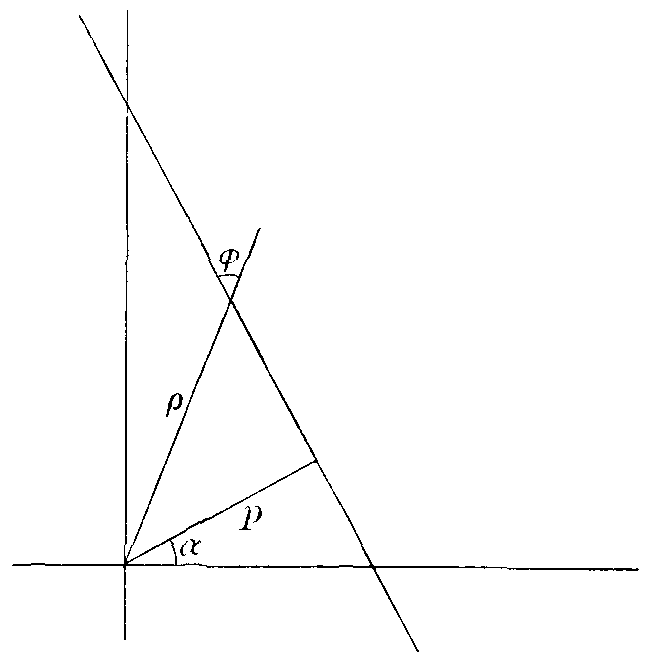
\includegraphics[width=60mm]{fig65.png}
\end{figure}

\item[5.~二直線のなす角:]\hfill\break

$\phi$ を、直線が任意の点で動径となす角とすると、
\begin{align*}
 \cos \phi &= \cos ip\, \sin (\theta-\alpha),\\
 \sin \phi &= \frac{\sin ip}{\sin i\rho}.
\end{align*}

この点で交わる二直線については、
\begin{align*}
 \sin \phi_1\, \sin \phi_2 &= \frac{\sin ip_1\, \sin ip_2}{\sin^2 i\rho}\\
 &= \sin ip_1\, \sin ip_2 + \frac{\sin ip_1\, \sin ip_2}{\tan^2 i\rho}.
\end{align*}

さて、直線の方程式から、
\begin{align*}
\frac{\sin ip_1}{\tan i\rho} &= \cos ip_1\, \cos(\theta-\alpha_1),\\
\frac{\sin ip_2}{\tan i\rho} &= \cos ip_2\, \cos(\theta-\alpha_2);\\
\intertext{したがって}
\sin \phi_1 \sin \phi_2 &= \sin ip_1\, \sin ip_2
   + \cos ip_1\, \cos ip_2\, \cos(\theta-\alpha_1)\,\cos(\theta-\alpha_2).\\
\intertext{またさらに、}
\cos \phi_1\, \cos \phi_2 &= \cos ip_1\, \cos ip_2\, \sin
  (\theta-\alpha_1)\,\sin (\theta-\alpha_2). \\
\intertext{これらの式を加えると、}
\cos (\phi_2-\phi_1) &= \sin ip_1\, \sin ip_2 +
        \cos ip_1\, \cos ip_2\, \cos (\alpha_2-\alpha_1).
\end{align*}

二直線が垂直であるのは、
\begin{align*}
\cos (\alpha_2-\alpha_1) + \tan ip_1\, \tan ip_2 &= 0 \\
\intertext{のときである。直線}
 a \tan ix + b \tan iy &= i,\\
 a' \tan ix + b' \tan iy &= i, \\
\intertext{が垂直であるのは、}
aa' + bb' &=1
\end{align*}
のときである。

\item[6.~円の $x$ と $y$ による方程式:]

\begin{align*}
 \sin i\rho\, \cos \theta &= \cos i\rho\, \tan ix,\\
 \sin i\rho\, \cos \theta &= \cos i\rho\, \tan iy;
\intertext{また、}
 \cos i\rho &= \frac{1}{\sqrt{1+\tan^2 i\rho}} =
\frac{1}{\sqrt{1+\tan^2 ix+\tan^2 iy}}.
\end{align*}

したがって、円の方程式は次のように書ける。
\begin{multline*}
  (1 + \tan^2ix + \tan^2iy)
  (1 + \tan^2ix' + \tan^2iy') \cos^2i\delta\\
  = (1 + \tan ix \tan ix' + \tan iy \tan iy')^2.
\end{multline*}

\begin{figure}[h]
\centering
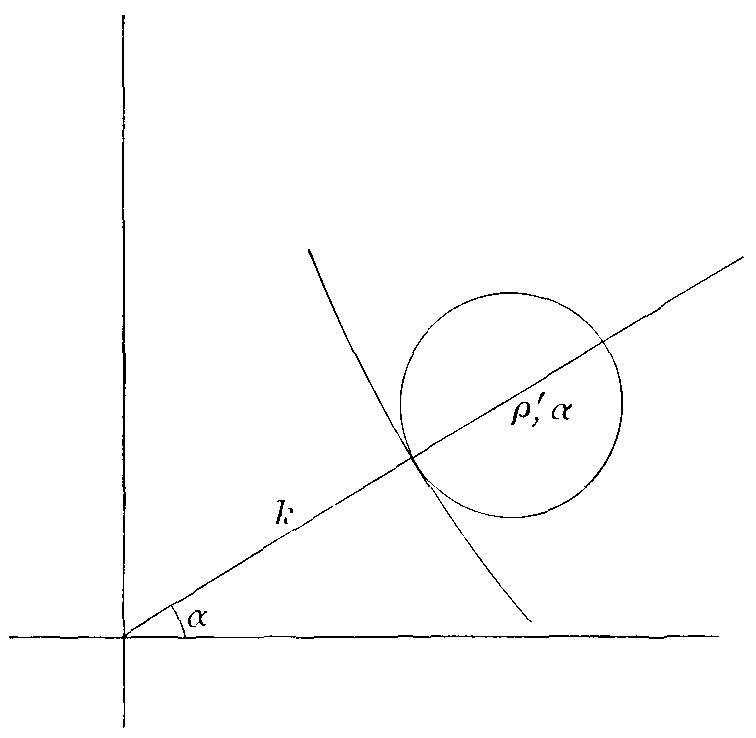
\includegraphics[width=60mm]{fig66.png}
\end{figure}

\item[7.~限界曲線の方程式:]\hfill\break

\textbf{原点}を通る限界曲線の軸が $x$ 軸と角 $\alpha$ をなすとし、限界曲線がこの軸と交わる点が原点から距離 $k$ にあるとする。$k$ は、原点が曲線の凸の側にあるときは正、曲線の凹の側にあるときは負とする。限界曲線は、この軸上の中心が限りなく遠ざかるときの円の極限の位置である。

$\rho'$ を中心への動径とすると、円の半径は $\rho'-k$ であり、その方程式は
\begin{equation*}
  \cos i(\rho'-k) = \cos i\rho\, \cos i\rho'
  + \sin i\rho\, \sin i\rho'\, \cos(\theta-\alpha)
\end{equation*}
と書ける。あるいは、展開して $\cos i\rho'$ で割ると、
\begin{equation*}
  \cos ik + \tan i\rho'\, \sin ik
  = \cos i\rho + \sin i\rho\, \tan i\rho'\, \cos(\theta-\alpha).
\end{equation*}

ここで $\rho'$ を限りなく増加させる。$\tan i\rho'$ は極限 $i$ に近づくから、この式の左辺の極限は、
\begin{equation*}
  \cos ik + i\sin ik, \text{ すなわち } e^{-k}
\end{equation*}
であり、曲線の極方程式は、
\begin{equation*}
  e^{-k} = \cos i\rho \left[1 + i\tan i\rho\,\cos(\theta-\alpha) \right]
\end{equation*}
となる。あるいは $x\,y$ 座標では、
\begin{equation*}
  (1 + \tan^2ix + \tan^2iy) e^{-2k}
     = (1 + i\cos\alpha\,\tan ix + i\sin\alpha\,\tan iy)^2.
\end{equation*}

\begin{figure}[h]
\centering
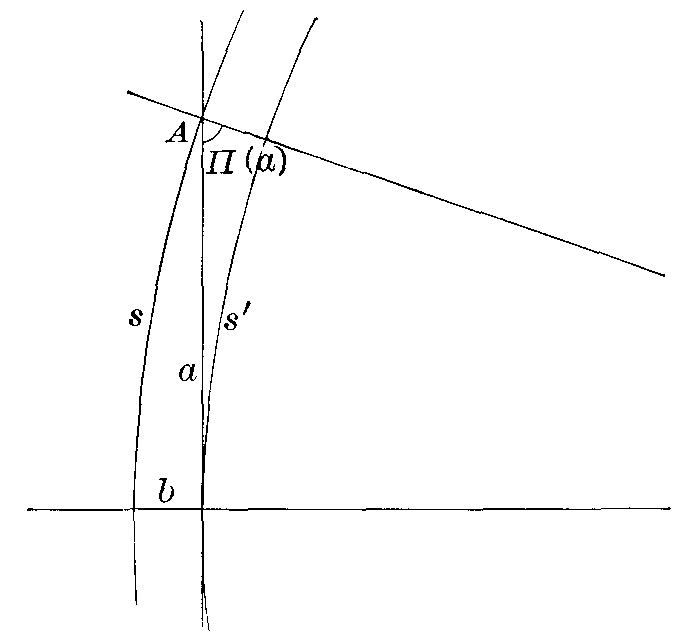
\includegraphics[width=60mm]{fig67.png}
\end{figure}

\textbf{$k$} が負で、たとえば $-b$ に等しいとし、$\alpha=0$ とする。また、$a$ を、曲線が $y$ 軸と交わる点 $A$ の縦座標とする。

方程式に代入すると、
\begin{equation*}
  e^b = \cos ia
\end{equation*}
を得る。

$A$ を通って $x$ 軸に平行に、したがって $y$ 軸と角 $\Pi(a)$ をなす直線を引く。同じ平行線の組を軸とする限界曲線を原点を通って引き、二つの限界曲線がこれらの軸上に距離 $b$ を切り取るようにすれば、対応する弧の比は
\begin{gather*}
  \frac{s'}{s} = \sin\Pi(a) = \frac{1}{\cos ia};
\tag{前出を見よ} \\
\intertext{であることがわかっている。したがって、}
  \frac{s'}{s} = e^{-b}.\tag{前出を見よ}
\end{gather*}

\item[8.~等距離曲線の方程式:]\hfill\break

(4) の極方程式を $x$ と $y$ の方程式に直すと、次の形になる。
\begin{multline*}
  (1 + \tan^2ix + \tan^2iy) \sin^2i\delta \\
  = \cos^2ip (\cos\alpha\,\tan ix + \sin\alpha\, \tan iy -\tan ip)^2.
\end{multline*}

\item[9.~三つの方程式の比較:]\hfill\break

方程式
\begin{equation*}
  (1 + \tan^2ix + \tan^2iy)c^2
     = -(i-a\tan ix -b\tan iy)^2
\end{equation*}
は、それぞれ $a^2+b^2 < 1$、$=1$、$>1$ に応じて、円、限界曲線、等距離曲線を表す。

\begin{figure}[h]
\centering
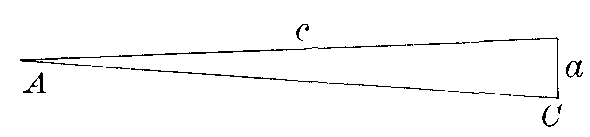
\includegraphics[width=60mm]{fig68.png}
\end{figure}

\item[10.~微分公式:]\hfill\break

頂点の角 $A$ が限りなく小さくなる二等辺三角形を考える。公式
\begin{equation*}
  \frac{\sin A}{\sin ia} = \frac{\sin C}{\sin ic}
\end{equation*}
において、
\begin{center}
\begin{tabular}{ccc}
  $\sin A$, & $\sin ia$, & $\sin C$\\
  の代わりに $A$, & $ia$, & $1$\\
\end{tabular}\\
\end{center}
をそれぞれおくことができる。したがって、
\begin{equation*}
  ia = \sin ic \cdot A.\tag{I.}
\end{equation*}

\textbf{系.} \emph{半径 $\mathbf{r}$ の円において、任意の弧と、中心で張る角との比は $\sin \mathbf{ir}$ である。}

\begin{figure}[h]
\centering
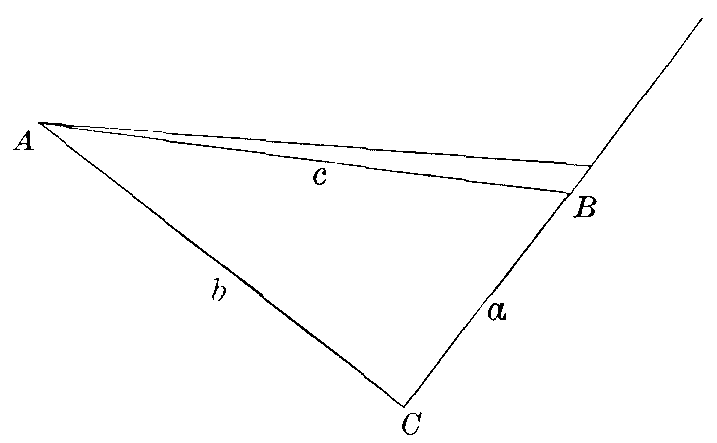
\includegraphics[width=60mm]{fig69.png}
\end{figure}

またさらに、直角三角形 $ABC$ において、斜辺 $c$ を頂点 $A$ のまわりに回転させる。方程式
\begin{align*}
\sin A &= \frac{\cos B}{\cos ib},  \\
\intertext{を（$b$ は定数として）微分すると、}
\cos Ad\,A &= -\,\frac{\sin B\,dB}{\cos ib}.  \\
\intertext{しかるに}
\sin B &= \frac{\cos A}{\cos ia};  \\
\therefore dB &= -\cos ia\, \cos ib\, dA,  \\
\intertext{すなわち（II.）}
dB &= -\cos ic\, dA.
\end{align*}

さて、極座標を用いると、斜辺 $ds$ が動径とたとえば角 $\phi$ をなす無限小の直角三角形ができる（図70を見よ）。直角をはさむ二辺は $d\rho$ と $\frac{\sin i\rho}{i} d\theta$ であるから、
\begin{align*}
ds^2 &= d\rho^2 - \sin^2i\rho\, d\theta^2,  \\
\tan\phi &= \frac{\sin i\rho}{i}\, \frac{d\theta}{d\rho}.
\end{align*}

\begin{figure}[h]
\centering
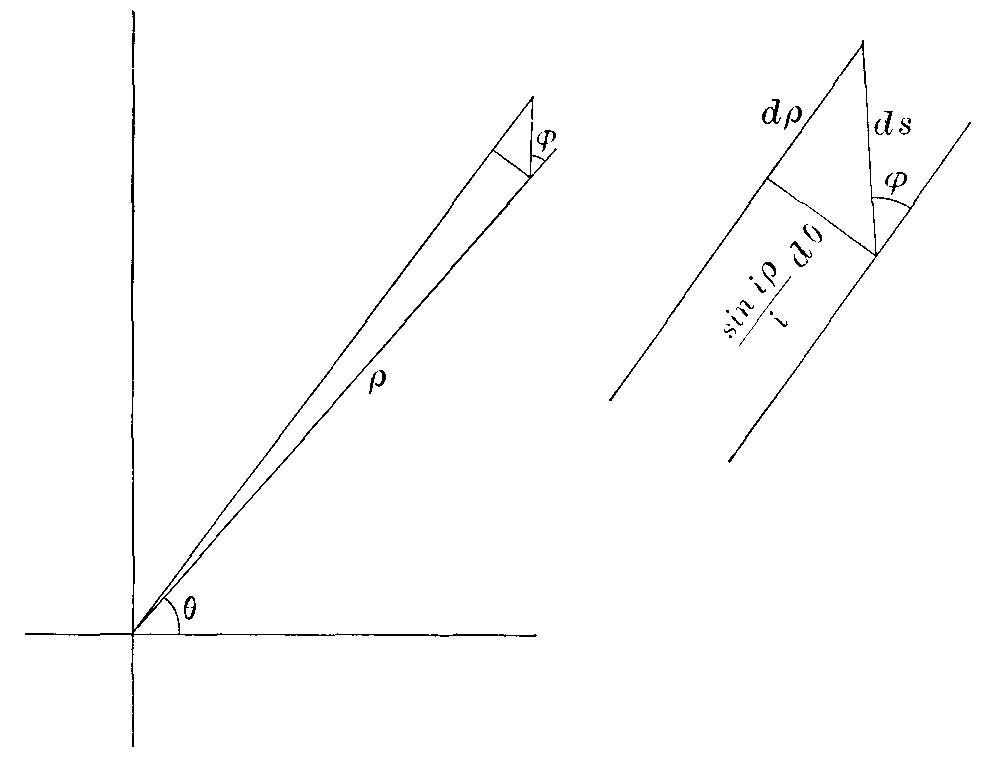
\includegraphics[width=80mm]{fig70.png}
\end{figure}

直角に交わる二つの弧について、$d'$ で第二の弧に沿った微分を表す。
\begin{align*}
  \frac{\sin i\rho}{i}\, \frac{d\theta}{d\rho}
  &= -\, \frac{i}{\sin i\rho}\, \frac{d'\rho}{d'\theta},\\
\intertext{すなわち}
  \frac{d\rho}{d\theta}\, \frac{d'\rho}{d'\theta}
  &= \sin^2i\rho.
\end{align*}

\item[11.~面積:]\hfill\break

面積は
\begin{equation*}
  \iint \frac{\sin i\rho}{i}\, d\rho\, d\theta
\end{equation*}
に等しい。\footnote{面積の単位は、無限小の長方形の面積が、その底辺と高さの積で表されるように選ぶ。}

原点が計算する面積の内部にあって、各動径が境界の曲線とただ一度だけ交わる場合のみを考える。

$\rho$ について $\rho=0$ から積分すると、
\begin{align*}
  \int_0^{2\pi} (\cos i\rho - 1) d\theta,\\
  \intertext{すなわち}
  \int_0^{2\pi} \cos i\rho\, d\theta - 2\pi
\end{align*}
を得る。

\begin{figure}[h]
\centering
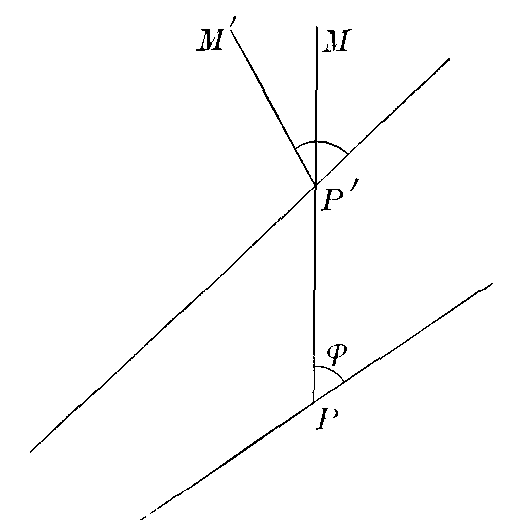
\includegraphics[width=60mm]{fig71.png}
\end{figure}

$P$ と $P'$ を曲線上の二つの「隣り合う」点とし、$PM$ と $P'M'$ をそれらの点での接線とし、$\phi$ を接線が動径となす角とする。角 $MP'M'$ は、曲線を一周するときのこれらの点での回転の量を表す。

さて、(II.) により、
\begin{equation*}
  MP'M' = d\phi + \cos i\rho\, d\theta.
\end{equation*}

曲線を一周するとき、$\phi$ は変化しうるが、最後にはもとの値に戻る。すなわち、この曲線については、
\begin{gather*}
  \int d\phi = 0, \\
\intertext{であり、回転の量は}
  \int_0^{2\pi} \cos i\rho\, d\theta
\end{gather*}
である。

ゆえに、面積は、曲線を一周するときの回転の量の、四直角を超える過剰に等しい。この定理は、任意の有限な面積に拡張できる。

\item[12.~座標系の修正:]\hfill\break

$\tan ix$ の代わりに $iu$、$\tan iy$ の代わりに $iv$、$\tan i\rho$ の代わりに $ir$ と書き、以下すべての線の長さについても同様にすると、方程式は簡単な形になる。

すると、
\begin{align*}
u^2 + v^2 &= r^2.\footnotemark \\
\intertext{直線の方程式は}
au + bv &= 1, \\
\intertext{であり、方程式}
(1 - u^2 - v^2)c^2 &= (1 - au - bv)^2
\end{align*}
は、それぞれ $a^2+b^2<1$、$=1$、$>1$ に応じて、円、限界曲線、等距離曲線を表す。
\footnotetext{三つの直角をもつ四角形を描き、鋭角への対角線を引いて、$a$、$b$、$c$ を上の $u$、$v$、$r$ と同じように用いれば、図に記した五つの部分は、ユークリッド幾何学の直角三角形の関係をもつ。たとえば、
\begin{equation*}
a^2 + b^2 = c^2 , \sin A = \frac{a}{c}, \text{など}.
\end{equation*}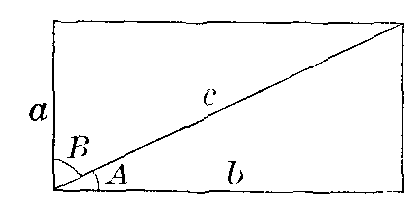
\includegraphics[width=25mm]{fig73.png}}
\end{description}


\section{楕円解析幾何学}

楕円解析幾何学は、双曲解析幾何学を展開したのとまったく同じように展開でき、公式は因子 $i$ を除いたものと同じになる。しかしこれらの公式は、直線と極の関係からも非常に容易に得られるから、そのようにして導く。

楕円平面解析幾何学の公式は、三つの幾何学のどれにおいても、球面に適用できる。

\begin{figure}[h]
\centering
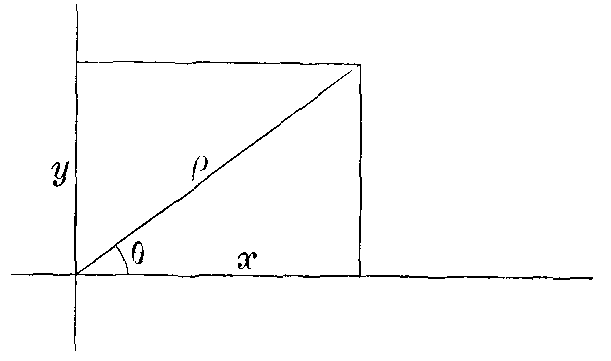
\includegraphics[width=60mm]{fig72.png}
\end{figure}

\begin{description}
\item[1.~極座標と直交座標の関係:]

\begin{gather*}
\tan x = \cos\theta\, \tan\rho, \quad \tan y = \sin\theta\, \tan\rho; \\
\intertext{したがって、}
\begin{aligned}
  \tan^2\rho &= \tan^2x + \tan^2y,\\
  \tan\theta &= \frac{\tan y}{\tan x}.\footnotemark
\end{aligned}
\end{gather*}
\footnotetext{原点を極とする直線は、座標軸とともに三直角三角形をつくり、$x$、$y$、$\theta$ は、与えられた点のそれらの三つの頂点からの方向を表すとみなしてよい。
\par 球面上で、赤道の極を原点にとれば、$\rho$ と $\theta$ は余緯度と経度である。$x$ と $y$ は、一方は符号を変えて、赤道上の $90^\circ$ 離れた二点からのその点の「方位」である。}

\begin{figure}[h]
\centering
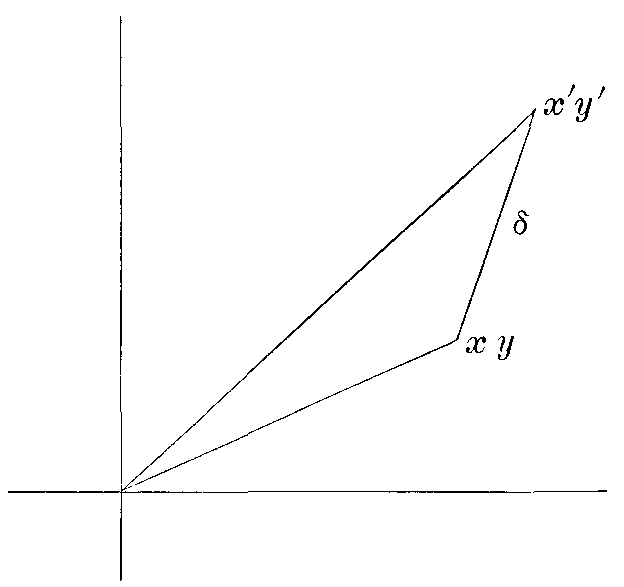
\includegraphics[width=60mm]{fig74.png}
\end{figure}

\item[2.~二点間の距離 \boldmath$\delta$:]

\begin{equation*}
\cos\delta = \cos\rho\,\cos\rho' +
                             \sin\rho\,\sin\rho'\cos(\theta'-\theta).
\end{equation*}

これは、$\rho'$ と $\theta'$ を中心の極座標とする、半径 $\delta$ の円の極方程式とみなせる。

さて、
\begin{align*}
  \sin\rho\,\cos\theta &= \cos\rho\,\tan x,\\
  \sin\rho\,\sin\theta &= \cos\rho\,\tan y;
\intertext{また、}
  \cos\rho = \frac{1}{\sqrt{1+\tan^2\rho}}
  &= \frac{1}{\sqrt{1+\tan^2x+\tan^2y}}
\end{align*}
したがって、円の直交座標による方程式は次のように書ける。
\begin{multline*}
  (1 + \tan^2x + \tan^2y) (1 + \tan^2x' + \tan^2y') \cos^2\delta\\
  = (1 + \tan x\tan x' + \tan y\tan y')^2.
\end{multline*}

\begin{figure}[h]
\centering
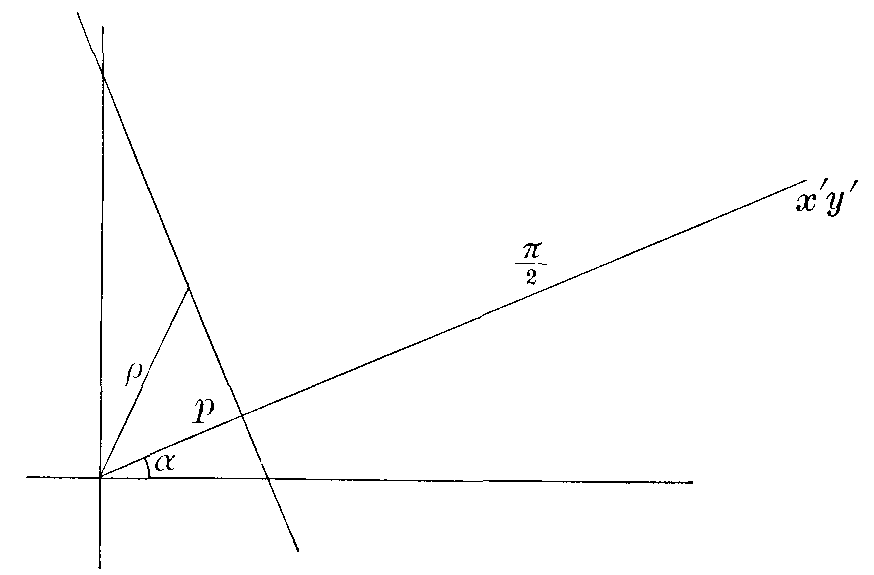
\includegraphics[width=60mm]{fig75.png}
\end{figure}

\item[3.~直線の方程式:]\hfill\break

$\delta = \frac{\pi}{2}$ のとき、円は直線になる。したがってこの場合は、方程式
\begin{equation*}
  \tan x \tan x' + \tan y \tan y' + 1 = 0
\end{equation*}
を得る。$x'y'$ は直線の極である。

方程式
\begin{align*}
\tan\rho\, \cos(\theta-\alpha) &= \tan p, \\
\intertext{すなわち}
\cos\alpha\, \tan x + \sin\alpha\,\tan y &= \tan p, \\
\intertext{から}
\tan x' &= -\frac{\cos\alpha}{\tan p},\\
\tan y' &= -\frac{\sin\alpha}{\tan p}
\end{align*}
を得る。これは幾何学的に示すこともでき、この点の極座標は
\begin{equation*}
p+\frac{\pi}{2},\ \alpha
\end{equation*}
である。

方程式
\begin{equation*}
  a\tan x + b\tan y + 1 = 0
\end{equation*}
は、$a$ と $b$ の任意の実数値に対して、実の直線を表す。

\item[4.~点から直線までの距離 \boldmath$\delta$:]\hfill\break

これは、その点と直線の極との間の距離の余角である。次の方程式で表される。
\begin{align*}
  \sin\delta &= -\cos\rho\,\sin p
                            + \sin\rho\,\cos p\,\cos(\theta-\alpha)\\
  &= \cos\rho\,\cos p
                 \left[\tan\rho\,\cos(\theta-\alpha) - \tan p\right].
\end{align*}

\item[5.~二直線のなす角 \boldmath$\phi$:]\hfill\break

これはそれらの極の間の距離に等しい。したがって、
\begin{equation*}
  \cos\phi = \sin p\,\sin p' + \cos p\,\cos p'\,\cos(\alpha'-\alpha).
\end{equation*}

二直線
\begin{align*}
  a\phantom{'}\tan x + b\phantom{'}\tan y + 1 &= 0,\\
  a'\tan x + b'\tan y + 1 &= 0\\
  \intertext{が垂直であるのは、}
  aa' + bb' + 1 &= 0
\end{align*}
のときである。

\begin{figure}[h]
\centering
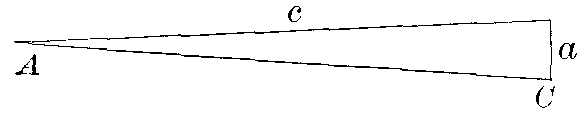
\includegraphics[width=60mm]{fig76.png}
\end{figure}

\item[6.~微分公式:]\hfill\break

公式
\begin{equation*}
  \frac{\sin A}{\sin a} = \frac{\sin C}{\sin c}
\end{equation*}
は、$A$ が限りなく小さくなるとき、
\begin{equation*}
  a = \sin c \cdot A\tag{I.}
\end{equation*}
となる。

\textbf{系.} \emph{半径 $\mathbf{r}$ の円において、任意の弧と、中心で張る角との比は $\sin \mathbf{r}$ である。}

\begin{figure}[h]
\centering
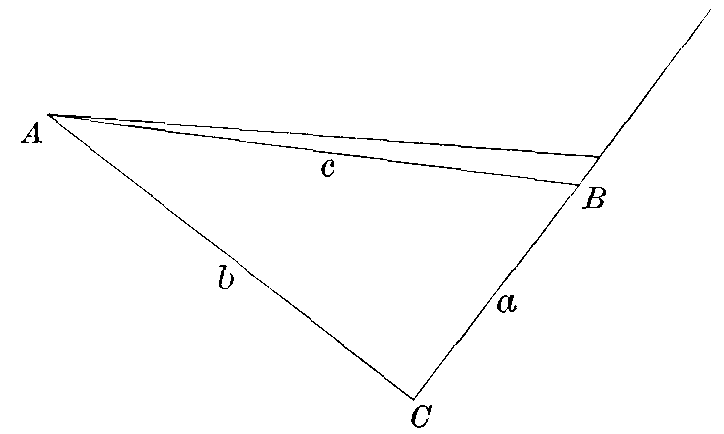
\includegraphics[width=60mm]{fig77.png}
\end{figure}

直角三角形 $ABC$ から、$b$ を固定したままにして、方程式
\begin{align*}
  \sin A &= \frac{\cos B}{\cos b}
\intertext{を微分すると、}
  dB &= -\cos c \,dA\tag{II.}
\end{align*}
を得る。

\begin{figure}[h]
\centering
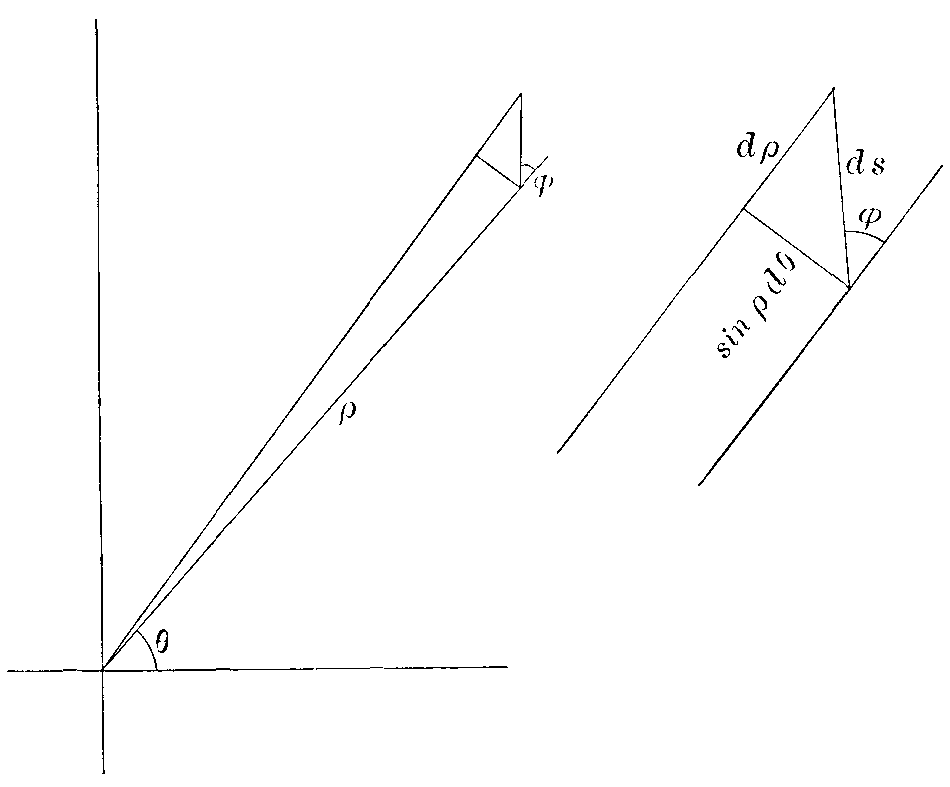
\includegraphics[width=80mm]{fig78.png}
\end{figure}

こうして、極座標での微分公式は、
\begin{align*}
  ds^2 &= d\rho^2 + \sin^2\rho\,d\theta^2,\\
  \tan\phi &= \sin\rho\, \frac{d\theta}{d\rho};\footnotemark
\intertext{直角に交わる二つの弧については}
  \frac{d\rho}{d\theta}\, \frac{d'\rho}{d'\theta} &= -\sin^2\rho
\end{align*}
である。
\footnotetext{ユークリッド幾何学の対数螺旋のように $\phi$ が定数であれば、この方程式を積分することができる。すなわち、
  \begin{align*}
    \tan\phi\, \frac{d\rho}{\sin\rho} &= d\theta.\\
    \therefore \tan\phi\, \log\tan\frac{\rho}{2} &= \theta+c,\\
    \intertext{すなわち}
    \tan\frac{\rho}{2} &= e^\frac{\theta+c}{\tan\phi}.\\
    \intertext{$e^\frac{c}{\tan\phi}$ を $c'$ と書くと、これは}
    \tan\frac{\rho}{2} &= c' e^\frac{\theta}{\tan\phi}
  \end{align*}
  となる。球面上では、これは斜航線と呼ばれる曲線である。}

面積の公式は、\footnote{面積の単位を適切に選ぶ。}
\begin{equation*}
  \iint \sin\rho\, d\rho\, d\theta
\end{equation*}
である。まず $\rho$ について積分する。面積が原点を含み、各動径が曲線とただ一度だけ交わるならば、この式は
\begin{equation*}
  2\pi - \int_0^{2\pi} \cos\rho\, d\theta
\end{equation*}
となる。

曲線を一周するときの全回転は、双曲の場合と同様にして求められ、
\begin{equation*}
  \int_0^{2\pi} \cos\rho\, d\theta
\end{equation*}
である。したがって、面積は、この回転が四直角に足りない量に等しい。

たとえば、半径 $\rho$ の円の面積は $2\pi(1-\cos\rho)$ であり、その一周で回転する量は $2\pi\cos\rho$ である。平面全体の面積は $2\pi$ である。

\item[7.~座標系の修正:]\hfill\break

$\tan x$ の代わりに $u$、$\tan y$ の代わりに $v$、$\tan\rho$ の代わりに $r$、などと書くと、
\begin{align*}
  u^2 + v^2 &= r^2.\footnotemark \\
\intertext{直線の方程式は}
  au + bv + 1 &= 0, \\
\intertext{となり、円の方程式は}
  (1 + u^2 + v^2)c^2 &= (1 + au + bv)^2
\end{align*}
となる。
\footnotetext{双曲の場合の脚注はここにも当てはまる。}
\end{description}


\section{楕円立体解析幾何学}

二重回転面の方程式が得られるところまで展開する。

\begin{figure}[h]
\centering
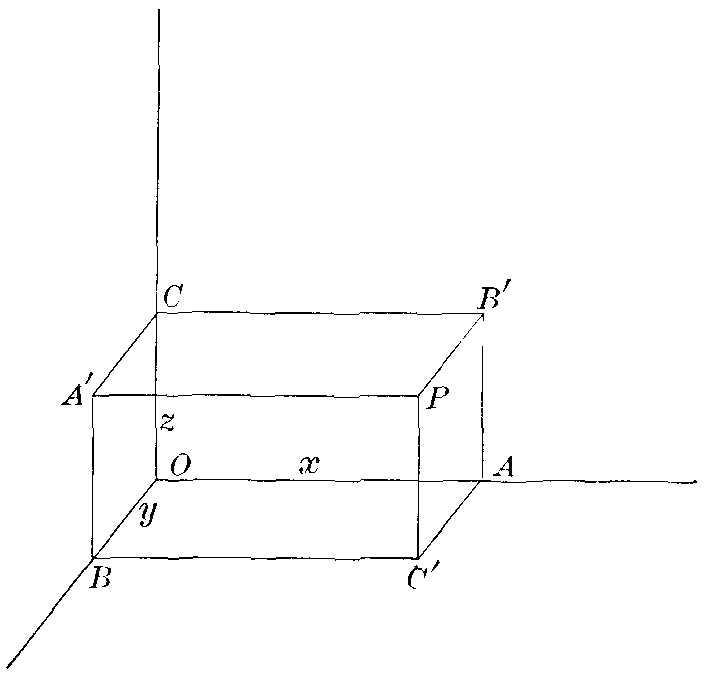
\includegraphics[width=60mm]{fig79.png}
\end{figure}

\begin{description}
\item[1.~座標、直線、平面:]\hfill\break

点を通って軸に垂直な三つの平面を引く。座標 $x$、$y$、$z$ としては、これらの平面が軸上に切り取る切片をとる。

これら三つの平面の交線は、座標平面に垂直である（第I章, II, 16 および 17）。実際、図の面角はすべて直角であるが、$P$ での角と、三つの角 $BA'C$、$CB'A$、$AC'B$ は鈍角である。

$\rho$ を点 $P$ への動径とし、$\alpha$、$\beta$、$\gamma$ をそれが三つの軸となす三つの角とする。すると、
\begin{align*}
  \cos^2\alpha + \cos^2\beta + \cos^2\gamma &= 1,\\
  \cos\alpha &= \frac{\tan x}{\tan\rho},\ \text{など;}\\
  \tan^2x + \tan^2y + \tan^2z &= \tan^2\rho.
\end{align*}

原点で交わる二直線のなす角については、
\begin{equation*}
  \cos\theta = \cos\alpha\,\cos\alpha' + \cos\beta\,\cos\beta'
  + \cos\gamma\,\cos\gamma'.
\end{equation*}

二点 $xyz$ と $x'y'z'$ が原点で張る角は、方程式
\begin{equation*}
  \cos\theta = \frac{\tan x\, \tan x' + \tan y\, \tan y'
    + \tan z\, \tan z'}{\tan\rho\, \tan\rho'}
\end{equation*}
で与えられる。

二点間の距離については、
\begin{equation*}
  \cos\delta = \cos\rho\,\cos\rho' + \sin\rho\,\sin\rho'\,\cos\theta.
\end{equation*}

これから球面の方程式が得られ、$\delta = \frac{\pi}{2}$ のとき平面の方程式が得られる。後者を直交座標で表すと、
\begin{equation*}
  \tan x\, \tan x' + \tan y\, \tan y' + \tan z\, \tan z' + 1 = 0
\end{equation*}
である。

$p$ を原点から平面に下ろした垂線の長さとし、$\alpha$、$\beta$、$\gamma$ をこの垂線が軸となす角とする。するとその極については、
\begin{align*}
  \rho' &= p + \frac{\pi}{2},\\
  \tan x' = \tan\rho'\,\cos\alpha &= -\,\frac{\cos\alpha}{\tan p},\
  \text{など;}
\end{align*}
ゆえに、平面の方程式は次のように書ける。
\begin{equation*}
\cos\alpha\,\tan x + \cos\beta\,\tan y + \cos\gamma\,\tan z
   = \tan p.
\end{equation*}

\item[2.~二重回転面:]\hfill\break

その軸の一つを $z$ 軸にとり、$k$ を曲面からこの軸までの距離とし、$\theta$ を、点 $P$ と $z$ 軸を通る平面が $xz$ 平面となす角とする。$z$ と $\theta$ を緯度と経度と呼ぶことができる。

$OA$ と $CB$ を延長する。それらは、$z$ 軸から距離 $\frac{\pi}{2}$ のところで、曲面の他方の軸上の点 $O'$ で交わり、そこで測度が $z$ に等しい角をなす。

直角三角形 $O'AB$ から、
\begin{align*}
\cos z &= \frac{\tan OA}{\tan O'B}.\\
\intertext{しかるに}
\tan O'A &= \cot x,\\
\intertext{および}
\tan O'B &= \cot CB = \frac{\cot k}{\cos\theta}.\\
\intertext{したがって、}
\cos z &= \frac{\tan k\,\cos\theta}{\tan x},\\
\intertext{すなわち}
\tan x &= \frac{\tan k\,\cos\theta}{\cos z}.\\
\intertext{同様にして、}
\tan y &= \frac{\tan k\,\sin\theta}{\cos z}.\\
\intertext{二乗して加えると、曲面の方程式は}
\tan^2x + \tan^2y &= \tan^2k\sec^2z
\end{align*}
となる。

\begin{figure}[h]
\centering
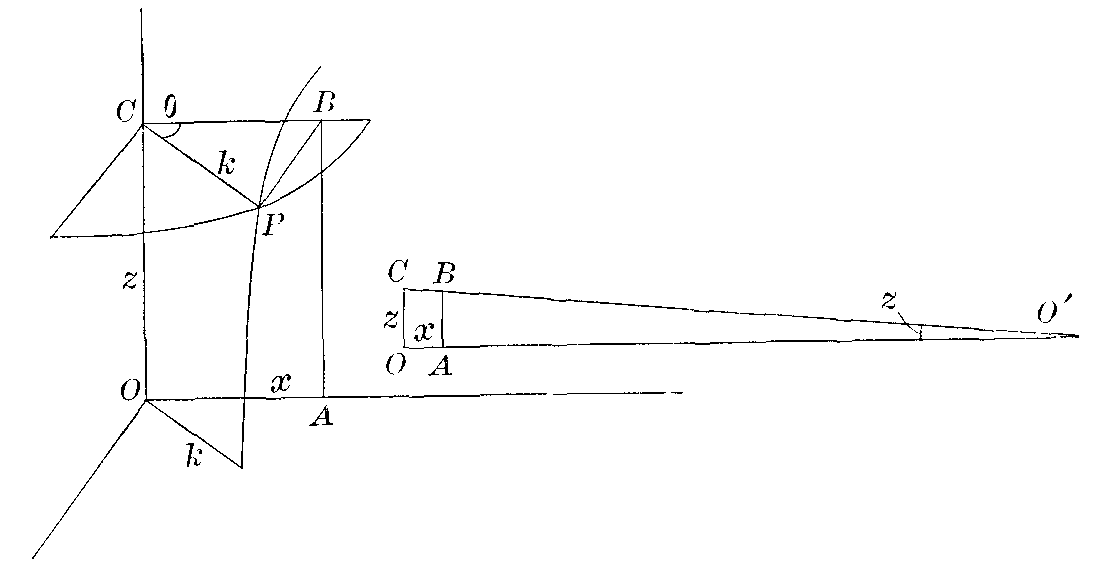
\includegraphics[width=80mm]{fig80.png}
\end{figure}

曲面上の二点を結ぶ弦の長さについては、
\begin{equation*}
\cos\delta = \cos\rho\,\cos\rho'
  (1 + \tan x\,\tan x' + \tan y\,\tan y' + \tan z\,\tan z').
\end{equation*}
さて、
\begin{align*}
\tan^{2}\rho &= \tan^{2}k\,\sec^{2}z + \tan^{2}z; \\
\intertext{したがって、}
\sec^{2}\rho &= \sec^{2}k\,\sec^{2}z,\\
\intertext{すなわち}
\cos\rho &= \cos k\,\cos z. \\
\intertext{すなわち、$z$、$z'$、$\theta$、$\theta'$ で表すと、}
\cos\delta &= \cos^2k\,\cos(z'-z) + \sin^2k\,\cos(\theta'-\theta). \\
\intertext{これから、曲面上の長さの微分要素 $ds$ の表式が得られる。}
\cos ds &= \cos^2k\,\cos dz + \sin^2k\,\cos d\theta, \\
\intertext{あるいは、}
\cos ds &= 1 - \frac{ds^2}{2},\ \text{など,} \text{ であるから} \\
ds^2 &= \cos^2k\, dz^2 + \sin^2k\, d\theta^2.
\end{align*}

$z$ と $\theta$ は、二つの円の系に沿って測った距離に比例する。これらの円は直角に交わり、曲面上の直交座標系を与えるのに用いることができる。これら二つの円の系に沿った実際の長さは $\theta\sin k$ と $z\cos k$ である（第III章の系を見よ）。したがって、
\begin{equation*}
\alpha = \theta\sin k,\quad \beta = z\cos k
\end{equation*}
と書けば、直角に交わるこれら二つの円の系に沿って測った距離を座標とする、曲面上の直交系が得られる。

公式はこのとき
\begin{equation*}
ds^2 = d\alpha^2 + d\beta^2
\end{equation*}
となる。

$\alpha$ と $\beta$ の一次方程式は、この曲面上で、ユークリッド幾何学の平面上の直線のすべての性質をもつ曲線を表す。任意の二点を通って、そのような線がただ一本引ける。二組の座標は、一次方程式の係数を決めるのにちょうど十分だからである。曲面上の二点間の最短距離は、そのような線上で測られる。なぜなら、$\alpha$ と $\beta$ の方程式で表される道に沿った二点間の距離は、$\alpha$ と $\beta$ を直交座標にとったユークリッド平面上の、対応する点と対応する道に沿った距離と同じだからである。したがって、道が $\alpha$ と $\beta$ の一次方程式で表されるときに、それが最短でなければならない。曲面上のそのような線を\emph{測地線}といい、曲面に関するかぎり、直線と呼ぶ。これらの線の一つの上で測った任意の二点間の距離は、公式
\begin{equation*}
d = \sqrt{(\alpha-\alpha')^2 + (\beta-\beta')^2}
\end{equation*}
で表される。

これらの線でつくられる三角形は、ユークリッド幾何学の平面三角形のすべての性質をもつ。角の和は $\pi$ である、などである。実際、この曲面と楕円空間との関係は、限界面と双曲空間との関係と同じである。

直線の方程式の標準形は、
\begin{equation*}
\alpha\cos\omega + \beta\sin\omega = p
\end{equation*}
である。

曲面の直線の母線は、$z$ 軸の極線である軸のまわりに描いたすべての円と、一定の角 $\pm k$ をなす。したがってこれらの母線は曲面上の「直線」であり、その方程式は次の形になる。
\begin{equation*}
\alpha\cos k \pm \beta\sin k = p.
\end{equation*}
\end{description}


\chapter{歴史的注}

非ユークリッド幾何学の歴史は、すでに非常によく、しばしば書かれているので、ここでは簡単な概略だけを述べる。

ユークリッドの公理のなかに、表現がいくぶん複雑で、他のもののような単純で初歩的な事実とは思えないものが一つある。それは次のものである。\footnote{ポール・タンヌリーによる、ユークリッドの公理についての論文を見よ。\emph{Bulletin des Sciences Mathématiques}, 1884.}

\begin{quotation}\emph{二直線が第三の直線で切られ、その切る線の同じ側の内角の和が二直角より小さいならば、二直線は十分に延長すれば、その側で出会う。}\end{quotation}

多くの数学者、とりわけルジャンドルが、この命題の証明を与えようと試みた。すなわち、それがそれに先立つより単純な公理の必然的な帰結であることを示そうとした。ルジャンドルは、三角形の角の和は決して二直角を超えないこと、また、この和が二直角に等しい三角形が一つでもあれば、すべての三角形についてそうであることを証明した。これはもちろん、直線が無限の長さをもつという仮定のもとでのことであった。しかし彼は、角の和が二直角であるような三角形が存在することを証明できなかった。\footnote{たとえば、彼の\emph{幾何学原論}（\emph{Éléments de Géométrie}）の第12版、第I巻、命題XIX、および注II を見よ。また、\emph{Bulletin des Sciences Mathématiques} 第一シリーズ第二巻の、非ユークリッド幾何学についての論文におけるクラインの言明も見よ。}

ついに、この言明は証明できないものであり、それがつねに真であるとは限らないと仮定しても、同じように無矛盾な幾何学を築き上げることができる、さらにはユークリッドのすべての公準は、われわれの経験によって真と受け入れるに至った仮説にすぎず、論理的な幾何学の展開においては反対の言明で置き換えうるものである、と考える数学者が現れはじめた。

この理論の端緒は、ときにガウスに帰せられてきたが、いまでは、1766年にランベルト\footnote{\emph{American Mathematical Monthly}, 1895年7--8月号を見よ。}が、平行線公理には証明が必要であると主張し、この公理が成り立たない幾何学の特徴のいくつかを与えた論文を書いていたことが知られている。さらに1733年という昔にも、イタリア人サッケーリが一冊の本を出版し、そこで非ユークリッド幾何学の完全な体系を与え、そのうえで、これらの他の仮説は偽であると独断的に断言することによって、自分自身とその本を救った。本書の第一章の基礎としてとられているのは、彼の取り扱いの方法である。\footnote{ハルステッドによるサッケーリの翻訳は、\emph{American Mathematical Monthly} に連載されてきた。}

ガウスは長年、平行線の公理を証明しようと努めていた。この公理を否定した帰結である定理のいくつかを発見していたかもしれないが、この主題について何も公表しなかった。

ロシアのロバチェフスキーとハンガリーのヨハン・ボヤイが、はじめて、平行線の公理が必ずしも真ではないことを主張し、証明した。二人の仕事は互いにまったく独立であり、それぞれがこの発見の全面的な功績を有する。彼らの結果は1830年ごろに公表された。

これらの発見が多くの注目を集めるまでには、長い時間がかかった。そのあいだに、後にわれわれの主題に多くの光を投げかけることになる、他の方面の研究が進められていた。それは説明としてではなく、顕著な類似によってであった。

たとえば、一、二年の間隔をおいて、同じ雑誌（クレレ）に、ロバチェフスキーの研究結果を述べた論文と、ミンディングの曲面についての論文が現れた。ミンディングは、$a$ などの代わりに $ia$ とおけば、球面三角法の公式が成り立つような曲面を見いだしたのである。しかし、これら二つの論文は、それらの関連が（ベルトラミによって）気づかれるまでに、三十年間も公表されたままであった。

またケイリーは、1859年に\emph{Philosophical Transactions} に「第六論文（量子論）」を発表し、そこで測定の射影的理論を展開して、あらゆる図形が、彼が絶対形と呼んだある特別な図形との間でもつ非調和関係を考えることにより、計量的性質を射影的に扱いうることを示した。1872年にクラインがこの理論を取り上げ、それが非ユークリッド幾何学の完全な像を与えることを示した。

また、平面や空間のなかを動き回るにつれて、ある法則に従って変化する測定の単位を考えれば、非ユークリッド幾何学が得られることも示されている。

これらの分野の古い研究者たちは、鋭角の仮説をとる幾何学だけを発見した。直線が有限の長さをもつという仮定を調べることは、彼らには思い浮かばなかった。楕円幾何学は、1854年に幾何学の基礎の研究に取り組んだリーマンによって発見されるまで、残されていた。彼はそれを、まったく異なる観点、抽象的な代数的観点から研究した。われわれの空間や幾何学的図形は、例示のためにあげるにとどめて、変数の系を考えたのである。彼は、これらの変数の関数で、長さあるいは距離の要素と呼べるものの性質はどのようなものか、という問題を調べ、最も簡単な場合には、それは、変数の微分の二次式の平方根でなければならず、その係数はそれ自身変数の関数でありうることを見いだした。二次式の異なる形をとることにより、これらの異なる種類の幾何学が無数に得られるが、そのほとんどでは、物体は大きさも形も変えずに動かせるという公理を失う。

この概観には、さらに二つの名前を加えるべきである。ヘルムホルツとクリフォードである。彼らは科学雑誌に論文を発表して、この主題を広く知らしめるのに大いに貢献した。楕円空間における平行線の理論は、前に説明したとおり、クリフォードに負っている。彼は、この幾何学のなかに、ユークリッド幾何学が成り立つ有限な曲面がありうることを示した。\footnote{非ユークリッド幾何学のより興味深い解説のいくつかは次のとおりである。\emph{Encyclopedia Britannica}、サー・ロバート・ボールによる項目「測定」（``Measurement''）。\emph{Revue Générale des Sciences}, 1891、ポアンカレによる「非ユークリッド幾何学」（``Les Géométries Non-Euclidean''）。\emph{Bulletin of the American Mathematical Society}, 1900年5月および6月、フレデリック・S・ウッズによる「ロバチェフスキーの幾何学」（``Lobachevsky's \emph{Geometry}''）。\emph{Mathematische Annalen}, Bd.~xlix, p.~149, 1897、および\emph{Bulletin des Sciences Mathématiques}, 1897、「ガウスとボヤイの書簡」（``Letters of Gauss and Bolyai''）。とくに興味深いのは、互いに平行な三本の直線が、つねに同じ有限の面積を囲むことができるという仮説のもとでの三角形の面積の公式を、ガウスが与えている一通の手紙である。最後の二つの論文は、エンゲル教授とシュテッケル教授の出版物に言及しており、それらはドイツ語で、平行線の理論の完全な歴史と、ロバチェフスキーおよびボヤイの著作と生涯を与えている。また、ジョージ・ブルース・ハルステッド教授による、ロバチェフスキーとボヤイの翻訳、およびヴァシリエフ教授の講演の翻訳も見よ。}

非ユークリッド幾何学の主な教訓は、幾何学の公理は、物理科学の理論のように、われわれの経験からの演繹にすぎないということである。数学者にとって、それらは真偽が彼の関知するところではなく、哲学者のみに関わる仮説である。彼はそれらを望む形でとり、その上に幾何学を築いてよく、こうして得られた幾何学は、数学の他の分野に応用をもつ。

これらの幾何学的命題に適用されるかぎり、「公理」は「自明」ではなく、必ずしも真ではない。ある言明が証明できる、すなわち、すでに採用された公理の必然的帰結であるならば、それを公理と呼ぶべきではない。互いに矛盾する二つ以上の言明が、すでに受け入れた公理のすべてと同じように無矛盾であるときには、そのどちらをとってもよく、われわれが選んだ言明が、われわれの幾何学にとっての公理となる。われわれの幾何学とは、この公理の帰結の研究である。

これまで研究してきた三種類の幾何学を区別する仮定は、異なる形で表現できる。点を通って、一本、二本、あるいは零本の平行線が引けると言うこともできる。あるいは、三角形の角の和が二直角に等しいか、より小さいか、より大きいと言うこともできる。あるいは、直線が無限遠に二つの実点、一つの実点、あるいは実点をもたないと言うこともできる。あるいは、平面上で相似な図形がありうるか、ありえないか、直線の長さが有限か無限か、などと言うこともできる。しかしこれらのどの形も幾何学の性質を決定し、他のものはそこから導かれる。


\backmatter

\chapter*{解題：マニングの幾何学体系と現代数学への架橋}
\addcontentsline{toc}{chapter}{解題：マニングの幾何学体系と現代数学への架橋}

1901年にブラウン大学の助教授ヘンリー・パーカー・マニングによって著された『非ユークリッド幾何学』は、ボヤイ、ロバチェフスキー、リーマン、クラインらの難解を極めた原著論文の精髄を、大学初年級から学べるように公理的・解析的に再構築した歴史的教育名著である。

本書の特筆すべき価値は、ユークリッドの第5公準（平行線公準）を否定したときに開かれる2つの世界――**双曲幾何学（鋭角仮説）**と**楕円幾何学（鈍角仮説）**――を、サッケーリ四角形という共通の土台（**汎幾何学：Pangeometry**）から統一的かつ厳密に演繹している点にある。

特に、双曲幾何学における限界線（ホロサイクル）と限界面（ホロスフィア）の導入、そしてホロスフィア上でユークリッド幾何学が厳密に成立するというボヤイの定理からの双曲三角法の導出は、近代幾何学の白眉である。さらに楕円幾何学において、クリフォードの平行線（至る所等距離な非共面直線）を二重回転面の直紋構造として鮮やかに示した幾何学的直観は、現代のリーマン幾何学やゲージ理論、相対性理論を志す読者にとっても尽きない知見と霊感を与え続けている。

\end{document}
